\documentclass[a4paper]{article}

\def\npart {II}
\def\nterm {Lent}
\def\nyear {2016}
\def\nlecturer {S. Martin}
\def\ncourse {Representation Theory}
\def\nnotready {}

% Imports
\ifx \nextra \undefined
  \usepackage[pdftex,
    hidelinks,
    pdfauthor={Dexter Chua},
    pdfsubject={Cambridge Maths Notes: Part \npart\ - \ncourse},
    pdftitle={Part \npart\ - \ncourse},
  pdfkeywords={Cambridge Mathematics Maths Math \npart\ \nterm\ \nyear\ \ncourse}]{hyperref}
  \title{Part \npart\ - \ncourse}
\else
  \usepackage[pdftex,
    hidelinks,
    pdfauthor={Dexter Chua},
    pdfsubject={Cambridge Maths Notes: Part \npart\ - \ncourse\ (\nextra)},
    pdftitle={Part \npart\ - \ncourse\ (\nextra)},
  pdfkeywords={Cambridge Mathematics Maths Math \npart\ \nterm\ \nyear\ \ncourse\ \nextra}]{hyperref}

  \title{Part \npart\ - \ncourse \\ {\Large \nextra}}
\fi

\author{Lectured by \nlecturer \\\small Notes taken by Dexter Chua}
\date{\nterm\ \nyear}

\usepackage{alltt}
\usepackage{amsfonts}
\usepackage{amsmath}
\usepackage{amssymb}
\usepackage{amsthm}
\usepackage{booktabs}
\usepackage{caption}
\usepackage{enumitem}
\usepackage{fancyhdr}
\usepackage{graphicx}
\usepackage{mathtools}
\usepackage{microtype}
\usepackage{multirow}
\usepackage{pdflscape}
\usepackage{pgfplots}
\usepackage{siunitx}
\usepackage{tabularx}
\usepackage{tikz}
\usepackage{tkz-euclide}
\usepackage[normalem]{ulem}
\usepackage[all]{xy}

\pgfplotsset{compat=1.12}

\pagestyle{fancyplain}
\lhead{\emph{\nouppercase{\leftmark}}}
\ifx \nextra \undefined
  \rhead{
    \ifnum\thepage=1
    \else
      \npart\ \ncourse
    \fi}
\else
  \rhead{
    \ifnum\thepage=1
    \else
      \npart\ \ncourse\ (\nextra)
    \fi}
\fi
\usetikzlibrary{arrows}
\usetikzlibrary{decorations.markings}
\usetikzlibrary{decorations.pathmorphing}
\usetikzlibrary{positioning}
\usetikzlibrary{fadings}
\usetikzlibrary{intersections}
\usetikzlibrary{cd}

\newcommand*{\Cdot}{\raisebox{-0.25ex}{\scalebox{1.5}{$\cdot$}}}
\newcommand {\pd}[2][ ]{
  \ifx #1 { }
    \frac{\partial}{\partial #2}
  \else
    \frac{\partial^{#1}}{\partial #2^{#1}}
  \fi
}

% Theorems
\theoremstyle{definition}
\newtheorem*{aim}{Aim}
\newtheorem*{axiom}{Axiom}
\newtheorem*{claim}{Claim}
\newtheorem*{cor}{Corollary}
\newtheorem*{defi}{Definition}
\newtheorem*{eg}{Example}
\newtheorem*{fact}{Fact}
\newtheorem*{law}{Law}
\newtheorem*{lemma}{Lemma}
\newtheorem*{notation}{Notation}
\newtheorem*{prop}{Proposition}
\newtheorem*{thm}{Theorem}

\renewcommand{\labelitemi}{--}
\renewcommand{\labelitemii}{$\circ$}
\renewcommand{\labelenumi}{(\roman{*})}

\let\stdsection\section
\renewcommand\section{\newpage\stdsection}

% Strike through
\def\st{\bgroup \ULdepth=-.55ex \ULset}

% Maths symbols
\newcommand{\bra}{\langle}
\newcommand{\ket}{\rangle}

\newcommand{\N}{\mathbb{N}}
\newcommand{\Z}{\mathbb{Z}}
\newcommand{\Q}{\mathbb{Q}}
\renewcommand{\H}{\mathbb{H}}
\newcommand{\R}{\mathbb{R}}
\newcommand{\C}{\mathbb{C}}
\newcommand{\Prob}{\mathbb{P}}
\renewcommand{\P}{\mathbb{P}}
\newcommand{\E}{\mathbb{E}}
\newcommand{\F}{\mathbb{F}}
\newcommand{\cU}{\mathcal{U}}
\newcommand{\RP}{\mathbb{RP}}
\newcommand{\CP}{\mathbb{CP}}

\newcommand{\ph}{\,\cdot\,}

\DeclareMathOperator{\sech}{sech}
\DeclareMathOperator{\cosech}{cosech}
\DeclareMathOperator{\cosec}{cosec}

\DeclareMathOperator{\covol}{covol}
\DeclareMathOperator{\vol}{vol}

\let\Im\relax
\let\Re\relax
\DeclareMathOperator{\Im}{Im}
\DeclareMathOperator{\Re}{Re}
\DeclareMathOperator{\im}{im}
\DeclareMathOperator{\image}{image}
\DeclareMathOperator{\Ann}{Ann}

\DeclareMathOperator*{\res}{res}
\DeclareMathOperator{\Res}{Res}
\DeclareMathOperator{\Ind}{Ind}

\DeclareMathOperator{\tr}{tr}
\DeclareMathOperator{\diag}{diag}
\DeclareMathOperator{\rank}{rank}
\DeclareMathOperator{\card}{card}
\DeclareMathOperator{\spn}{span}
\DeclareMathOperator{\adj}{adj}

\DeclareMathOperator{\erf}{erf}
\DeclareMathOperator{\erfc}{erfc}

\DeclareMathOperator{\ord}{ord}
\DeclareMathOperator{\Sym}{Sym}

\DeclareMathOperator{\sgn}{sgn}
\DeclareMathOperator{\orb}{orb}
\DeclareMathOperator{\stab}{stab}
\DeclareMathOperator{\ccl}{ccl}

\DeclareMathOperator{\lcm}{lcm}
\DeclareMathOperator{\hcf}{hcf}

\DeclareMathOperator{\Int}{Int}
\DeclareMathOperator{\id}{id}

\DeclareMathOperator{\betaD}{beta}
\DeclareMathOperator{\gammaD}{gamma}
\DeclareMathOperator{\Poisson}{Poisson}
\DeclareMathOperator{\binomial}{binomial}
\DeclareMathOperator{\multinomial}{multinomial}
\DeclareMathOperator{\Bernoulli}{Bernoulli}
\DeclareMathOperator{\like}{like}

\DeclareMathOperator{\var}{var}
\DeclareMathOperator{\cov}{cov}
\DeclareMathOperator{\bias}{bias}
\DeclareMathOperator{\mse}{mse}
\DeclareMathOperator{\corr}{corr}

\DeclareMathOperator{\otp}{otp}
\DeclareMathOperator{\dom}{dom}

\DeclareMathOperator{\Root}{Root}
\DeclareMathOperator{\supp}{supp}
\DeclareMathOperator{\rel}{rel}
\DeclareMathOperator{\Hom}{Hom}
\DeclareMathOperator{\Aut}{Aut}
\DeclareMathOperator{\Gal}{Gal}
\DeclareMathOperator{\Mat}{Mat}
\DeclareMathOperator{\End}{End}
\DeclareMathOperator{\Char}{char}
\DeclareMathOperator{\ev}{ev}
\DeclareMathOperator{\St}{St}
\DeclareMathOperator{\Lk}{Lk}
\DeclareMathOperator{\disc}{disc}
\DeclareMathOperator{\Isom}{Isom}
\DeclareMathOperator{\length}{length}
\DeclareMathOperator{\energy}{energy}
\DeclareMathOperator{\area}{area}
\DeclareMathOperator{\Syl}{Syl}
\DeclareMathOperator{\cl}{cl}
\DeclareMathOperator{\fix}{fix}

\newcommand{\GL}{\mathrm{GL}}
\newcommand{\SL}{\mathrm{SL}}
\newcommand{\PGL}{\mathrm{PGL}}
\newcommand{\PSL}{\mathrm{PSL}}
\newcommand{\PSU}{\mathrm{PSU}}
\newcommand{\Or}{\mathrm{O}}
\newcommand{\SO}{\mathrm{SO}}
\newcommand{\U}{\mathrm{U}}
\newcommand{\SU}{\mathrm{SU}}

\renewcommand{\d}{\mathrm{d}}
\newcommand{\D}{\mathrm{D}}

\tikzset{->/.style = {decoration={markings,
                                  mark=at position 1 with {\arrow[scale=2]{latex'}}},
                      postaction={decorate}}}
\tikzset{<-/.style = {decoration={markings,
                                  mark=at position 0 with {\arrowreversed[scale=2]{latex'}}},
                      postaction={decorate}}}
\tikzset{<->/.style = {decoration={markings,
                                   mark=at position 0 with {\arrowreversed[scale=2]{latex'}},
                                   mark=at position 1 with {\arrow[scale=2]{latex'}}},
                       postaction={decorate}}}
\tikzset{->-/.style = {decoration={markings,
                                   mark=at position #1 with {\arrow[scale=2]{latex'}}},
                       postaction={decorate}}}
\tikzset{-<-/.style = {decoration={markings,
                                   mark=at position #1 with {\arrowreversed[scale=2]{latex'}}},
                       postaction={decorate}}}

\tikzset{circ/.style = {fill, circle, inner sep = 0, minimum size = 3}}
\tikzset{mstate/.style={circle, draw, blue, text=black, minimum width=0.7cm}}

\definecolor{mblue}{rgb}{0.2, 0.3, 0.8}
\definecolor{morange}{rgb}{1, 0.5, 0}
\definecolor{mgreen}{rgb}{0.1, 0.4, 0.2}
\definecolor{mred}{rgb}{0.5, 0, 0}

\def\drawcirculararc(#1,#2)(#3,#4)(#5,#6){%
    \pgfmathsetmacro\cA{(#1*#1+#2*#2-#3*#3-#4*#4)/2}%
    \pgfmathsetmacro\cB{(#1*#1+#2*#2-#5*#5-#6*#6)/2}%
    \pgfmathsetmacro\cy{(\cB*(#1-#3)-\cA*(#1-#5))/%
                        ((#2-#6)*(#1-#3)-(#2-#4)*(#1-#5))}%
    \pgfmathsetmacro\cx{(\cA-\cy*(#2-#4))/(#1-#3)}%
    \pgfmathsetmacro\cr{sqrt((#1-\cx)*(#1-\cx)+(#2-\cy)*(#2-\cy))}%
    \pgfmathsetmacro\cA{atan2(#2-\cy,#1-\cx)}%
    \pgfmathsetmacro\cB{atan2(#6-\cy,#5-\cx)}%
    \pgfmathparse{\cB<\cA}%
    \ifnum\pgfmathresult=1
        \pgfmathsetmacro\cB{\cB+360}%
    \fi
    \draw (#1,#2) arc (\cA:\cB:\cr);%
}
\newcommand\getCoord[3]{\newdimen{#1}\newdimen{#2}\pgfextractx{#1}{\pgfpointanchor{#3}{center}}\pgfextracty{#2}{\pgfpointanchor{#3}{center}}}

\def\Xint#1{\mathchoice
   {\XXint\displaystyle\textstyle{#1}}%
   {\XXint\textstyle\scriptstyle{#1}}%
   {\XXint\scriptstyle\scriptscriptstyle{#1}}%
   {\XXint\scriptscriptstyle\scriptscriptstyle{#1}}%
   \!\int}
\def\XXint#1#2#3{{\setbox0=\hbox{$#1{#2#3}{\int}$}
     \vcenter{\hbox{$#2#3$}}\kern-.5\wd0}}
\def\ddashint{\Xint=}
\def\dashint{\Xint-}


\begin{document}
\maketitle
{\small
\noindent\textbf{Representations of finite groups}\\
Representations of groups on vector spaces, matrix representations. Equivalence of representations. Invariant subspaces and submodules. Irreducibility and Schur's Lemma. Complete reducibility for finite groups. Irreducible representations of Abelian groups.

\vspace{10pt}
\noindent\textbf{Character theory}\\
Determination of a representation by its character. The group algebra, conjugacy classes, and orthogonality relations. Regular representation. Permutation representations and their characters. Induced representations and the Frobenius reciprocity theorem. Mackey's theorem. Frobenius's Theorem.\hspace*{\fill}[12]

\vspace{10pt}
\noindent\textbf{Arithmetic properties of characters}\\
Divisibility of the order of the group by the degrees of its irreducible characters. Burnside's $p^a q^b$ theorem.\hspace*{\fill}[2]

\vspace{10pt}
\noindent\textbf{Tensor products}\\
Tensor products of representations and products of characters. The character ring. Tensor, symmetric and exterior algebras.\hspace*{\fill}[3]

\vspace{10pt}
\noindent\textbf{Representations of $S^1$ and $\SU_2$}\\
The groups $S^1$, $\SU_2$ and $\SO(3)$, their irreducible representations, complete reducibility. The Clebsch-Gordan formula. *Compact groups.*\hspace*{\fill}[4]% % check

\vspace{10pt}
\noindent\textbf{Further worked examples}\\
The characters of one of $\GL_2(F_q), S_n$ or the Heisenberg group.\hspace*{\fill}[3]}

\tableofcontents
\setcounter{section}{-1}
\section{Introduction}
The course studies how groups act as groups of linear transformations on vector spaces. Hopefully, you understand all the words in this sentence. If so, this is a good start.

In our case, groups are usually either finite groups or topological compact groups (to be defined later). Topological compact groups are typically subgroups of the general linear group over some infinite fields. It turns out the tools we have for finite groups often work well for these particular kinds of infinite groups. The vector spaces are always finite-dimensional, and usually over $\C$.

Prerequisites of this course include knowledge of group theory (as much as the IB Groups, Rings and Modules course), linear algebra, and, optionally, geometry, Galois theory and metric and topological spaces. There is one lemma where we must use something from Galois theory, but if you don't know about Galois theory, you can just assume the lemma to be true without bothering yourself too much about the proofs.

\section{Group actions}

\subsection{Basic linear algebra}
We first set out our notations:

\begin{notation}
  $\F$ always represents a field.
\end{notation}

Usually, we take $\F = \C$, but sometimes it can also be $\R$ or $\Q$. These fields all have characteristic zero, and in this case, we call what we're doing \emph{ordinary} representation theory. Sometimes, we will take $F = \F_p$ or $\bar{\F}_p$, the algebraic closure of $\F_p$. This is called \emph{modular} representation theory.

\begin{notation}
  We write $V$ for a vector space over $\F$ --- this will always be finite dimensional over $\F$. We write $\GL(V)$ for the group of invertible linear maps $\theta: V \to V$. This is a group with the operation given by composition of maps, with the identity as the identity map (and inverse by inverse).
\end{notation}

\begin{notation}
  Let $V$ be a finite-dimensional vector space over $\F$. We write $\End(V)$ for the endomorphism algebra, the set of all linear maps $V \to V$.
\end{notation}

We recall a couple of facts from linear algebra:

If $\dim_\F V = n < \infty$, we can choose a basis $\mathbf{e}_1, \cdots, \mathbf{e}_n$ of $V$ over $\F$. So we can identify $V$ with $\F^n$. Then every endomorphism $\theta \in \GL(V)$ corresponds to a matrix $A_\theta = (a_{ij}) \in M_n(F)$ given by
\[
  \theta(\mathbf{e}_j) = \sum_i a_{ij} \mathbf{e}_i.
\]
In fact, we have $A_\theta \in \GL_n(\F)$, the general linear group. It is easy to see the following:
\begin{prop}
  As groups, $\GL(V) \cong \GL_n(\F)$, with the isomorphism given by $\theta \mapsto A_\theta$.
\end{prop}

Of course, picking a different basis of $V$ gives a different isomorphism to $\GL_n(\F)$, but we have the following fact:
\begin{prop}
  Matrices $A_1, A_2$ represent the same element of $\GL(V)$ with respect to different bases if and only if they are \emph{conjugate}, namely there is some $X \in \GL_n(\F)$ such that
  \[
    A_2 = XA_1 X^{-1}.
  \]
\end{prop}

Recall that $\tr(A) = \sum_i a_{ii}$, where $A = (a_{ij}) \in M_n(\F)$, is the trace of $A$. A nice property of the trace is that it doesn't notice conjugacy:
\begin{prop}
  \[
    \tr(XAX^{-1}) = \tr (A).
  \]
\end{prop}

Hence we can define the trace of an operator $\tr(\theta) = \tr(A_\theta)$, which is independent of our choice of basis. This is an important result. When we study representations, we will have matrices flying all over the place, and often we just look at the trace of these matrices. This reduces our problem of studying matrices to plain arithmetic.

When we have too many matrices, we get confused. So we want to put a matrix into a form as simple as possible. One of the simplest form a matrix can take is being diagonal. So we want to know something about diagonalizing matrices.

\begin{prop}
  Let $\alpha \in \GL(V)$, where $V$ is a finite-dimensional vector space over $\C$ and $\alpha^m = \id$ for some $m$. Then $\alpha$ is diagonalizable.
\end{prop}

\begin{prop}
  Let $V$ be a finite-dimensional vector space over $\C$, and $\alpha \in \End(V)$, not necessarily invertible. Then $\alpha$ is diagonalizable if and only if there is a polynomial $f$ with distinct linear factors with $f(\alpha) = 0$.
\end{prop}
This proposition allows us to prove the previous proposition immediately, noting that $X^m - 1 = \prod(X - \omega^j)$, where $\omega = e^{2\pi i/m}$.

Instead of just one endomorphism, we can look at many endomorphisms.

\begin{prop}
  A finite family of separately diagonalizable endomorphisms of a vector space over $\C$ can be simultaneously diagonalized if and only if they commute.
\end{prop}

\subsection{Basic group theory}
We start by listing all our favorite groups.

\begin{defi}[Symmetric group $S_n$]
  The \emph{symmetric group} $S_n$ is the set of all permutations of $X = \{1, \cdots, n\}$, ie. the set of all bijections $X \to X$. We have $|S_n| = n!$.
\end{defi}

\begin{defi}[Alternating group $A_n$]
  The \emph{alternating group} $A_n$ is the set of products of an even number of transpositions $(i\; j)$ in $S_n$. We know $|A_n| = \frac{n!}{2}$. So this is a subgroup of index 2 and hence normal.
\end{defi}

\begin{defi}[Cyclic group $C_m$]
  The \emph{cyclic group} of order $m$, written $C_m$ is
  \[
    C_m = \bra x: x^m = 1\ket.
  \]
  This also occurs naturally, as $\Z/m\Z$ over addition, and also the group of $n$th roots of unity in $\C$. We can view this as a subgroup of $\GL_1(\C) \cong \C^\times$. Alternatively, this is the group of rotation symmetries of a regular $m$-gon in $\R^2$, and can be viewed as a subgroup of $\GL_2(\R)$.
\end{defi}

\begin{defi}[Dihedral group $D_{2m}$]
  The \emph{dihedral group} $D_{2m}$ of order $2m$ is
  \[
    D_{2m} = \bra x, y: x^m = y^2 = 1, yxy^{-1} = x^{-1}\ket.
  \]
  This is the symmetry group of a regular $m$-gon. The $x^i$ are the rotations and $x^i y$ are the reflections. For example, in $D_8$, $x$ is rotation by $\frac{\pi}{2}$ and $y$ is any reflection.

  This group can be viewed as a subgroup of $\GL_2(\R)$, but since it also acts on the vertices, it can be viewed as a subgroup of $S_m$.
\end{defi}

\begin{defi}[Quaternion group]
  The \emph{quaternion group} is given by
  \[
    Q_8 = \bra x, y: x^4 = 1, y^2 = x^2, yxy^{-1} = x^{-1}\ket.
  \]
  This has order $8$, and we write $i = x, j = y$, $k = ij$, $-1 = i^2$, with
  \[
    Q_8 = \{\pm 1, \pm i, \pm j, \pm k\}.
  \]
  We can view this as a subgroup of $\GL_2(\C)$ via
  \[
    1 = \begin{pmatrix}
      1&0\\0&1
    \end{pmatrix},\quad
    i = \begin{pmatrix}
      i & 0\\0&-i
    \end{pmatrix},\quad
    j = \begin{pmatrix}
      0&1\\-1&0
    \end{pmatrix},\quad
    k = \begin{pmatrix}
      0&i\\i&0
    \end{pmatrix}
  \]
\end{defi}

\begin{defi}[Conjugacy class]
  The \emph{conjugacy class} of $g \in G$ is
  \[
    \mathcal{C}_G(g)=\{xgx^{-1}: x \in G\}.
  \]
\end{defi}

\begin{defi}[Centralizer]
  The \emph{centralizer} of $g \in G$ is
  \[
    C_G(g) = \{x \in G: xg = gx\}.
  \]
\end{defi}
Then by the orbit-stabilizer theorem, we have $|\mathcal{C}_G(g)| = |G: C_G(G)|$.

\begin{defi}[Group action]
  Let $G$ be a group and $X$ a set. We say $G$ \emph{acts on} $X$ if there is a map $*: G \times X \to X$, written $(g, x) \mapsto g * x = gx$ such that
  \begin{enumerate}
    \item $1x = x$
    \item $g(hx) = (gh)x$
  \end{enumerate}
\end{defi}

The group action can also be characterised in terms of a homomorphism.
\begin{lemma}
  Given an action of $G$ on $X$, we obtain a homomorphism $\theta: G \to \Sym(X)$, where $\Sym(X)$ is the set of all permutations of $X$.
\end{lemma}

\begin{proof}
  For $g \in G$, define $\theta(g) = \theta_g \in \Sym (X)$ as the function $X \to X$ by $x \mapsto gx$. This is indeed a permutation of $X$ because $\theta_{g^{-1}}$ is an inverse.

  Moreover, for any $g_1, g_2 \in G$, we get $\theta_{g_1g_2} = \theta_{g_1} \theta_{g_2}$, since $(g_1g_2) x = g_1(g_2x)$.
\end{proof}

\begin{defi}[Permutation representation]
  The \emph{permutation representation} of a group action $G$ on $X$ is the homomorphism $\theta: G \to \Sym (X)$ obtained above.
\end{defi}

In this course, $X$ is often a finite-dimensional vector space over $F$, and we want the action to satisfy some more properties. We will require the action to be linear, ie. for all $g \in G$, $\mathbf{v}_1, \mathbf{v}_2 \in V$, and $\lambda \in \F$.
\[
  g(\mathbf{v}_1 + \mathbf{v}_2) = g \mathbf{v}_1 + g \mathbf{v}_2,\quad g(\lambda \mathbf{v}_1) = \lambda (g\mathbf{v}_1).
\]
\section{Basic definitions}
\subsection{Representations}
We finally get to something new. We will get some new definitions. As always, $G$ will be a finite group and $\F$ will be a field, usually $\C$.

\begin{defi}[Representation]
  Let $V$ be a finite-dimensional vector space over $\F$. A \emph{(linear) representation} of $G$ on $V$ is a group homomorphism
  \[
    \rho = \rho_V: G \to \GL(V).
  \]
  We sometimes write $\rho_g$ for $\rho_V(g)$, so for each $g \in G$, $\rho_g \in \GL(V)$, and $\rho_g \rho_h = \rho_{gh}$ and $\rho_{g^{-1}} = (\rho_g)^{-1}$ for all $g, h \in G$.
\end{defi}

\begin{defi}[Dimension or degree of representation]
  The \emph{dimension} (or \emph{degree}) of a representation $\rho: G \to \GL(V)$ is $\dim_\F(V)$.
\end{defi}

Recall that $\ker \rho \lhd G$ and $G/\ker \rho \cong \rho(G) \leq \GL(V)$. In the very special case where $\ker \rho$ is trivial, we give it a name:
\begin{defi}[Faithful representation]
  A \emph{faithful} representation is a representation $\rho$ such that $\ker \rho = 1$.
\end{defi}
These are the representations where the identity is the only element that does nothing.

An alternative (and of course equivalent) definition of a representation is to observe that a linear representation is ``the same'' as a linear action of $G$.
\begin{defi}[Linear action]
  A group $G$ \emph{acts linearly} on a vector space $V$ if it acts on $V$ such that
  \[
    g(\mathbf{v}_1 + \mathbf{v}_2) = g \mathbf{v}_1 + g \mathbf{v}_2,\quad g(\lambda \mathbf{v}_1) = \lambda (g\mathbf{v}_1)
  \]
  for all $g \in G$, $\mathbf{v}_1, \mathbf{v}_2 \in V$ and $\lambda \in \F$. We call this a \emph{linear action}.
\end{defi}
Now if $g$ acts linearly on $V$, the map $G \to \GL(V)$ defined by $g \mapsto \rho_g$, with $\rho_g: \mathbf{v} \mapsto g\mathbf{v}$, is a representation in the previous sense. Conversely, given a representation $\rho: G \to \GL(V)$, we have a linear action of $G$ on $V$ via $g\mathbf{v} = \rho(g) \mathbf{v}$.

In other words, a representation is just a linear action.

\begin{defi}[$G$-space/$G$-module]
  If there is a linear action $G$ on $V$, we say $V$ is a \emph{$G$-space} or \emph{$G$-module}.
\end{defi}

Alternatively, we can define the group action using the group algebra:
\begin{defi}[Group algebra]
  The \emph{group algebra} $\F G$ is defined to be the algebra (ie. a vector space with a bilinear multiplication operation) of formal sums
  \[
    \F G = \left\{ \sum_{g \in G} \alpha_g g: \alpha_g \in F\right\}
  \]
  with the obvious addition and multiplication.
\end{defi}
Then we can regard $\F G$ as a ring, and a $G$-space is just an $\F G$-module in the sense of IB Groups, Rings and Modules.

\begin{defi}[Matrix representation]
  $R$ is a \emph{matrix representation} of $G$ of degree $n$ if $R$ Is a homomorphism $G \to \GL_n(\F)$.
\end{defi}

Given a linear representation $\rho: G \to \GL(V)$ with $\dim V = n$, we can get a matrix representation by fixing a basis $\mathcal{B}$, and then define the matrix representation $G \to \GL_n(\F)$ by $g \mapsto [\rho(g)]_{\mathcal{B}}$.

Conversely, given a matrix representation $R$, we get a linear representation $\rho$ in the obvious way --- $\rho: G \to \GL(\F^n)$ by $g \mapsto \rho_g$ via $\rho_g(\mathbf{v}) = R_g \mathbf{v}$.

We have defined representations in four ways --- as a homomorphism to $\GL(V)$, as linear actions, as $\F G$-modules and as matrix representations. Now let's look at some examples.

\begin{eg}[Trivial representation]
  Given any group $G$, take $V = \F$ (the one-dimensional space), and $\rho: G \to \GL(V)$ by $g \mapsto (\id: \F \to \F)$ for all $g$. This is the \emph{trivial representation} of $G$, and has degree $1$.
\end{eg}
Despite being called trivial, trivial representations are highly non-trivial in representation theory. The way they interact with other representations geometrically, topologically etc, and cannot be disregarded. This is a very important representation, despite looking silly.

\begin{eg}
  Let $G = C_4 = \bra x: x^4 = 1\ket$. Let $n = 2$, and work over $\F = \C$. Then we can define a representation by $R: x \mapsto X$, and the action of other elements follows directly by $x^j \mapsto X^j$. Of course, we need $X^4 = I_2$. So we can take
  \begin{enumerate}
    \item $X$ diagonal: any choice of diagonal entries $\{\pm 1, \pm i\}$, in which we have $16$ choices; or
    \item $X$ is not diagonal: then it will be equivalent to a diagonal matrix since $X^4 = I_2$.
  \end{enumerate}
\end{eg}
What we would like to say above that any matrix representation in which $X$ is not diagonal is ``equivalent'' to one in which $X$ is. To make this notion precise, we need to define what it means for representations to be equivalent.

\begin{defi}[$G$-homomorphism/intertwine]
  Fix a group $G$ and a field $\F$. Let $V, V'$ be finite-dimensional vector spaces over $\F$ and $\rho: G \to \GL(V)$ and $\rho': G \to \GL(V')$ be representations of $G$. The linear map $\varphi: V \to V'$ is a \emph{$G$-homomorphism} if
  \[
    \varphi \circ \rho(g) = \rho'(g) \circ \varphi.\tag{$*$}
  \]
  In other words, the following diagram commutes:
  \[
    \begin{tikzcd}
      V \ar[r, "\rho_g"] \ar[d, "\varphi"] & V \ar[d, "\varphi"]\\
      V' \ar[r, "\rho_g'"] & V'
    \end{tikzcd}
  \]
  ie. no matter which way we go form $V$ (top left) to $V'$ (bottom right), we still get the same map.

  We say $\varphi$ \emph{intertwines} $\rho$ and $\rho'$. We write $\Hom_G(V, V')$ for the $\F$-space of all these maps.
\end{defi}

\begin{defi}[$G$-isomorphism]
  A $G$-homomorphism is a \emph{$G$-isomorphism} if $\varphi$ is bijective.
\end{defi}

\begin{defi}[Equivalent/isomorphic representations]
  Two representations $\rho, \rho'$ are \emph{equivalent} or \emph{isomorphic} if there is a $G$-isomorphism between them.
\end{defi}

If $\varphi$ is a $G$-isomorphism, then we can write $(*)$ as
\[
  \rho' = \varphi \rho \varphi^{-1}.\tag{$\dagger$}
\]
\begin{lemma}
  The relation of ``being isomorphic'' is an equivalence relation on the set of all linear representations of $G$ over $\F$.
\end{lemma}
This is an easy exercise left for the reader.

\begin{lemma}
  If $\rho, \rho'$ are isomorphic representations, then they have the same dimension.
\end{lemma}

\begin{proof}
  Trivial since isomorphisms between vector spaces preserve dimension.
\end{proof}

The converse is false.
\begin{eg}
  $C_4$ has four non-isomorphic one-dimensional representations: if $\omega = e^{2 \pi i/4}$, then we have the representations
  \[
    \rho_j (x^i) = \omega^{ij},
  \]
  for $0 \leq i \leq 3$.
\end{eg}
Note that given a group $G$, field $\F$, a vector space $V$ of dimension $n$, and a representation $\rho: G \to \GL(V)$, fix a basis $\mathcal{B}$ of $V$. Then we get a linear $G$-isomorphism $\varphi: V \to \F^n$ by $\mathbf{v} \mapsto [\mathbf{v}]_{\mathcal{B}}$, ie. by writing $\mathbf{v}$ as a column vector with respect to $\mathcal{B}$. Then we get a representation $\rho': G \to \GL(\F^n)$ isomorphic to $\rho$. In other words, every representation is isomorphic to a matrix representation.
\[
  \begin{tikzcd}
    V \ar[r, "\rho"] \ar[d, "\varphi"] & V \ar[d, "\varphi"]\\
    \F^n \ar[r, "\rho'"] & \F^n
  \end{tikzcd}
\]
This allows us to formulate equivalence in a different way. In terms of matrix representations, the representations $R: G \to \GL_n(\F)$ and $R': G \to \GL_n(\F)$ are $G$-isomorphic if there exists some non-singular matrix $X \in \GL_n(\F)$ such that
\[
  R'(g) = X R(g) X^{-1}
\]
for all $g$.

Alternatively, in terms of linear $G$-actions, the actions of $G$ on $V$ and $V'$ are $G$-isomorphic if there is some isomorphism $\varphi: V \to V'$ such that
\[
  g \varphi(\mathbf{v}) = \varphi(g\mathbf{v}).
\]
for all $g \in G, \mathbf{v} \in V$. It should be clear that this is just a reformulation of our previous definition.

\subsection{Subrepresentations}
\begin{defi}[$G$-subspace]
  Let $\rho: G \to \GL(V)$ be a representation of $G$. We say $W \leq V$ is a \emph{$G$-subspace} if it is a subspace that is $\rho(G)$-invariant, ie.
  \[
    \rho_g(W) \leq W
  \]
  for all $g \in G$.
\end{defi}

Obviously, $\{0\}$ and $V$ are $G$-subspaces. These are the trivial $G$-subspaces.

\begin{defi}[Irreducible/simple representation]
  A representation $\rho$ is \emph{irreducible} or \emph{simple} if there are no proper non-zero $G$-subspaces.
\end{defi}

\begin{eg}
  Any $1$-dimensional representation of $G$ is necessarily irreducible, but the converse does not hold, or else life would be very boring. We will later see that $D_8$ has a two-dimensional irreducible complex representation.
\end{eg}

\begin{defi}[Subrepresentation]
  If $W$ is a $G$-subspace, then the corresponding map $G \to \GL(W)$ given by $g \mapsto \rho(g)|_W$ gives us a new representation of $W$. This is a \emph{subrepresentation} of $\rho$.
\end{defi}

There is a nice way to characterize this in terms of matrices.
\begin{lemma}
  Let $\rho: G \to \GL(V)$ be a representation. If $W$ is a $G$-subspace of $V$. If $\mathcal{B} = \{\mathbf{v}_1, \cdots, \mathbf{v}_n\}$ is a basis containing a basis $\mathcal{B}_1 = \{\mathbf{v}_1, \cdots, \mathbf{v}_m\}$ of $W$ (with $0 < m < n$), then the matrix of $\rho(g)$ with respect to $\mathcal{B}$ has the block upper triangular form
  \[
    \begin{pmatrix}
      * & *\\
      0 & *
    \end{pmatrix}
  \]
  for each $g \in G$.
\end{lemma}
This follows directly from definition.

However, we do not like block triangular matrices. What we really like is block diagonal matrices, ie. we want the top-right block to vanish. In the next chapter, we will give conditions for when this can happen.

\begin{eg}
  Let $G = D_6$. Then every irreducible complex representation has dimension at most $2$.

  To show this, let $\rho: G \to \GL(V)$ be an irreducible $G$-representation. Let $r \in G$ be a (non-identity) rotation and $s\in G$ be a reflection. These generate $D_6$.

  Take an eigenvector $v$ of $\rho(r)$. So $\rho(r) v = \lambda v$ for some $\lambda \not= 0$ (since $\rho(r)$ is invertible, it cannot have zero eigenvalues). Let $W = \bra v, \rho(s) v\ket \leq V$ be the space spanned by the two vectors. We now check this is fixed by $\rho$. Firstly, we have
  \[
    \rho(s)\rho(s) \mathbf{v} = \rho(e) \mathbf{v} = \mathbf{v} \in W,
  \]
  and
  \[
    \rho(r)\rho(s) \mathbf{v} = \rho(s) \rho(r^{-1}) \mathbf{v} = \lambda^{-1} \rho(s) \mathbf{v} \in W.
  \]
  Also, $\rho(r) \mathbf{v} = \lambda \mathbf{v} \in W$ and $\rho(s) \mathbf{v} \in W$. So $W$ is $G$-invariant. Since $V$ is irreducible, we must have $W = V$. So $V$ has dimension at most $2$.
\end{eg}

We now have a definition similar to (ir)reducibility using direct sums.
\begin{defi}[(In)decomposable]
  A representation $\rho: G \to \GL(V)$ is \emph{decomposable} if there are proper $G$-invariant subspaces $U, W \leq V$ with
  \[
    V = U \oplus W.
  \]
  We say $\rho$ is a direct sum $\rho_u \oplus \rho_w$.

  If no such decomposition exists, we say that $\rho$ is indecomposable.
\end{defi}
It is clear that irreducibility implies indecomposability. The converse is not necessarily true. However, over a field of characteristic zero, it turns out irreducibility is the same as indecomposability, as we will later show.

Again, we can formulate this in terms of matrices.
\begin{lemma}
  Let $\rho: G \to \GL(V)$ be a decomposable representation with $G$-invariant decomposition $V = U \oplus W$. Let $\mathcal{B}_1 = \{\mathbf{u}_1, \cdots, \mathbf{u}_k\}$ and $\mathcal{B}_2 = \{\mathbf{w}_1, \cdots, \mathbf{w}_\ell\}$ be bases for $U$ and $W$, and $\mathcal{B} = \mathcal{B}_1 \cup \mathcal{B}_2$ be the corresponding basis for $V$. Then with respect to $\mathcal{B}$, we have
  \[
    [\rho(g)]_{\mathcal{B}} =
    \begin{pmatrix}
      [\rho_u(g)]_{\mathcal{B}_1} & 0\\
      0 & [\rho_u (g)]_{\mathcal{B}_2}
    \end{pmatrix}
  \]
\end{lemma}

The reverse operation of decomposition is taking direct sums.
\begin{defi}[Direct sum]
  Let $\rho: G\to \GL(V)$ and $\rho': G \to \GL(V')$ be representations of $G$. Then the \emph{direct sum} of $\rho, \rho'$ is the representation
  \[
    \rho \oplus \rho': G \to \GL(V \oplus V')
  \]
  given by
  \[
    (\rho \oplus \rho')(g)(\mathbf{v} + \mathbf{v}') = \rho(g) \mathbf{v} + \rho'(g) \mathbf{v}'.
  \]
\end{defi}
In terms of matrices, for matrix representations $R: G \to \GL_n(\F)$ and $R': G \to \GL_{n'}(\F)$, define $R \oplus R': G \to \GL_{n + n'}(\F)$ by
\[
  (R\oplus R') (g) =
  \begin{pmatrix}
    R(g) & 0\\
    0 & R'(g)
  \end{pmatrix}.
\]
The direct sum was easy to define. It turns out we can also multiply two representations, known as the tensor products. However, to do this, we need to know what the tensor product of two vector spaces is. We will not do this yet.

\section{Complete reducibility and Maschke's theorem}
\begin{defi}[Completely reducible/semisimple representation]
  A representation $\rho: G \to \GL(V)$ is \emph{completely reducible} or \emph{semisimple} if it is the direct sum of irreducible representations.
\end{defi}
Clearly, irreducible implies completely reducible.

On the other hand, not all representations are completely reducible. An example is to be found on example sheet 1. These are in fact not too hard to find. For example, there are representations of $\Z$ over $\C$ that are not completely reducible, and also a non-completely reducible representation of $C_p$ over $\F_p$.

However, it turns out we have the following theorem:
\begin{thm}
  Every finite-dimensional representation $V$ of a finite group over a field of characteristic $0$ is completely reducible, namely, $V \cong V_1 \oplus \cdots \oplus V_r$ is a direct sum of irreducible representations.
\end{thm}
By induction, it suffices to prove the following:
\begin{thm}[Maschke's theorem]
  Let $G$ be a finite group, and $\rho: G \to \GL(V)$ a representation over a finite-dimensional vector space $V$ over a field $\F $ with $\Char \F = 0$. If $W$ is a $G$-subspace of $V$, then there exists a $G$-subspace $U$ of $V$ such that $V = W \oplus U$.
\end{thm}

We will prove this many times.
\begin{proof}
  From linear algebra, we know $W$ has a complementary sub\emph{space}. Let $W'$ be any vector subspace complement of $W$ in $V$, ie. $V = W \oplus W'$ \emph{as vector spaces}.

  Let $q: V \to W$ be the projection of $V$ onto $W$ along $W'$, ie. if $\mathbf{v} = \mathbf{w} + \mathbf{w}'$ with $\mathbf{w} \in W, \mathbf{w}' \in W'$, then $q(\mathbf{v}) = \mathbf{w}$.

  The clever bit is to take this $q$ and tweak it a little bit. Define
  \[
    \bar{q}: \mathbf{v} \mapsto \frac{1}{|G|} \sum_{g \in G} \rho(g) q (\rho(g^{-1})\mathbf{v}).
  \]
  This is in some sense an averaging operator, averaging over what $\rho(g)$ does. Here we need the field to have characteristic zero such that $\frac{1}{|G|}$ is well-defined. In fact, this theorem holds as long as $\Char F \nmid |G|$.

  For simplicity of expression, we drop the $\rho$'s, and simply write
  \[
    \bar{q}: \mathbf{v} \mapsto \frac{1}{|G|} \sum_{g \in G} g q (g^{-1}\mathbf{v}).
  \]
  We first claim that $\bar{q}$ has image in $W$. This is true since for $\mathbf{v} \in V$, $q(g^{-1} \mathbf{v}) \in W$, and $gW \leq W$. So this is a little bit like a projection.

  Next, we claim that for $\mathbf{w} \in W$, we have $\bar{q}(w) = w$. This follows from the fact that $q$ itself fixes $w$. We have
  \[
    \bar{q}(\mathbf{w}) = \frac{1}{|G|} \sum_{g \in G} g q(g^{-1}\mathbf{w}) = \frac{1}{|G|} \sum_{g \in G} gg^{-1}\mathbf{v} = \frac{1}{|G|} \sum_{g \in G}\mathbf{w} = \mathbf{w}.
  \]
  Putting these together, this tells us $\bar{q}$ is a projection onto $W$.

  Finally, we claim that for $h \in G$, we have $h \bar{q}(\mathbf{v}) = \bar{q}(h\mathbf{v})$, ie. it is invariant under the $G$-action. This follows easily from definition:
  \begin{align*}
    h \bar{q} (\mathbf{v}) &= h\frac{1}{|G|} \sum_{g \in G} g q (g^{-1}\mathbf{v})\\
    &= \frac{1}{|G|} \sum_{g \in G} hg q (g^{-1} \mathbf{v})\\
    &= \frac{1}{|G|} \sum_{g \in G} (hg) q ((hg)^{-1} h\mathbf{v})\\
    &= \frac{1}{|G|} \sum_{g' \in G} g' q(g'^{-1}(h\mathbf{v}))\\
    &= \bar{q} (h\mathbf{v}).
  \end{align*}
  We are pretty much done. We finally show that $\ker \bar{q}$ is $G$-invariant. If $\mathbf{v} \in \ker \bar{q}$ and $h \in G$, then $\bar{q}(h\mathbf{v}) = h\bar{q}(\mathbf{v}) = 0$. So $h\mathbf{v} \in \ker \bar{q}$.

  Thus
  \[
    V = \im \bar{q} \oplus \ker \bar{q} = W \oplus \ker\bar{q}
  \]
  is a $G$-subspace decomposition.
\end{proof}
The crux of the whole proof is the definition of $\bar{q}$. Once we have that, everything else follows easily.

Yet, for the whole proof to work, we need $\frac{1}{|G|}$ to exist, which in particular means $G$ must be a finite group. There is no obvious way to generalize this to infinite groups. So let's try a different proof.

The second proof uses inner products, and hence we must take $\F = \C$. This can be generalized to infinite compact groups, as we will later see.

Recall the definition of an inner product:
\begin{defi}[Hermitian inner product]
  For $V$ a complex space, $\bra\ph, \ph\ket$ is a \emph{Hermitian inner product} if
  \begin{enumerate}
    \item $\bra \mathbf{v}, \mathbf{w}\ket = \overline{\bra \mathbf{w}, \mathbf{v}\ket}$ \hfill (Hermitian)
    \item $\bra \mathbf{v}, \lambda_1 \mathbf{w}_1 + \lambda_2 \mathbf{w}_2\ket = \lambda_1 \bra \mathbf{v}, \mathbf{w}_1\ket + \lambda_2 \bra \mathbf{v}, \mathbf{w}_2\ket$ \hfill (sesquilinear)
    \item $\bra \mathbf{v}, \mathbf{v}\ket > 0$ if $\mathbf{v} \not= 0$\hfill (positive definite)
  \end{enumerate}
\end{defi}

\begin{defi}[$G$-invariant inner product]
  An inner product $\bra \ph, \ph \ket$ is in addition \emph{$G$-invariant} if
  \[
    \bra g\mathbf{v}, g\mathbf{w}\ket = \bra \mathbf{v}, \mathbf{w}\ket.
  \]
\end{defi}

\begin{prop}
  Let $W$ be $G$-invariant subspace of $V$, and $V$ have a $G$-invariant inner product. Then $W^\perp$ is also $G$-invariant.
\end{prop}

\begin{proof}
  To prove this, we have to show that for all $\mathbf{v} \in W^\perp$, $g \in G$, we have $g \mathbf{v} \in W^\perp$.

  This is not hard. We know $\mathbf{v} \in W^\perp$ if and only if $\bra \mathbf{v}, \mathbf{w}\ket = 0$ for all $\mathbf{w} \in W$. Thus, using the definition of $G$-invariance, for $\mathbf{v} \in W^\perp$, we know
  \[
    \bra g\mathbf{v}, g\mathbf{w}\ket = 0
  \]
  for all $g \in G, \mathbf{w}\in W$.

  Thus for all $\mathbf{w}' \in W$, pick $\mathbf{w} = g^{-1} \mathbf{w}' \in W$, and this shows $\bra g\mathbf{v}, \mathbf{w}'\ket = 0$. Hence $g\mathbf{v} \in W^\perp$.
\end{proof}

Hence if there is a $G$-invariant inner product on any complex $G$-space $V$, then we get another proof of Maschke's theorem.
\begin{thm}[Weyl's unitary trick]
  Let $\rho$ be a complex representation of a finite group $G$ on the complex vector space $V$. Then there is a $G$-invariant Hermitian inner product on $V$.
\end{thm}

Recall that the unitary group is defined by
\begin{align*}
  \U(V) &= \{f \in \GL(V): \bra f(\mathbf{u}), f(\mathbf{v})\ket = \bra \mathbf{u}, \mathbf{v}\ket \text{ for all }\mathbf{u}, \mathbf{v} \in V\}\\
  &= \{A \in \GL_n(\C): AA^\dagger = I\}\\
  &= \U(n).
\end{align*}
Then we have an easy corollary:
\begin{cor}
  Every finite subgroup of $\GL_n(\C)$ is conjugate to a subgroup of $\U(n)$.
\end{cor}
See also example sheet 1 question 12.

\begin{proof}
  We start by defining an arbitrary inner product on $V$: take a basis $\mathbf{e}_1, \cdots, \mathbf{e}_n$. Define $(\mathbf{e}_i, \mathbf{e}_j) = \delta_{ij}$, and extend it sesquilinearly. Define a new inner product
  \[
    \bra \mathbf{v}, \mathbf{w}\ket = \frac{1}{|G|} \sum_{g \in G} (g\mathbf{v}, g\mathbf{w}).
  \]
  We now check this is sesquilinear, positive-definite and $G$-invariant. Sesquilinearity and positive-definiteness are easy. So we just check $G$-invariance: we have
  \begin{align*}
    \bra h\mathbf{v}, h\mathbf{w}\ket &= \frac{1}{|G|} \sum_{g \in G} ((gh)\mathbf{v}, (gh)\mathbf{w})\\
    &= \frac{1}{|G|} \sum_{g' \in G} (g' \mathbf{v}, g' \mathbf{w})\\
    &= \bra \mathbf{v}, \mathbf{w}\ket.
  \end{align*}
\end{proof}
Again, we had to take the inverse $\frac{1}{|G|}$. To generalize this to compact groups, we will later replace the sum by an integral, and $\frac{1}{|G|}$ by a volume element. This is fine since $(g' \mathbf{v}, g'\mathbf{w})$ is a complex number and we know how to integrate complex numbers. This cannot be easily done in the case of $\bar{q}$.

Recall we defined the group algebra of $G$ to be the $F$-vector space
\[
  \F G = \bra \mathbf{e}_g: g \in G\ket,
\]
ie. its basis is in one-to-one correspondence with the elements of $G$. There is a linear $G$-action defined in the obvious way: for $h \in G$, we define
\[
  h \sum_g a_g \mathbf{e}_g = \sum_g a_g \mathbf{e}_{hg} = \sum_{g'} a_{h^{-1}g'} \mathbf{e}_{g'}.
\]
This gives a representation of $G$.
\begin{defi}[Regular representation and regular module]
  The \emph{regular representation} of a group $G$, written $\rho_{\mathrm{reg}}$, is the natural action of $G$ on $\F G$. $\F G$ is called the \emph{regular module}.
\end{defi}
It is a nice faithful representation of dimension $|G|$. Far more importantly, it turns out that \emph{every} irreducible representation of $G$ is a subrepresentation of the regular representation.
\begin{prop}
  Let $\rho$ be an irreducible representation of the finite group $G$ over a field of characteristic 0. Then $\rho$ is isomorphic to a subrepresentation of $\rho_{\mathrm{reg}}$
\end{prop}

\begin{proof}
  Take $\rho: G \to \GL(V)$ be irreducible, and pick our favorite $0 \not= \mathbf{v} \in V$. Now define $\theta: \F G \to V$ by
  \[
    \sum_g a_g \mathbf{e}_g \mapsto \sum a_g (g\mathbf{v}).
  \]
  It is not hard to see this is a $G$-homomorphism. We are now going to exploit the fact that $V$ is irreducible. Thus, since $\im \theta$ is a $G$-subspace of $V$ and non-zero, we must have $\im \theta = V$. Also, $\ker \theta$ is a $G$-subspace of $\F G$. Now let $W$ be the $G$-complement of $\ker \theta$ in $\F G$, which exists by Maschke's theorem. Then $W \leq \F G$ is a $G$-subspace and
  \[
    \F G = \ker \theta \oplus W.
  \]
  Then the isomorphism theorem gives
  \[
    W\cong \F G / \ker \theta \cong \im \theta = V.
  \]
\end{proof}
More generally, $G$ doesn't have to just act on the vector space generated by itself. If $G$ acts on any set, we can take that space and create a space acted on by $G$.
\begin{defi}[Permutation representation]
  Let $\F$ be a field, and let $G$ act on a set $X$. Let $\F X = \bra \mathbf{e}_x: x \in X\ket$ with a $G$-action given by
  \[
    g \sum_x a_x \mathbf{e}_x = \sum_x a_x \mathbf{e}_{gx}.
  \]
  So we have a $G$-space on $\F X$. The representation $G \to \GL(\F X)$ is the corresponding \emph{permutation representation}.
\end{defi}

\section{Schur's lemma}
\begin{thm}[Schur's lemma]\leavevmode
  \begin{enumerate}
    \item Assume $V$ and $W$ are irreducible $G$-spaces over a field $\F$. Then any $G$-homomorphism $\theta: V \to W$ is either zero or an isomorphism.
    \item If $\F$ is algebraically closed, and $V$ is an irreducible $G$-space, then any $G$-endomorphism $V \to V$ is a scalar multiple of the identity map $\iota_V$.
  \end{enumerate}
\end{thm}

\begin{proof}\leavevmode
  \begin{enumerate}
    \item Let $\theta: V \to W$ be a $G$-homomorphism between irreducibles. Then $\ker \theta$ is a $G$-subspace of $V$, and since $V$ is irreducible, either $\ker \theta = 0$ or $\ker \theta = V$. Similarly, $\im \theta$ is a $G$-subspace of $W$, and as $W$ is irreducible, we must have $\im \theta = 0$ or $\im \theta = W$. Hence either $\ker \theta = 0$, in which case $\theta = 0$, or $\ker \theta = 0$ and $\im \theta = W$, ie. $\theta$ is a bijection.
    \item Since $\F$ is algebraically closed, $\theta$ has an eigenvalue $\lambda$. Then $\theta - \lambda \iota_V$ is a singular $G$-endomorphism of $V$. So by (i), it must be the zero map. So $\theta = \lambda \iota_V$.
  \end{enumerate}
\end{proof}

Recall that the $\F$-space $\Hom_G(V, W)$ is the space of all $G$-homomorphisms $V \to W$. If $V = W$, we write $\End_G(V)$ for the $G$-endomorphisms of $V$.

\begin{cor}
  If $V, W$ are irreducible complex $G$-spaces, then
  \[
    \dim_\C \Hom_G(V, W) =
    \begin{cases}
      1 & V, W\text{ are $G$-isomorphic}\\
      0 & \text{otherwise}
    \end{cases}
  \]
\end{cor}

\begin{proof}
  If $V$ and $W$ are not isomorphic, then the only possible map between them is the zero map by Schur's lemma.

  Otherwise, suppose $V \cong W$ and let $\theta_1, \theta_2 \in \Hom_G(V, W)$ be both non-zero. By Schur's lemma, they are isomorphisms, and hence invertible. So $\theta_2^{-1}\theta_1 \in \End_G(V)$. Thus $\theta_2^{-1}\theta_1 = \lambda \iota_V$ for some $\lambda \in \C$. Thus $\theta_1 = \lambda \theta_2$.
\end{proof}

We have another less obvious corollary.
\begin{cor}
  If $G$ is a finite group and has a faithful complex irreducible representation, then its center $Z(G)$ is cyclic.
\end{cor}
This is a useful result --- it allows us transfer our representation-theoretic knowledge (the existence of a faithful complex irreducible representation) to group theoretic knowledge (center of group being cyclic). This will become increasingly common in the future, and is a good thing since representations are easy and groups are hard.

The converse, however, is not true. For this, see example sheet 1, question 10.
\begin{proof}
  Let $\rho: G \to \GL(V)$ be a faithful irreducible complex representation. Let $z \in \Z(G)$. So $zg = gz$ for all $g \in G$. Hence $\phi_z: \mathbf{v} \mapsto z\mathbf{v}$ is a $G$-endomorphism on $V$. Hence by Schur's lemma, it is multiplication by a scalar $\mu_z$, say. Thus $z\mathbf{v} = \mu_z \mathbf{v}$ for all $\mathbf{v}\in V$.

  Then the map
  \begin{align*}
    \sigma: Z(G) &\to \C^\times\\
    z &\mapsto \mu_g
  \end{align*}
  is a representation of $\Z$. Since $\rho$ is faithful, so is $\sigma$. So $Z(G) = \{\mu_z: z \in Z(G)\}$ is isomorphic to a finite subgroup of $\C^\times$, hence cyclic.
\end{proof}

\begin{cor}
  The irreducible complex representations of a finite abelian group $G$ are all $1$-dimensional.
\end{cor}

\begin{proof}
  We can either use the fact that commuting diagonalizable matrices are simultaneously diagonalizable. Thus for every irreducible $V$, we can pick some $\mathbf{v} \in V$ that is an eigenvector for each $g \in G$. Thus $\bra \mathbf{v}\ket$ is a $G$-subspace. As $V$ is irreducible, we must have $V = \bra \mathbf{v}\ket$.

  Alternatively, we can prove this in a representation-theoretic way. Let $V$ be an irreducible complex representation. For each $g \in G$, the map
  \begin{align*}
    \theta_g: V &\to V\\
    \mathbf{v} &\mapsto g\mathbf{v}
  \end{align*}
  is a $G$-endomorphism of $V$, since it commutes with the other group elements. Since $V$ is irreducible, $\theta_g = \lambda_g \iota_V$ for some $\lambda_g \in \C$. Thus
  \[
    g\mathbf{v} = \lambda_g \mathbf{v}
  \]
  for any $g$. As $V$ is irreducible, we must have $V = \bra \mathbf{v}\ket$.
\end{proof}
Note that this result fails over $\R$. For example, $C_3$ has a two irreducible real representations, one of dimension $1$ and one of dimension $2$.

We can do something else. Recall that every finite abelian group $G$ isomorphic to a product of abelian groups. In fact, it can be written as a product of $C_{p^\alpha}$ for various primes $p$ and $\alpha \geq 1$, and the factors are uniquely determined up to order.

This you already know from IB Groups Rings and Modules. You might be born knowing it --- it's such a fundamental fact of nature.

\begin{prop}
  The finite abelian group $G = C_{n_1} \times \cdots \times C_{n_r}$ has precisely $|G|$ irreducible representations over $\C$.
\end{prop}
This is not a coincidence. We will later show that the number of irreducible representations is the number of conjugacy classes of the group. In abelian groups, each conjugacy class is just a singleton, and hence this result.

\begin{proof}
  Write
  \[
    G = \bra x_1\ket \times \cdots \times \bra x_r\ket,
  \]
  where $|x_j| = n_j$. Any irreducible representation $\rho$ must be one-dimensional. So we have
  \[
    \rho: G \to \C^\times.
  \]
  Let $\rho(1, \cdots, x_j, \cdots, 1) = \lambda_j$. Then since $\rho$ is a homomorphism, we must have $\lambda_j^{n_j} = 1$. Therefore $\lambda_j$ is an $n_j$th root of unity.

  Now the values $(\lambda_1, \cdots, \lambda_r)$ determine $\rho$ completely, namely
  \[
    \rho(x_1^{j_1}, \cdots, x_r^{j_r}) = \lambda_1^{j_1} \cdots \lambda_r ^{j_r}.
  \]
  Also, whenever $\lambda_i$ is an $n_i$th root of unity for each $i$, then the above formula gives a well-defined representation. So there is a one-to-one correspondence $\rho \leftrightarrow (\lambda_1, \cdots, \lambda_r)$, with $\lambda_j^{n_j} = 1$.

  Since for each $j$, there are $n_j$ many $n_j$th roots of unity, it follows that there are $|G| = n_1\cdots n_r$ many choices of the $\lambda_i$. Thus the proposition.
\end{proof}

\begin{eg}\leavevmode
  \begin{enumerate}
    \item Consider $G = C_4 \bra x\ket$. The four $1$-dimensional irreducible representations are given by
      \begin{center}
        \begin{tabular}{ccccc}
          \toprule
          & $1$ & $x$ & $x^2$ & $x^3$\\
          \midrule
          $\rho_1$ & $1$ & $1$ & $1$ & $1$\\
          $\rho_2$ & $1$ & $i$ & $-1$ & $-i$\\
          $\rho_2$ & $1$ & $-1$ & $1$ & $-1$\\
          $\rho_2$ & $1$ & $-i$ & $-1$ & $i$\\
          \bottomrule
        \end{tabular}
      \end{center}
    \item Consider the Klein four group $G = V_R = \bra x_1 \ket \times \bra x_2\ket$. The irreducible representations are
      \begin{center}
        \begin{tabular}{ccccc}
          \toprule
          & $1$ & $x_1$ & $x_2$ & $x_1x_2$\\
          \midrule
          $\rho_1$ & $1$ & $1$ & $1$ & $1$\\
          $\rho_2$ & $1$ & $1$ & $-1$ & $-1$\\
          $\rho_2$ & $1$ & $-1$ & $1$ & $-1$\\
          $\rho_2$ & $1$ & $-1$ & $-1$ & $1$\\
          \bottomrule
        \end{tabular}
      \end{center}
  \end{enumerate}
\end{eg}
These are also known as character tables, and we will spend quite a lot of time computing these for non-abelian groups.

Note that there is no ``natural'' one-to-one correspondence between the elements of $G$ and the representations of $G$ (for $G$ finite-abelian). If we choose an isomorphism $G \cong C_{n_1} \times \cdots C_{n_r}$, then we can identify the two sets, but it depends on the choice of the isomorphism (while the decomposition is unique, we can pick a different generator of, say, $C_{n_1}$ and get a different isomorphism to the same decomposition).

\subsubsection*{Isotypical decompositions}
Recall that we proved we can decompose any $G$-representation into a product of irreducible representations. Is this decomposition unique? If it isn't, can we say anything about, say, the size of the irreducible representations, or the number of factors in the decomposition?

We know any diagonalizable endomorphism $\alpha: V \to V$ for a \emph{vector space} $V$ gives us a vector space decomposition
\[
  V = \bigoplus_{\lambda} V(\lambda),
\]
where
\[
  V(\lambda) = \{\mathbf{v} \in V: \alpha(\mathbf{v}) = \lambda \mathbf{v}\}.
\]
This is canonical in that it depends on $\alpha$ alone, and nothing else.

If $V$ is moreover a $G$-representation, how does this tie in to the decomposition of $V$ into the irreducible representations?

Let's do an example.
\begin{eg}
  Consider $G = D_6 \cong S_3 = \bra r, s: r^3 = s^2 = 1, rs = sr^{-1}\ket$. We have previously that each irreducible representation has dimension at most $2$. We spot at least three irreducible representations:
  \begin{center}
    \begin{tabular}{cccc}
      1 & triad & $r \mapsto 1$ & $s \mapsto 1$\\
      S & sign & $r \mapsto 1$ & $s \mapsto -1$\\
      W & $2$-dimensional &
    \end{tabular}
  \end{center}
  The last representation is the action of $D_6$ on $\R^2$ in the natural way. It is helpful to view this as a complex representation in order to make the matrix look nice. The $2$-dimensional representation $\rho, W$ is defined by $W = \C^2$, where $r$ and $s$ act on $W$ as
  \[
    \rho(r) =
    \begin{pmatrix}
      \omega & 0\\
      0 & \omega^2
    \end{pmatrix},\quad
    \rho(s) =
    \begin{pmatrix}
      0 & 1\\
      1 & 0
    \end{pmatrix},
  \]
  and $\omega = e^{2\pi i/3}$ is a third root of unity. We will soon show that these are indeed all the irreducible representations, by decomposing any representation into sum of these.

  Now let's decompose a random representation. Let $(\rho', V)$ be any complex representation of $G$. Since $\rho'(r)$ has order $3$, it is diagonalizable has eigenvalues $1, \omega, \omega^2$. We diagonalize $\rho'(r)$ and then $V$ splits as a vector space into the eigenspaces
  \[
    V = V(1) \oplus V(\omega) \oplus V(\omega^2).
  \]
  Since $srs^{-1}= r^{-1}$, we know $\rho'(s)$ preserves $V(1)$ and interchanges $V(\omega)$ and $V(\omega^2)$.

  Now we decompose $V(1)$ into $\rho'(s)$ eigenspaces, with eigenvalues $\pm1$. Since $r$ has to act trivially on these eigenspaces, $V(1)$ splits into sums of copies of the irreducible representations 1 and S.

  For the remaining mess, choose a basis $\mathbf{v}_1, \cdots, \mathbf{v}_n$ of $V(\omega)$, and let $\mathbf{v}_j' = \rho'(s) \mathbf{v}_j$. Then $\rho'(s)$ acts on the two-dimensional space $\bra \mathbf{v}_j, \mathbf{v}_j'\ket$ as $\begin{pmatrix}0 & 1\\1 & 0\end{pmatrix}$, while $\rho'(r)$ acts as $\begin{pmatrix} \omega & 0\\0 & \omega^2\end{pmatrix}$. This means $V(\omega) \oplus V(\omega^2)$ decomposes into many copies of W.
\end{eg}

How do we generalize this? We first have the following lemma:
\begin{lemma}
  Let $V, V_1, V_2$ be $G$ vector spaces over $F$. Then
  \begin{enumerate}
    \item $\Hom_G(V, V_1 \oplus V_2) \cong \Hom_G(V, V_1) \oplus \Hom_G(V, V_2)$
    \item $\Hom_G(V_1 \oplus V_2, V) \cong \Hom_G(V_1, V) \oplus \Hom_G(V_2, V)$.
  \end{enumerate}
\end{lemma}

\begin{proof}
  The proof is to write down the obvious homomorphisms and inverses.

  Define the projection map
  \[
    \pi_i: V_1 \oplus V_2 \to V_i,
  \]
  which is the $G$-linear projection onto $V_i$. Then we can define the $G$-homomorphism
  \begin{align*}
    \Hom_G (V, V_1 \oplus V_2) &\mapsto \Hom_G(V, V_1) \oplus \Hom_G(V, V_2)\\
    \varphi &\mapsto (\pi_1 \varphi, \pi_2 \varphi).
  \end{align*}
  Then the map $(\psi_1, \psi_2) \mapsto \psi_1 + \psi_2$ is an inverse.

  For the second part, we have the homomorphism $\varphi \mapsto (\varphi|_{V_1}, \varphi|_{V_2})$ with inverse $(\psi_1, \psi_2) \mapsto \psi_1 \pi_1 + \psi_2 \pi_2$.
\end{proof}

\begin{lemma}
  Let $\F$ be an algebraically closed field, and $V$ be a representation of $G$. Suppose $V = \bigoplus_{i = 1}^n V_i$ is its decomposition into irreducible components. Then for each irreducible representation $S$ of $G$,
  \[
    |\{j: V_j \cong S\}| = \dim \Hom_G(S, V).
  \]
\end{lemma}
This tells us we can count the multiplicity of $S$ in $V$ by looking at the homomorphisms.

\begin{proof}
  We induct on $n$. If $n = 0$, then this is a trivial space. If $n = 1$, then $V$ itself is irreducible, and by Schur's lemma, $\dim \Hom_G(S, V) = 1$ if $V = S$, $0$ otherwise. Otherwise, for $n > 1$, we have
  \[
    V = \left(\bigoplus_{i = 1}^{n - 1} V_i\right) \oplus V_n.
  \]
  By the previous lemma, we know
  \[
    \dim \hom_G\left(S, \left(\bigoplus_{i = 1}^{n - 1} V_i\right) \oplus V_n\right) = \dim \Hom_G\left(S, \bigoplus_{i = 1}^{n - 1} V_i\right) + \dim \hom_G(S, V_n).
  \]
  The result then follows by induction.
\end{proof}

\begin{defi}[Canonical decomposition/decomposition into isotypical components]
  A decomposition of $V$ as $\bigoplus W_j$, where each $W_j$ is (isomorphic to) $n_j$ copies of the irreducible $S_j$ (with $S_j \not \cong S_i$ for $i \not= j$) is the \emph{canonical decomposition} or \emph{decomposition into isotypical components}.
\end{defi}
For an algebraically closed field $\F$, we know we must have
\[
  n_j = \dim \Hom_G(S_j, V),
\]
and hence this decomposition is well-defined.

We've finally all the introductory stuff. The course now begins.

\section{Character theory}
In topology, we want to classify spaces. To do so, we come up with invariants of spaces, like the number of holes. Then we know that a torus is not the same as a sphere. Here, we want to attach invariants to a representation $\rho$ of a finite group $G$ on $V$.

One thing we might want to do is to look at the matrix coefficients of $\rho(g)$. However, this is bad, since this is highly highly highly basis dependent. It is not a true invariant. We need to do something better than that.

Let $\F = \C$, and $G$ be a finite group. Let $\rho = \rho_V: G \to \GL(V)$ be a representation of $G$. The clue is to look at the characteristic polynomial of the matrix. The coefficients are functions of the eigenvalues --- on one extreme, the determinant is the product of all eigenvalues; on the other extreme, and the trace is the sum of all of them. Surprisingly, it is the trace that works. We don't have to bother ourselves with the other coefficients.

\begin{defi}[Character]
  The \emph{character} of a representation $\rho: G \to \GL(V)$, written $\chi_\rho = \chi_v = \chi$, is defined as
  \[
    \chi(g) = \tr \rho(g).
  \]
  We say $\rho$ \emph{affords} the character $\chi$.

  Alternatively, the character is $\tr R(g)$, where $R(g)$ is any matrix representing $\rho(g)$ with respect to any basis.
\end{defi}

\begin{defi}[Degree of character]
  The \emph{degree} of $\chi_v$ is $\dim V$.
\end{defi}

Thus, $\chi$ is a function $G \to \C$.
\begin{defi}[Linear character]
  We say $\chi$ is \emph{linear} if $\dim V = 1$, in which case $\chi$ is a homomorphism $G \to \C^\times = \GL_1(\C)$.
\end{defi}

Various properties of representations are inherited by characters.
\begin{defi}[Irreducible/faithful character]
  A character $\chi$ is \emph{irreducible/faithful} if $\rho$ is \emph{irreducible/faithful}.
\end{defi}

\begin{defi}[Trivial/principal representation]
  A character $\chi$ is \emph{trivial} or \emph{principal} if $\rho$ is the trivial representation. We write $\chi = 1_G$.
\end{defi}

$\chi$ is a complete invariant in the sense that it determines $\rho$ up to isomorphism. This is staggering. This is a very simple function --- trace of a matrix, and it tells you all about the representation. We will prove this later.

We first prove some useful facts.
\begin{thm}\leavevmode
  \begin{enumerate}
    \item $\chi_V(1) = \dim V$.
    \item $\chi_V$ is a \emph{class function}, namely it is conjugation invariant, ie.
      \[
        \chi_V(hgh^{-1}) = \chi_V(g)
      \]
      for all $g, h \in G$. Thus $\chi_V$ is constant on conjugacy classes.
    \item $\chi_V(g^{-1}) = \overline{\chi_V(g)}$.
    \item For two representations $V, W$, we have
      \[
        \chi_{V \oplus W} = \chi_V + \chi_W.
      \]
  \end{enumerate}
\end{thm}
These results, despite being rather easy to prove, are very useful, since they save us a lot of work when computing the characters of representations

\begin{proof}\leavevmode
  \begin{enumerate}
    \item Obvious since $\chi_V(1) = \id_V$.
    \item Let $R_g$ be the matrix representing $g$. Then
      \[
        \chi(hgh^{-1}) = \tr(R_h R_g R_h^{-1}) = \tr(R_g) = \chi(g),
      \]
      as we know from linear algebra.
    \item Since $g \in G$ has finite order, we know $\rho(g)$ is represented by a diagonal matrix
      \[
        R_g =
        \begin{pmatrix}
          \lambda_1\\
          & \ddots\\
          && \lambda_n
        \end{pmatrix},
      \]
      and $\chi(g) = \sum \lambda_i$. Now $g^{-1}$ is represented by
      \[
        R_{g^{-1}} =
        \begin{pmatrix}
          \lambda_1^{-1}\\
          & \ddots\\
          && \lambda_n^{-1}
        \end{pmatrix},
      \]
      Noting that each $\lambda_i$ is an $n$th root of unity, hence $|\lambda_i| = 1$, we know
      \[
        \chi(g^{-1}) = \sum \lambda_i^{-1} = \sum \overline{\lambda_i} = \overline{\sum \lambda_i} = \overline{\chi(g)}.
      \]
    \item Suppose $V = V_1 \oplus V_2$, with $\rho: G \to \GL(V)$ splitting into $\rho_i: G \to \GL(V_i)$. Pick a basis $\mathcal{B}_i$ for $V_i$, and let $\mathcal{B} = B_1 \cup \mathcal{B}_2$. Then with respect to $\mathcal{B}$, we have
      \[
        [\rho(g)]_{\mathcal{B}} =
        \begin{pmatrix}
          [\rho_1(g)]_{\mathcal{B}_1} & 0\\
          0 & [\rho_2(g)]_{\mathcal{B}_2}
        \end{pmatrix}.
      \]
      So $\chi(g) = \tr(\rho(g)) = \tr(\rho_1(g)) + \tr(\rho_2(g)) = \chi_1(g) + \chi_2(g)$.
  \end{enumerate}
\end{proof}
We will see later that if we take characters $\chi_1, \chi_2$ of $G$, then $\chi_1 \chi_2$ is also a character of $G$. This uses the notion of tensor products, which we will do later.

\begin{lemma}
  Let $\rho: G \to \GL(V)$ be a complex representation affording the character $\chi$. Then
  \[
    |\chi(g)| \leq \chi(1),
  \]
  with equality if and only if $\rho(g) = \lambda I$ for some $\lambda \in \C$, a root of unity. Moreover, $\chi(g) = \chi(1)$ if and only if $g \in \ker \rho$.
\end{lemma}

\begin{proof}
  Fix $g$, and pick a basis of eigenvectors of $\rho(g)$. Then the matrix of $\rho(g)$ is diagonal, say
  \[
    \rho(g) =
    \begin{pmatrix}
      \lambda_1\\
      & \ddots\\
      && \lambda_n
    \end{pmatrix},
  \]
  Hence
  \[
    |\chi(g)| = \left|\sum \lambda_i\right| \leq \sum |\lambda_i| = \sum 1 = \dim V = \chi(1).
  \]
  In the triangle inequality, we have equality if and only if all the $\lambda_i$'s are equal, to $\lambda$, say. So $\rho(g) = \lambda I$. Since all the $\lambda_i$'s are roots of unity, so is $\lambda$.

  And, if $\chi(g) = \chi(1)$, then since $\rho(g) = \lambda I$, taking the trace gives $\chi(g) = \lambda \chi(1)$. So $\lambda = 1$, ie. $\rho(g) = I$. So $g \in \ker \rho$.
\end{proof}

The following lemma allows us to generate new characters from old.
\begin{lemma}\leavevmode
  \begin{enumerate}
    \item If $\chi$ is a complex (irreducible) character of $G$, then so is $\bar{\chi}$.
    \item If $\chi$ is a complex (irreducible) character of $G$, then so is $\varepsilon \chi$ for any linear ($1$-dimensional) character $\varepsilon$.
  \end{enumerate}
\end{lemma}

\begin{proof}\leavevmode
  \begin{enumerate}
    \item If $R: G \to \GL_n(\C)$ is a complex matrix representation, then so is $\bar{R}: G \to \GL_n(\C)$, where $g \mapsto \overline{R(g)}$. Then the character of $\bar{R}$ is $\bar{\chi}$
    \item Similarly, $R': g \mapsto \varepsilon(g) R(g)$ for $g \in G$ is a representation with character $\varepsilon \chi$.
  \end{enumerate}
  It is left as an exercise for the reader to check the details.
\end{proof}

We now have to justify why we care about characters. We said it was a complete invariant, as in two representations are isomorphic if and only if they have the same character. Before we prove this, we first need some definitions
\begin{defi}[Space of class functions]
  Define the \emph{complex space of class functions} of $G$ to be
  \[
    \mathcal{C}(G) = \{f: G \to \C: f(hgh^{-1}) = f(g)\text{ for all }h, g \in G\}.
  \]
  This is a vector space by $f_1 + f_2 : g \mapsto f_1(g) + f_2(g)$ and $\lambda f: g \mapsto \lambda f(g)$.
\end{defi}

\begin{defi}[Class number]
  The \emph{class number} $k = k(G)$ is the number of conjugacy classes of $G$.
\end{defi}
We can list the conjugacy classes as $\mathcal{C}_1, \cdots, \mathcal{C}_k$. wlog, we let $\mathcal{C}_1 = \{1\}$. We choose $g_1, g_2, \cdots, g_k$ to be representatives of the conjugacy classes. Note also that $\dim \mathcal{C}(G) = k$, since the characteristic function $\delta_j$ of the classes form a basis where
\[
  \delta_j(g) =
  \begin{cases}
    1 & g \in \mathcal{C}_j\\
    0 & g \not\in \mathcal{C}_j.
  \end{cases}
\]
We define a Hermitian inner product on $\mathcal{C}(G)$ by
\begin{align*}
  \bra f, f'\ket &= \frac{1}{|G|} \sum_{g \in G}\overline{f(g)} f'(g) \\
  &= \frac{1}{|G|} \sum_{j = 1}^k |\mathcal{C}_j|\overline{f(g_j)} f'(g_j)\\
  \intertext{By the orbit stabilizer, we can write this as}
  &= \sum_{j = 1}^k \frac{1}{|C_G(g_j)|} \overline{f(g_j)} f'(g_j).
\end{align*}
In particular, for characters,
\[
  \bra \chi, \chi'\ket = \sum_{j = 1}^k \frac{1}{|C_G(g_j)|} \chi(g_j^{-1}) \chi'(g_j).
\]
It should be clear (especially using the original formula) that $\bra \chi, \chi'\ket = \bra \chi', \chi\ket$. So when restricted to characters, this is a real symmetric form.

The main result is the following theorem:
\begin{thm}[Completeness of characters]
  The complex irreducible characters of $G$ form an orthonormal basis of $\mathcal{C}(G)$, namely
  \begin{enumerate}
    \item If $\rho: G \to \GL(V)$ and $\rho': G \to \GL(V')$ are two complex irreducible representations affording characters $\chi, \chi'$ respectively, then
      \[
        \bra \chi, \chi'\ket =
        \begin{cases}
          1 & \text{if $\rho$ and $\rho'$ are isomorphic representations}\\
          0 & \text{otherwise}
        \end{cases}
      \]
      The is the (row) orthogonality of characters.
    \item Each class function of $G$ can be expressed as a linear combination of irreducible characters of $G$.
  \end{enumerate}
\end{thm}
Proof is deferred. We first look at some corollaries.
\begin{cor}
  Complex representations of finite groups are characterised by their characters.
\end{cor}

\begin{proof}
  Let $\rho: G \to \GL(V)$ afford the character $\chi$. We know we can write $\rho = m_1 \rho_1 \oplus \cdots \oplus m_k \rho_k$, where $\rho_1, \cdots, \rho_k$ are (distinct) irreducible and $m_j \geq 0$ are the multiplicities. Then we have
  \[
    \chi = m_1 \chi_1 + \cdots + m_k \chi_k,
  \]
  where $\chi_j$ is afforded by $\rho_j$. Then by orthogonality, we know
  \[
    m_j = \bra \chi, \chi_j\ket.
  \]
  So we can obtain the multiplicity of each $\rho_j$ in $\rho$ just by looking at the inner products of the characters.
\end{proof}
This is not true for infinite groups. For example, if $G = \Z$, then the representations
\[
  1 \mapsto
  \begin{pmatrix}
    1 & 0\\
    0 & 1
  \end{pmatrix},\quad
  1 \mapsto
  \begin{pmatrix}
    1 & 1\\
    0 & 1
  \end{pmatrix}
\]
are non-isomorphic, but have the same character $2$.

\begin{cor}[Irreducibility criterion]
  If $\rho: G \to \GL(V)$ is a complex representation of $G$ affording the character $\chi$, then $\rho$ is irreducible if and only if $\bra \chi, \chi \ket = 1$.
\end{cor}

\begin{proof}
  If $\rho$ is irreducible, then orthogonality says $\bra \chi, \chi \ket = 1$. For the other direction, suppose $\bra \chi, \chi\ket = 1$. We use complete reducibility to get
  \[
    \chi = \sum m_j \chi_j,
  \]
  with $\chi_j$ irreducible, and $m_j \geq 0$ the multiplicities. Then by orthogonality, we get
  \[
    \bra \chi, \chi\ket = \sum m_j^2.
  \]
  But $\bra \chi, \chi\ket = 1$. So exactly one of $m_j$ is $1$, while the others are all zero, and $\chi = \chi_j$. So $\chi$ is irreducible.
\end{proof}

\begin{thm}
  Let $\rho_1, \cdots, \rho_k$ be the irreducible complex representations of $G$, and let their dimensions be $n_1, \cdots, n_k$. Then
  \[
    |G| = \sum n_i^2.
  \]
\end{thm}
Recall that for abelian groups, each irreducible character has dimension $1$, and there are $|G|$ representations. So this is trivially satisfied.

\begin{proof}
  Recall that $\rho_{\mathrm{reg}}: G \to \GL(\C G)$, given by $G$ acting on itself by multiplication, is the regular representation of $G$ of dimension $|G|$. Let its character be $\pi_{\mathrm{reg}}$, the \emph{regular character} of $G$.

  First note that we have $\pi_{\mathrm{reg}}(1) = |G|$, and $\pi_{\mathrm{reg}}(h) = 0$ if $h\not= 1$. The first part is obvious, and the second is easy to show, since we have only $0$s along the diagonal.

  Next, we decompose $\pi_{\mathrm{reg}}$ as
  \[
    \pi_{\mathrm{reg}} = \sum a_j \chi_j,
  \]
  We now want to find $a_j$. We have
  \[
    a_j = \bra \pi_{\mathrm{reg}}, \chi_j\ket = \frac{1}{|G|} \sum_{g \in G} \overline{\pi_{\mathrm{reg}}(g)} \chi_j(g) = \frac{1}{|G|} \cdot |G| \chi_j(1) = \chi_j(1).
  \]
  Then we get
  \[
    |G| = \pi_{\mathrm{reg}}(1) = \sum a_j \chi_j(1) = \sum \chi_j(1)^2 = \sum n_j^2.
  \]
\end{proof}

\begin{cor}
  The number of irreducible characters of $G$ (up to equivalence) is $k$, the number of conjugacy classes.
\end{cor}

\begin{proof}
  The irreducible characters and the characteristic functions of the conjugacy classes are both bases of $\mathcal{C}(G)$.
\end{proof}

\begin{cor}
  Two elements $g_1, g_2$ are conjugate if and only if $\chi(g_1) = \chi(g_2)$ for all irreducible characters $\chi$ of $G$.
\end{cor}

\begin{proof}
  If $g_1, g_2$ are conjugate, since characters are class functions, we must have $\chi(g_1) = \chi(g_2)$.

  For the other direction, let $\delta$ be the characteristic function of the class of $g_1$. Then since $\delta$ is a class function, we can write
  \[
    \delta = \sum m_j \chi_j,
  \]
  where $\chi_j$ are the irreducible characters of $G$. Then
  \[
    \delta(g_2) = \sum m_j \chi_j(g_2) = \sum m_j \chi_j(g_1) = \delta(g_1) = 1.
  \]
  So $g_2$ is in the same conjugacy class as $g_1$.
\end{proof}

Before we move on to the proof of the completeness of characters, we first make a few more definitions:
\begin{defi}[Character table]
  The \emph{character table} of $G$ is the $k \times k$ matrix $X = (\chi_i (g_j))$, where $1 = \chi_1, \chi_2, \cdots, \chi_k$ are the irreducible characters of $G$, and $\mathcal{C}_1 = \{1\}, \mathcal{C}_2, \cdots, \mathcal{C}_k$ are the conjugacy classes with $g_j \in \mathcal{C}_j$.
\end{defi}
We will spend the next few lectures coming up with techniques to compute these character tables.

\begin{eg}
  Consider $G = D_6 \cong S_3 = \bra r, s\mid r^3 = s^2 = 1, srs^{-1} = r^{-1}\ket$. As in all computations, the first thing to do is to compute the conjugacy classes. This is not too hard. We have
  \[
    \mathcal{C}_1 = \{1\},\quad \mathcal{C}_2 = \{s, sr, sr^2\},\quad \mathcal{C}_2 = \{r, r^{-1}\}.
  \]
  Alternatively, we can view this as $S_3$ and use the fact that two elements are conjugate if and only if they have the same cycle types. We have found the three representations: 1, the trivial representation; S, the sign; and W, the two-dimensional representation. In $W$, the reflections $sr^j$ acts by matrix with eigenvalues $\pm 1$. Since the entries are in the opposite diagonals, we have $\chi_w(sr^2)= 0$. It also also not hard to see
  \[
    r^m \mapsto
    \begin{pmatrix}
      \cos \frac{2m \pi}{3} & - \sin \frac{2m\pi}{3}\\
      \sin \frac{2m\pi}{3} & \cos \frac{2m \pi}{3}
    \end{pmatrix}.
  \]
  So $\chi_w(r^m) = -1$.

  Fortunately, after developing some theory, we will not need to find all the irreducible representations in order to compute the character table.
  \begin{center}
    \begin{tabular}{cccc}
      \toprule
      & 1 & $\mathcal{C}_2$ & $\mathcal{C}_3$\\
      \midrule
      1 & $1$ & $1$ & $1$\\
      S & $1$ & $-1$ & $1$\\
      $\chi_w$ & $2$ & $0$ & $-1$\\
      \bottomrule
    \end{tabular}
  \end{center}
  We see that the sum of the squares of the first column is $1^2 + 1^2 + 2^2 = 6 = |D_6|$, as expected. We can also check that W is genuinely an irreducible representation. Noting that the centralizers of $\mathcal{C}_1, \mathcal{C}_2$ and $\mathcal{C}_3$ are $6, 2, 3$. So the inner product is
  \[
    \bra \chi_W, \chi_W\ket = \frac{2^2}{6} + \frac{0^2}{2} + \frac{(-1)^2}{3} = 1,
  \]
  as expected.
\end{eg}
So we now need to prove orthogonality.
\section{Proof and orthogonality}
We will do the proof in parts.

\begin{thm}[Row orthogonality relations]
  If $\rho: G \to \GL(V)$ and $\rho': G \to \GL(V')$ are two complex irreducible representations affording characters $\chi, \chi'$ respectively, then
  \[
    \bra \chi, \chi'\ket =
    \begin{cases}
      1 & \text{if $\rho$ and $\rho'$ are isomorphic representations}\\
      0 & \text{otherwise}
    \end{cases}.
  \]
\end{thm}

\begin{proof}
  We fix a basis of $V$ and of $V'$. Write $R(g), R'(g)$ for the matrices of $\rho(g)$ and $\rho'(g)$ with respect to these bases respectively. Then by definition, we have
  \begin{align*}
    \bra \chi', \chi\ket &= \frac{1}{|G|} \sum_{g \in G} \chi'(g^{-1}) \chi(g)\\
    &= \frac{1}{|G|} \sum_{g \in G}\;\;\sum_{\substack{\mathllap{1 \leq}i\mathrlap{\leq n'}\\ \mathllap{1\leq}j\mathrlap{\leq n}}}R'(g^{-1})_{ii} R(g)_{jj}.
  \end{align*}
  For any linear map $\varphi: V \to V'$, we define a new map
  \begin{align*}
    \tilde{\phi}: V &\to V'\\
    \mathbf{v} &\mapsto \frac{1}{|G|} \sum \rho'(g^{-1}) \varphi \rho(g) \mathbf{v}
  \end{align*}
  We first check $\tilde{\varphi}$ is a $G$-homomorphism --- if $h \in G$, we need to show $\rho(h^{-1}) \tilde{\varphi} \rho(h) (\mathbf{v}) = \tilde{\phi}(\mathbf{v})$. We have
  \begin{align*}
    \rho'(h^{-1})\tilde{\varphi}\rho(h) (\mathbf{v}) &= \frac{1}{|G|} \sum_{g \in G} \rho'((gh)^{-1})\varphi(\rho(gh))\mathbf{v}\\
    &= \frac{1}{|G|} \sum_{g' \in G} \rho'(g'^{-1}) \phi \rho(g') \mathbf{v}\\
    &= \tilde{\varphi}(\mathbf{v}).
  \end{align*}
  \begin{enumerate}
    \item Now we first consider the case where $\rho, \rho'$ is \emph{not} isomorphic. Then by Schur's lemma, we must have $\tilde{\varphi} = 0$ for any linear $\phi: V \to V'$.

      We now pick a very nice $\phi$, where everything disappears. We let $\varphi = \varepsilon_{\alpha\beta}$, the operator having matrix $E_{\alpha\beta}$ with entries $0$ everywhere except $1$ in the $(\alpha,\beta)$ position.

      Then $\tilde{\varepsilon}_{\alpha\beta} = 0$. So
      \[
        \frac{1}{|G|} \sum_{g \in G} (R'(g^{-1}) E_{\alpha\beta}R(g))_{ij} = 0.
      \]
      Using our choice of $\varepsilon_{\alpha\beta}$, we get
      \[
        \frac{1}{|G|} \sum_{g \in G} R'(g^{-1})_{i\alpha} R(g)_{\beta j} = 0
      \]
      for all $i = j$. We now pick $\alpha = i$ and $\beta = j$. Then
      \[
        \frac{1}{|G|} \sum_{g \in G}R'(g^{-1})_{ii} R(g)_{jj} = 0.
      \]
      We can sum this guy over all $i$ and $j$ to get that $\bra \chi', \chi\ket = 0$.

    \item Now suppose $\rho, \rho'$ are isomorphic. So we might as well take $\chi = \chi'$, $V = V'$ and $\rho = \rho'$. If $\varphi: V \to V$ is linear, then $\tilde{\varphi} \in \End_G(V)$.

      We first claim that $\tr \tilde{\varphi} = \tr{\varphi}$. To see this, we have
      \[
        \tr \tilde{\varphi} = \frac{1}{|G|} = \sum \tr(\rho(g^{-1}) \varphi \rho(g)) = \frac{1}{|G|} \sum_{g \in G} \tr \varphi = \tr \varphi,
      \]
      using the fact that traces don't see conjugacy (and $\rho(g^{-1}) = \rho(g)^{-1}$ since $\rho$ is a group homomorphism).

      By Schur's lemma, we know $\tilde{\varphi} = \lambda \iota_v$ for some $\lambda \in \C$ (which depends on $\varphi$). Then if $n \dim V$, then
      \[
        \lambda = \frac{1}{n} \tr \varphi.
      \]
      Let $\varphi = \varepsilon_{\alpha\beta}$. Then $\tr \varphi = \delta_{\alpha\beta}$. Hence
      \[
        \tilde{\varepsilon}_{\alpha\beta} = \frac{1}{|G|} \sum_g \rho(g^{-1}) \varepsilon_{\alpha\beta}\rho(g) = \frac{1}{n} \delta_{\alpha\beta} \iota.
      \]
      In terms of matrices, we take the $(i, j)$th entry to get
      \[
        \frac{1}{|G|} = \sum R(g^{-1})_{i\alpha} R(g)_{\beta j} = \frac{1}{n} \delta_{\alpha\beta} \delta_{ij}.
      \]
      We now put $\alpha = i$ and $\beta = j$. Then we are left with
      \[
        \frac{1}{|G|} \sum_g R(g^{-1})_{ii} R(g)_{jj} = \frac{1}{n} \delta_{ij}.
      \]
      Summing over all $i$ and $j$, we get $\bra \chi, \chi \ket = 1$.
  \end{enumerate}
\end{proof}

What we have done is show the orthogonality of the rows. There is a similar one for the columns. We shall prove column orthogonality:

\begin{thm}[Column orthogonality relations]
  We have
  \[
    \sum_{i = 1}^k \overline{\chi_i (g_j)}\chi_i (g_\ell) = \delta_{j\ell} |C_G(g_\ell)|.
  \]
\end{thm}
This has an easy corollary:
\begin{cor}
  \[
    |G| = \sum_{i = 1}^k \chi_i^2 (1).
  \]
\end{cor}

\begin{proof}(of column orthogonality)
  Consider the character table $X = (\chi_i(g_j))$. We know
  \[
    \delta_{ij} = \bra \chi_i, \chi_j\ket = \sum \frac{1}{|C_G(g_\ell)|}\overline{\chi_i(g_\ell)} \chi_k(g_\ell).
  \]
  Then
  \[
    \bar{X} D^{-1} X^T = I_{k\times k},
  \]
  where
  \[
    D =
    \begin{pmatrix}
      |C_G(g_1)| & \cdots & 0\\
      \vdots & \ddots & \vdots\\
      0 & \cdots & |C_G(g_k)|
    \end{pmatrix}.
  \]
  Since $X$ is square, it follows that $D^{-1} \bar{X}^T$ is the inverse of $X$. So $\bar{X}^T X = D$. So $\bar{X}^T X = D$, which is exactly the theorem.
\end{proof}
The proof requires that $X$ is square, ie. there are $k$ many irreducible representations. So we need to prove the last part of the completeness of characters.

\begin{thm}
  Each class function of $G$ can be expressed as a linear combination of irreducible characters of $G$.
\end{thm}

\begin{proof}
  We list all the irreducible characters $\chi_1, \cdots, \chi_\ell$ of $G$. Note that we don't know the number of irreducibles is $k$. This is essentially what we have to prove here. We now claim these generate $\mathcal{C}(G)$, the ring of class functions.

  Now recall that $\mathcal{C}(G)$ has an inner product. So it suffices to show that the orthogonal complement to the span $\bra \chi_1, \cdots, \chi_\ell\ket$ in $\mathcal{C}(G)$ is trivial. To see this, assume $f \in \mathcal{C}(G)$ satisfies
  \[
    \bra f, \chi_j\ket = 0
  \]
  for all $\chi_j$ irreducible. We let $\rho: G \to \GL(V)$ be an irreducible representation affording $\chi \in \{\chi_1, \cdots, \chi_\ell\}$. Then $\bra f, \chi\ket = 0$.

  Consider the function
  \[
    \frac{1}{|G|} \sum_g \overline{f}(g) \rho(g): V \to V.
  \]
  This is a $G$-homomorphism. So as $\rho$ is irreducible, Schur's lemma says it must be of the form $\lambda \iota_V$ for some $\lambda \in \C$.

  Now we take the trace of this thing. So we have
  \[
    n\lambda = \tr\left(\frac{1}{|G|} \sum_g \overline{f(g)} \rho(g)\right) = \frac{1}{|G|} \sum_g \overline{f(g)} \chi(g) = \bra f, \chi\ket = 0.
  \]
  So $\lambda = 0$, ie. $\sum_g \overline{f(g)} \rho(g) = 0$, the zero endomorphism on $V$. This is valid for any irreducible representation, and hence for every representation, by complete reducibility.

  In particular, take $\rho = \rho_{\mathrm{reg}}$, where $\rho_{\mathrm{reg}}(g): \mathbf{e}_1 \mapsto \mathbf{e}_g$ for each $g \in G$. Hence
  \[
    \sum \overline{f(g)} \rho_{\mathrm{reg}}(g): \mathbf{e}_1 \mapsto \sum_g \overline{f(g)} \mathbf{e}_g.
  \]
  Since this is zero, it follows that we must have $\sum \overline{f(g)} \mathbf{e}_g = 0$. Since the $\mathbf{e}_g$'s are linearly independent, we must have $\overline{f(g)} = 0$ for all $g \in G$, ie. $f = 0$.
\end{proof}

\section{Permutation representations}
This is particularly useful if we are dealing with the symmetric group. We've had a preview before: let $G$ be a finite group acting on a finite set $X = \{x_1, \cdots, x_n\}$ (sometimes known as a $G$-set). We define $\C X$ to be the complex vector space with basis $\{\mathbf{e}_{x_1}, \cdots, \mathbf{e}_{x_n}\}$. More explicitly,
\[
  \C X = \left\{ \sum_g a_g \mathbf{e}_{x_j}: a_j \in \C\right\}.
\]
There is a corresponding representation permutation
\begin{align*}
  \rho_X: G &\to \GL(\C X)\\
  g &\mapsto \rho(g)
\end{align*}
where $\rho(g): \mathbf{e}_{x_j} \mapsto \mathbf{e}_{g x_j}$, extended linearly. We say $\rho_X$ is the representation representation corresponding to the action of $G$ on $X$.

This is a generalization of the group algebra --- if we let $G$ act on itself by left multiplication, then this is in fact the group algebra.

The corresponding matrix representations $\rho_X(g)$ with respect to the basis $\{\mathbf{e}_x\}_{x \in X}$ are permutation matrices --- it is $0$ everywhere except for one $1$ in each row and column. In particular, $(\rho(g))_{ij} = 1$ precisely when $g x_j = x_i$.

\begin{defi}[Permutation character]
  The \emph{permutation character} $\pi_X$ is
  \[
    \pi_X(g) = |\fix(g)| = |\{x \in X: gx = x\}|.
  \]
\end{defi}
It is easy to see this is in fact the usual notion of character.

\begin{lemma}
  $\pi_X$ always contains the trivial character $1_G$ (when decomposed in the basis of irreducible characters). Moreover, $\spn\{\mathbf{e}_{x_1}, \cdots, \mathbf{e}_{x_n}\}$ is a trivial $G$-subspace of $\C X$, with $G$-invariant complement $\left\{\sum_x a_x \mathbf{e}_x: \sum a_x = 0\right\}$.
\end{lemma}
This is rather obvious, and we will not prove it.

\begin{lemma}
  $\bra \pi_X, 1\ket$, which is the multiplicity of $1$ in $\pi_X$, is the number of orbits of $G$ on $X$.
\end{lemma}

\begin{proof}
  We write $X$ as the disjoint union of orbits, $X = X_1 \cup \cdots \cup X_\ell$. Then it is clear that the permutation representation on $X$ is just the sum of the permutation representations on the $X_i$, ie.
  \[
    \pi_X = \pi_{X_1} + \cdots + \pi_{x_\ell},
  \]
  where $\pi_{X_j}$ is the permutation character of $G$ on $X_j$. So to prove the lemma, it is enough to consider the case where the action is transitive, ie. there is just one orbit.

  So suppose $G$ acts transitively on $X$. We want to show $\bra \pi_X, 1\ket = 1$. By definition, we have
  \begin{align*}
    \bra \pi_X, 1 \ket &= \frac{1}{|G|} \sum_g \pi_X(g) \\
    &= \frac{1}{|G|} \left|\{(g, x) \in G\times X: gx = x\}\right|\\
    &= \frac{1}{|G|} \sum_{x \in X} |G_x|,\\
    \intertext{where $G_x$ is the stabilizer of $x$}
    &= \frac{1}{|G|} \cdot |X| |G_x| \\
    &= \frac{1}{|G|} \cdot |G|\\
    &= 1,
  \end{align*}
  where we used the orbit-stabilizer theorem. So done.
\end{proof}

\begin{lemma}
  Let $G$ act on the sets $X_1, X_2$. Then $G$ acts on $X_1 \times X_2$ by
  \[
    g(x_1, x_2) = (g x_1, g x_2).
  \]
  Then the character
  \[
    \pi_{X_1 \times X_2} = \pi_{X_1}\pi_{X_2},
  \]
  and so
  \[
    \bra \pi_{x_1}, \pi_{x_2}\ket = \text{ number of orbits of }G\text{ on }X_1 \times X_2.
  \]
\end{lemma}

\begin{proof}
  If $g \in G$, then a direct check gives
  \[
    \pi_{X_1 \times X_2}(g) = \pi_{X_1}(g) \pi_{X_2}(g). % expand
  \]
  Then using the fact that $\pi_1, \pi_2$ are real, we get
  \begin{align*}
    \bra \pi_{X_1}, \pi_{X_2}\ket &= \frac{1}{|G|} \sum_g \overline{\pi_{X_1}(g)}\pi_{X_2}(g)\\
    &= \frac{1}{|G|} \sum_g \overline{\pi_{X_1}(g) \pi_{X_2}(g)} 1_G(g)\\
    &= \bra \pi_{X_1}\pi_{X_2}, 1\ket \\
    &= \bra \pi_{X_1\times X_2}, 1\ket.
  \end{align*}
  So the previous lemma gives the desired result.
\end{proof}

Recall the following definition:
\begin{defi}[$2$-transitive]
  Let $G$ act on $X$, $|X| > 2$. Then $G$ is \emph{$2$-transitive} on $X$ if $G$ has two orbits on $X \times X$, namely $\{(x, x): x \in X\}$ and $\{(x_1, x_2): x_i \in X, x_1 \not= x_2\}$.
\end{defi}
Then we have the following lemma:

\begin{lemma}
  Let $G$ act on $X$, with $|X| > 2$. Then
  \[
    \pi_X = 1_G + \chi,
  \]
  with $\chi$ irreducible if and only if $G$ is $2$-transitive on $X$.
\end{lemma}

\begin{proof}
  We know
  \[
    \pi_X = m_1 1_G + m_2 \chi_2 + \cdots + m_\ell \chi_\ell,
  \]
  with $1_G, \chi_2, \cdots, \chi_\ell$ distinct irreducible characters and $m_i \in \N$ are non-zero. Then by orthogonality,
  \[
    \bra \pi_X, \pi_X\ket = \sum_{i = 1}^j m_i^2.
  \]
  So $G$ is $2$-transitive on $X$ if and only if $\ell = 2$ and $m_1 = m_2 = 1$.
\end{proof}
What are the implications these for the symmetric group?

\begin{eg}
  $S_n$ acting on $X = \{1, \cdots, n\}$ is $2$-transitive. So $\pi_X = 1 + \chi$, with $\chi$ irreducible of degree $n - 1$ (since $\pi_X$ has degree $n$). This works similarly for $A_n$, whenever $n \geq 3$.
\end{eg}
This tells us we can find an irreducible character of $S_n$ by finding $\pi_X$, and then subtracting $1$ off.

\begin{eg}
  Consider $G = S_4$. The conjugacy classes correspond to different cycle types. We already know three characters --- the trivial one, the sign, and $\pi_X - 1_G$.
  \begin{center}
    \begin{tabular}{ccccccc}
      \toprule
      & & 1 & 3 & 8 & 6 & 6\\
      & & $1$ & $(1\; 2)(3\; 4)$ & $(1\; 2\; 3)$ & $(1\; 2\; 3\; 4)$ & $(1\; 2)$\\
      \midrule
      trivial & $\chi_1$ & $1$ & $1$ & $1$ & $1$ & $1$\\
      sign & $\chi_2$ & $1$ & $1$ & $1$ & $-1$ & $-1$\\
      $\pi_X - 1_G$ & $\chi_3$ & $3$ & $-1$ & $0$ & $-1$ & $1$\\
      & $\chi_4$\\
      & $\chi_5$\\
      \bottomrule
    \end{tabular}
  \end{center}
  We know the product of a one-dimensional irreducible character and another character is another irreducible character, as shown on the first example sheet. So we get
  \begin{center}
    \begin{tabular}{ccccccc}
      \toprule
      & & 1 & 3 & 8 & 6 & 6\\
      & & $1$ & $(1\; 2)(3\; 4)$ & $(1\; 2\; 3)$ & $(1\; 2\; 3\; 4)$ & $(1\; 2)$\\
      \midrule
      trivial & $\chi_1$ & $1$ & $1$ & $1$ & $1$ & $1$\\
      sign & $\chi_2$ & $1$ & $1$ & $1$ & $-1$ & $-1$\\
      $\pi_X - 1_G$ & $\chi_3$ & $3$ & $-1$ & $0$ & $-1$ & $1$\\
      $\chi_3 \chi_2$ & $\chi_4$ & $3$ & $-1$ & $0$ & $1$ & $-1$\\
      & $\chi_5$ &\\
      \bottomrule
    \end{tabular}
  \end{center}
  For the last representation we can find the dimension by computing $24 - (1^2 + 1^2 + 3^2 + 3^2 + 2^2) = 2^2$. So it has dimension $2$. To obtain the whole of $\chi_5$, we can use column orthogonality --- for example, we let the entry in the second column be $x$. Then column orthogonality says $1 + 1 - 3 - 3 + 2x = 0$ . So $x = 2$. In the end, we find
  \begin{center}
    \begin{tabular}{ccccccc}
      \toprule
      & & 1 & 3 & 8 & 6 & 6\\
      & & $1$ & $(1\; 2)(3\; 4)$ & $(1\; 2\; 3)$ & $(1\; 2\; 3\; 4)$ & $(1\; 2)$\\
      \midrule
      trivial & $\chi_1$ & $1$ & $1$ & $1$ & $1$ & $1$\\
      sign & $\chi_2$ & $1$ & $1$ & $1$ & $-1$ & $-1$\\
      $\pi_X - 1_G$ & $\chi_3$ & $3$ & $-1$ & $0$ & $-1$ & $1$\\
      $\chi_3 \chi_2$ & $\chi_4$ & $3$ & $-1$ & $0$ & $1$ & $-1$\\
      & $\chi_5$ & $2$ & $2$ & $-1$ & $0$ & $0$\\
      \bottomrule
    \end{tabular}
  \end{center}
  Alternatively, we have previously shown that $\chi_{\mathrm{reg}} = \chi_1 + \chi_2 + 3\chi_3 + 3 \chi_4 + 2\chi_5$. By computing $\chi_{\mathrm{reg}}$ directly, we can find $\chi_5$.

  Finally, we can obtain $\chi_5$ by observing $S_4 / V_4 \cong S_3$, and ``lifting'' characters. We will do this in the next chapter. In fact, this $\chi_5$ is the degree-$2$ irreducible representation of $S_3 \cong D_6$ lifted up.
\end{eg}

We can also do similar things with the alternating group. The issue of course is that the conjugacy classes of the symmetric group may split when we move to the alternating group.

Suppose $g \in A_n$. Then
\begin{align*}
  |\mathcal{C}_{S_n}(g)| &= |S_n: C_{S_n}(g)|\\
  |\mathcal{C}_{A_n}(g)| &= |A_n: C_{A_n}(g)|.
\end{align*}
We know $\mathcal{C}_{S_n}(g) \supseteq \mathcal{C}_{A_n}(g)$, but we need not have equality, since elements needed to conjugate $g$ to $h \in \mathcal{C}_{S_n}(g)$ might not be in $A_n$. For example, consider $\sigma = (1\; 2\; 3) \in A_3$. We have $\mathcal{C}_{A_3}(\sigma) = \{\sigma\}$ and $\mathcal{C}_{S_3} (\sigma) = \{\sigma, \sigma^{-1}\}$.

We know $A_n$ is an index 2 subgroup of $S_n$. So $C_{A_n}(g) \subseteq C_{S_n}(g)$ either has index $2$ or $1$. If the index is $1$, then $|\mathcal{C}_{A_n}| = \frac{1}{2}|\mathcal{C}_{S_n}|$. Otherwise, the sizes are equal.

A useful criterion for determining which case happens is the following:

\begin{lemma}
  Let $g \in A_n$, $n > 1$. If $g$ commutes with some odd permutation in $S_n$, then $\mathcal{C}_{S_n}(g) = \mathcal{C}_{A_n}(g)$. Otherwise, $\mathcal{C}_{S_n}$ splits into two conjugacy classes in $A_n$ of equal size.
\end{lemma}

This is quite useful for doing the examples on the example sheet, but we will not go through any more examples here.

\section{Normal subgroups and lifting}
The idea of this section is that there is some correspondence between the irreducible characters of $G/N$ (with $N \lhd G$) and those of $G$ itself. In most cases, $G/N$ is a simpler group, and hence we can use this correspondence to find irreducible characters of $G$.

The main result is the following lemma:

\begin{lemma}
  Let $N \lhd G$. Let $\tilde{\rho}: G/N \to \GL(V)$ be a representation of $G/N$. Then the composition
  \[
    \begin{tikzcd}
      \rho: G \ar[r, "\text{natural}"] & G/N \ar[r, "\tilde{\rho}"] & \GL(V)
    \end{tikzcd}
  \]
  is a representation of $G$, where $\rho(g) = \tilde{\rho}(gN)$. Moreover,
  \begin{enumerate}
    \item $\rho$ is irreducible if and only if $\tilde{\rho}$ is irreducible.
    \item The corresponding characters satisfy $\chi(g) = \tilde{\chi}(gN)$.
    \item $\deg \chi = \deg \tilde{\chi}$.
    \item The lifting operation $\tilde{\chi} \mapsto \chi$ is a bijection
      \[
        \{\text{irreducibles of }G/N\} \longleftrightarrow \{\text{irreducibles of $G$ with $N$ in their kernel}\}.
      \]
  \end{enumerate}
  We say $\tilde{\chi}$ \emph{lifts to} $\chi$.
\end{lemma}

\begin{proof}
  The ability to lift the representation was done on example sheet 1, question 4. % include

  Next, note that $\chi(g) = \tr \rho(g) = \tr (\tilde{\rho}(gN)) = \tilde{\chi}(gN)$ for all $g \in G$, and thus
  \[
    \deg \chi = \chi(1) = \tilde{\chi}(N) = \deg \tilde{\chi}.
  \]
  Alternatively, to show they have the dimension, just note that $\rho$ and $\tilde{\rho}$ map to the general linear group of the same vector space.

  To show this is a bijection, suppose $\tilde{\chi}$ is a character of $G/N$ and $\chi$ is its lift to $G$. We need to show the kernel contains $N$. By definition, we know $\tilde{\chi}(N) = \chi(1)$. Also, if $k \in N$, then $\chi(k) = \tilde{\chi}(kN) = \tilde{\chi}(N) = \chi(1)$. So $N \leq \ker \chi$.

  Now let $\chi$ be a character of $G$ with $N \leq \ker \chi$. Suppose $\rho: G \to \GL(V)$ affords $\chi$. Define
  \begin{align*}
    \tilde{\rho}: G/N &\to \GL(V)\\
    gN &\mapsto \rho(g)
  \end{align*}
  Of course, we need to check this is well-defined. If $gN = g'N$, then $g^{-1} g' \in N$. So $\rho(g) = \rho(g')$ since $N \leq \ker \rho$. So this is indeed well-defined. It is also easy to see that $\tilde{\rho}$ is a homomorphism, hence a representation of $G/N$.

  Finally, if $\tilde{\chi}$ is a character of $\tilde{\rho}$, then $\tilde{\chi}(gN) = \chi(g)$ for all $g \in G$ by definition. So $\tilde{\chi}$ lifts to $\chi$. It is clear that these two operations are inverses to each other.
\end{proof}
There is one particular normal subgroup lying around that proves to be useful.

\begin{lemma}
  Given a group $G$, the derived subgroup $G' = \bra [a, b]: a, b \in G\ket$ (where $[a, b] = aba^{-1}b^{-1}$) is the unique minimal normal subgroup of $G$ such that $G/G'$ is abelian. So if $G/N$ is abelian, then $G' \leq N$.

  Moreover, $G$ has precisely $\ell = |G:G'|$ representations of dimension $1$, all with kernel containing $G'$, and are obtained by lifting from $G/G'$.

  In particular, by Lagrange's theorem, $\ell \mid G$.
\end{lemma}

\begin{proof}
  It is an exercise for the reader to show that $G' \lhd G$. % complete

  Let $N \lhd G$. Let $g, h \in G$. Then $[g, h] \in N$ if and only if $ghg^{-1}h^{-1} \in N$ if and only if $gh N = hg N$, if and only if $(gN)(hN) = (hN)(gN)$ by normality.

  Since $G'$ is generated by all $[g, h]$, we know $G' \leq N$ if and only if $G/N$ is abelian.

  Since $G/G'$, is abelian, we know it has exactly $\ell$ irreducible characters, $\tilde{\chi}_1, \cdots, \tilde{\chi}_{\ell}$, all of degree $1$. The lifts of these to $G$ also have degree $1$, and by the previous lemma, these are precisely the irreducible characters $\chi_i$ of $G$ such that $G' \leq \ker \chi_i$.

  But any degree $1$ character of $G$ is a homomorphism $\chi: G \to \C^\times$, hence $\chi(ghg^{-1}h^{-1}) = 1$. So for any $1$-dimensional character, $\chi$, we must have $G' \leq \ker \chi$. So the lifts $\chi_1, \cdots, \chi_\ell$ are all $1$-dimensional characters of $G$.
\end{proof}

\begin{eg}
  Let $G$ be $S_n$. It is easy to show $S_n' = A_n$. Since $S_n'/A_n \cong C_2$, $\ell = 2$. So $S_n$ must have exactly two linear characters, namely the trivial character and the sign.
\end{eg}

\begin{lemma}
  $G$ is not simple if and only if $\chi(g) = \chi(1)$ for some irreducible character $\chi \not= 1_G$ and some $1 \not= g \in G$. Any normal subgroup of $G$ is the intersection of the kernels of some of the irreducible characters of $G$, ie. $N = \bigcap \ker \chi_i$.
\end{lemma}
In other words, $G$ is simple if and only if all non-trivial irreducible characters have trivial kernel.

\begin{proof}
  Suppose $\chi(g) = \chi(1)$ for some non-trivial irreducible character $\chi$, and $\chi$ is afforded by $\rho$. Then $g \in \ker \rho$. So if $g \not= 1$, then $1 \not= \ker \rho \lhd G$, and $\ker \rho \not= G$. So $G$ cannot be simple.

  If $1 \not= N \lhd G$ is a non-trivial proper subgroup, take an irreducible character $\tilde{\chi}$ of $G/N$, and suppose $\tilde{\chi} \not= 1_{G/N}$. Lift this to get an irreducible character $\chi$, afforded by the representation $\rho$ of $G$. Then $N \leq \rho \lhd G$. So $\chi(g) = (1)$ for $g \in N$.

  Finally, let $1 \not= N \lhd G$. We claim that $N$ is the intersection of the kernels of the lifts $\chi_1, \cdots, \chi_\ell$ of all the irreducibles of $G/N$. Clearly, we have $N \leq \bigcap_i \ker \chi_i$. If $g \in G \setminus N$, then $gN \not= N$. So $\tilde{\chi}(gN) \not= \tilde{\chi}(N)$ for some irreducible $\tilde{\chi}$ of $G/N$. Lifting $\tilde{\chi}$ to $\chi$, we have $\chi(g) \not= \chi(1)$. So $g$ is not in the intersection of the kernels. % why
\end{proof}

\section{Dual spaces and tensor products of representations}
\sectionmark{Dual spaces and tensor products}
Recall some basic properties of the complex space of complex-valued class functions, $\mathcal{C}(G)$. The dimension of $\mathcal{C}(G)$ is $k$, the number of conjugacy classes, and the irreducible characters $\chi_1, \cdots, \chi_k$ give a nice orthonormal basis for $\mathcal{C}(G)$. This also comes equipped with an involution (ie. ring homomorphism of order $2$), $f \mapsto f^*$, given by $f^*(g) = f(g^{-1})$. We had the inner product
\[
  \bra f_1, f_2\ket = \frac{1}{|G|} \sum_g \overline{f_1(g)} f_2(g).
\]
\subsection{Dual spaces}
\begin{lemma}
  Let $\rho: G \to \GL(V)$ be a representation over $\F$, and let $V^* = \Hom_\F (V, \F)$ be the dual space of $V$. Then $V^*$ is a $G$-space under
  \[
    (\rho^*(g) \varphi)(\mathbf{v}) = \varphi(\rho(g^{-1}\mathbf{v})).
  \]
  This is the \emph{dual representation} to $\rho$. Its character is $\chi(\rho^*)(g) = \chi_\rho(g^{-1})$.
\end{lemma}
Note that $\varphi$ is a linear map $V \to \R$. So $\rho^*(g) \varphi$ is also a linear map $V \to \R$. To specify what this is, we tell what it does to an arbitrary vector $\mathbf{v}$. So we have the fancy-looking expression $(\rho^*(g)\varphi)(\mathbf{v})$.

\begin{proof}
  We have to check $\rho^*$ is a homomorphism. We check
  \begin{align*}
    \rho^*(g_1)(\rho^*(g_2)\varphi)(\mathbf{v}) &= (\rho^*(g_2)\varphi)(\rho(g_1^{-1})(\mathbf{v}))\\
    &= \varphi(\rho(g_2^{-1})\rho(g_1^{-2}) \mathbf{v})\\
    &= \varphi(\rho((g_1g_2)^{-1})(\mathbf{v}))\\
    &= (\rho^*(g_1g_2) \varphi)(\mathbf{v}).
  \end{align*}
  To compute the character, fix a $g \in G$, and let $\mathbf{e}_1, \cdots, \mathbf{e}_n$ be a basis of eigenvectors of $V$ of $\rho(g)$, say
  \[
    \rho(g) \mathbf{e}_j = \lambda_j \mathbf{e}_j.
  \]
  If we have a dual space of $V$, then we have a dual basis. We let $\varepsilon_1,\cdots, \varepsilon_n$ be the dual basis. Then
  \[
    (\rho^*(g) \varepsilon_j)(\mathbf{e}_i) = \varepsilon_j(\rho(g^{-1}) \mathbf{e}_i) = \varepsilon_j (\lambda_i^{-1} \mathbf{e}_i) = \lambda_i^{-1} \delta_{ij} = \lambda_j^{-1} \delta_{ij} = \lambda_j^{-1} \varepsilon_j(\mathbf{e}_i).
  \]
  Thus we get
  \[
    \rho^*(g) \varepsilon_j = \lambda_j^{-1} \varepsilon_j.
  \]
  So
  \[
    \chi_{\rho^*}(g) = \sum \lambda_j^{-1} = \chi_\rho(g^{-1}).
  \]
\end{proof}

\begin{defi}[Self-dual representation]
  A representation $\rho: G \to \GL(V)$ is \emph{self-dual} if there is isomorphism of $G$-spaces $V\cong V^*$.
\end{defi}
Note that as (finite-dimensional) vector spaces, we always have $V \cong V^*$. However, what we require here is an isomorphism that preserves the $G$-action, which does not necessarily exist.

Over $\F = \C$, this holds if and only if
\[
  \chi_\rho(g) = \chi_{\rho^{*}} (g) = \chi_\rho(g^{-1}) = \overline{\chi_\rho(g)}.
\]
So a character is self-dual if and only if it is self-dual.

\begin{eg}
  All irreducible representations of $S_n$ are self-dual, since every element is conjugate to its own inverse. This is not always true for $A_n$.
\end{eg}

\subsection{Tensor products}
\begin{defi}[Tensor product]
  Let $V, W$ be vector spaces over $\F$. Suppose $\dim V = m$ and $\dim W = n$. We fix a basis $\mathbf{v}_1, \cdots, \mathbf{v}_m$ and $\mathbf{w}_1, \cdots, \mathbf{w}_n$ of $V$ and $W$ respectively.

  The \emph{tensor product space} $V \otimes W = V\otimes_F W$ is an $nm$-dimensional vector space (over $\F$) with basis given by formal symbols
  \[
    \{\mathbf{v}_i \otimes \mathbf{w}_j: 1\leq i \leq m, 1 \leq j \leq n\}.
  \]
  Thus
  \[
    V\otimes W = \left\{\sum \lambda_{ij} \mathbf{v}_i \otimes \mathbf{w}_j: \lambda_{ij} \in \F\right\},
  \]
  with the ``obvious'' addition and scalar multiplication.

  If
  \[
    \mathbf{v} = \sum \alpha_i \mathbf{v}_i \in V, \quad \mathbf{w} = \sum \beta_j \mathbf{w}_j,
  \]
  we define
  \[
    \mathbf{v} \otimes \mathbf{w} = \sum_{i, j} \alpha_i\beta_j (\mathbf{v}_i \otimes \mathbf{w}_j).
  \]
\end{defi}
Note that note all elements of $V\otimes W$ are of this form. Some are genuine combinations. For example, $\mathbf{v}_1 \otimes \mathbf{w}_1 + \mathbf{v}_2 \otimes \mathbf{w}_2$ cannot be written as a tensor product of an element in $V$ and another in $W$.

We can imagine our formula of the tensor of two elements as writing
\[
  \left(\sum \alpha_i \mathbf{v}_i\right) \otimes \left(\sum \beta_j \mathbf{w}_j\right),
\]
and then expand this by letting $\otimes$ distribute over $+$. Distributivity is in fact valid.

\begin{lemma}\leavevmode
  \begin{enumerate}
    \item For $\mathbf{v} \in V$, $\mathbf{w} \in W$ and $\lambda \in \F$, we have
      \[
        (\lambda \mathbf{v}) \otimes \mathbf{w} = \lambda (\mathbf{v} \otimes \mathbf{w}) = \mathbf{v} \otimes (\lambda \mathbf{w}).
      \]
    \item If $\mathbf{x}, \mathbf{x}_1, \mathbf{x}_2 \in V$ and $\mathbf{y}, \mathbf{y}_1, \mathbf{y}_2 \in W$, then
      \begin{align*}
        (\mathbf{x}_1 + \mathbf{x}_2) \otimes \mathbf{y} &= (\mathbf{x}_1 \otimes \mathbf{y}) + (\mathbf{x}_2 \otimes \mathbf{y})\\
        \mathbf{x}\otimes (\mathbf{y}_1 + \mathbf{y}_2) &= (\mathbf{x}\otimes \mathbf{y}_1) + (\mathbf{x} \otimes \mathbf{y}_2).
      \end{align*}
  \end{enumerate}
\end{lemma}

\begin{proof}\leavevmode
  \begin{enumerate}
    \item Let $\mathbf{v} = \sum \alpha_i \mathbf{v}_i$ and $\mathbf{w} = \sum \beta_j \mathbf{w}_j$. Then
      \begin{align*}
        (\lambda \mathbf{v}) \otimes \mathbf{w} &= \sum_{ij} (\lambda \alpha_i) \beta_j \mathbf{v}_i \otimes \mathbf{w}_j \\
        \lambda (\mathbf{v}\otimes \mathbf{w}) &= \lambda \sum_{ij} \alpha_i \beta_j \mathbf{v}_i \otimes \mathbf{w}_j\\
        \mathbf{v}\otimes (\lambda \mathbf{w}) &= \sum \alpha_i (\lambda \beta_j) \mathbf{v}_i \otimes \mathbf{w}_j,
      \end{align*}
      and these three things are obviously all equal.
    \item Similar nonsense.
  \end{enumerate}
\end{proof}
Note that if we consider the Cartesian product $V \times W$, we get a map
\begin{align*}
  V\times W &\to V \otimes W\\
  (\mathbf{v}, \mathbf{w}) &\mapsto \mathbf{v}\otimes \mathbf{w},
\end{align*}
which is bilinear.

There are other ways of defining tensor products without referring to basis. For example, we can consider the space of formal linear combinations of $\mathbf{v} \otimes \mathbf{w}$ for \emph{all} $\mathbf{v} \in V$, $\mathbf{w} \in W$, and then quotienting out by the definitions we had above. Alternatively, we can define it to be a ``universal'' space for which the above map exists, but that would bring us deep into category theory and friends, which the lecturer decides to spare us of.

Using our definition, we can still prove basis independence.
\begin{lemma}
  Let $\{\mathbf{e}_1, \cdots, \mathbf{e}_m\}$ be any other basis of $V$, and $\{\mathbf{f}_1, \cdots, \mathbf{f}_m\}$ be another basis of $W$. Then
  \[
    \{\mathbf{e}_i \otimes \mathbf{f}_j: 1 \leq i \leq m, 1 \leq j \leq n\}
  \]
  is a basis of $V\otimes W$.
\end{lemma}

\begin{proof}
  Writing
  \[
    \mathbf{v}_k = \sum \alpha_{ik} \mathbf{e}_i,\quad \mathbf{w}_\ell = \sum \beta_{j\ell} \mathbf{f}_\ell,
  \]
  we have
  \[
    \mathbf{v}_k \otimes \mathbf{w}_\ell = \sum \alpha_{ik} \beta_{jl} \mathbf{e}_i \otimes \mathbf{f}_j.
  \]
  Therefore $\{\mathbf{e}_i \otimes \mathbf{f}_j\}$ spans $V \otimes W$. Moreover, there are $nm$ of these. Therefore they form a basis of $V\otimes W$.
\end{proof}

That's enough of linear algebra. We shall start doing some representation theory.
\begin{prop}
  Let $\rho: G \to \GL(V)$ and $\rho': G \to \GL(V')$. We define
  \[
    \rho \otimes \rho': G \to \GL(V\otimes V')
  \]
  by
  \[
    (\rho \otimes \rho')(g) : \sum \lambda_{ij} \mathbf{v}_i \otimes \mathbf{w}_j \mapsto \sum \lambda_{ij} (\rho(g)\mathbf{v}_i)\otimes (\rho'(g) \mathbf{w}_j).
  \]
  Then $\rho \otimes \rho'$ is a representation of $g$, with character
  \[
    \chi_{\rho\otimes \rho'}(g) = \chi_\rho(g) \chi_{\rho'}(g)
  \]
  for all $g \in G$.
\end{prop}
As promised, the product of two characters of $G$ is also a character of $G$.

Just before we prove this, recall we showed in sheet 1 that if $\rho$ is irreducible and $\rho'$ is irreducible of degree $1$, then $\rho \otimes \rho'$ is irreducible. However, if $\rho'$ is not of degree $1$, then this is almost always false (or else we can produce arbitrarily many irreducible representations).

\begin{proof}
  It is clear that $(\rho \otimes \rho')(g) \in \GL(V \otimes V')$ for all $g \in G$. So $\rho \otimes \rho'$ is a homomorphism $G \to \GL(V \otimes V')$.

  To check the character is indeed as stated, let $g \in G$. Let $\mathbf{v}_1, \cdots, \mathbf{v}_m$ be a basis of $V$ of eigenvectors of $\rho(g)$, and let $\mathbf{w}_1, \cdots, \mathbf{w}_n$ be a basis of $V'$ of eigenvectors of $\rho'(g)$, say
  \[
    \rho(g) \mathbf{v}_j = \lambda_j \mathbf{v}_j,\quad \rho'(g) \mathbf{w}_j = \mu_j \mathbf{w}_j.
  \]
  Then
  \begin{align*}
    (\rho\otimes \rho')(g)(\mathbf{v}_i \otimes \mathbf{w}_j) &= \rho(g) \mathbf{v}_i \otimes \rho'(g) \mathbf{w}_j\\
    &= \lambda_i v_i \otimes \mu_j \mathbf{v}_j\\
    &= (\lambda_i \mu_j) (\mathbf{v}_i \otimes \mathbf{w}_j).
  \end{align*}
  So
  \[
    \chi_{\rho\otimes \rho'}(g) = \sum_{i, j} \lambda_i \mu_j = \left(\sum \lambda_i\right)\left(\sum \mu_j\right) = \chi_\rho(g) \chi_{\rho'}(g).
  \]
\end{proof}
\subsection{Powers of characters}
We work over $\C$. Take $V = V'$ to be $G$-spaces, and define
\begin{notation}
  \[
    V^{\otimes 2} = V\otimes V.
  \]
\end{notation}
We define $\tau: V^{\otimes 2} \to V^{\otimes 2}$ by
\begin{align*}
  \tau: \sum \lambda_{ij} \mathbf{v}_i \otimes \mathbf{v}_j \mapsto \sum \lambda_{ij} \mathbf{v}_j \otimes \mathbf{v}_i.
\end{align*}
This is a linear endomorphism of $V^{\otimes 2}$ such that $\tau^2 = 1$. So the eigenvalues are $\pm 1$.

\begin{defi}[Symmetric and exterior square]
  We define the \emph{symmetric square} and \emph{exterior square} of $V$ to be, respectively,
  \begin{align*}
    S^2 V &= \{\mathbf{x} \in V^{\otimes 2}: \tau(x) = x\}\\
    \Lambda^2 V &= \{\mathbf{x} \in V^{\otimes 2}: \tau(x) = -x\}.
  \end{align*}
  The exterior square is also known as the \emph{anti-symmetric square} and \emph{wedge power}.
\end{defi}

\begin{lemma}
  For any $G$-space $V$, $S^2 V$ and $\Lambda^2 V$ are $G$-subspaces of $V^{\otimes 2}$, and
  \[
    V^{\otimes 2} = S^2 V \oplus \Lambda^2 V.
  \]
  The space $S^2 V$ has basis
  \[
    \{v_i v_j = v_i \otimes v_j + v_j \otimes v_i: 1 \leq i \leq j \leq n\},
  \]
  while $\Lambda^2 V$ has basis
  \[
    \{v_i \wedge v_j = v_i \otimes v_j - v_j \otimes v_i: 1 \leq i < j \leq n\}.
  \]
  Note that we have a strict inequality for $i < j$, since $v_i \otimes v_j - v_j \otimes v_i = 0$ if $i = j$.
  Hence
  \[
    \dim S^2 V = \frac{1}{2}n(n + 1),\quad \dim \Lambda^2 V = \frac{1}{2}n(n - 1).
  \]
\end{lemma}
Sometimes, a factor of $\frac{1}{2}$ appears in front of the definition of the basis elements $v_i v_j$ and $v_i \wedge v_j$, ie.
\[
  v_i v_j = \frac{1}{2}(v_i \otimes v_j + v_j \otimes v_i),\quad v_i \wedge v_j = \frac{1}{2}(v_i \otimes v_j - v_j \otimes v_i).
\]
However, this is not important.

\begin{proof}
  This is elementary linear algebra. For the decomposition $V^{\otimes 2}$, given $x \in V^{\otimes 2}$, we can write it as
  \[
    x = \underbrace{\frac{1}{2}(x + \tau(x))}_{\in S^2 V} + \underbrace{\frac{1}{2}(x - \tau(x))}_{\in \Lambda^2 V}.
  \]
\end{proof}

How is this useful for character calculations?
\begin{lemma}
  Let $\rho: G \to \GL(V)$ be a representation affording the character $\chi$. Then $\chi^2 = \chi_S + \chi_{\Lambda}$ where $\chi_S = S^2 \chi$ is the character of $G$ in the subrepresentation on $S^2 V$, and $\Lambda^2 \chi = \chi_{\Lambda^2}$ the character of $G$ in the subrepresentation on $\Lambda^2 V$. Moreover, for $g \in G$,
  \[
    \chi_S(g) = \frac{1}{2} (\chi^2 (g) + \chi(g^2)),\quad \chi_\Lambda(g) = \frac{1}{2}(\chi^2(g) - \chi(g^2)).
  \]
\end{lemma}
The real content of the lemma is, of course, the formula for $\chi_S$ and $\chi_\Lambda$.

\begin{proof}
  The fact that $\chi^2 = \chi_S + \chi_\Lambda$ is immediate from the decomposition of $G$-spaces.

  We now compute the characters $\chi_S$ and $\chi_\Lambda$. For $g \in G$, we let $\mathbf{v}_1, \cdots, \mathbf{v}_n$ be a basis of $V$ of eigenvectors of $\rho(g)$, say
  \[
    \rho(g) \mathbf{v}_i = \lambda_i \mathbf{v}_i.
  \]
  We'll be lazy and just write $g \mathbf{v}_i$ instead of $\rho(g) \mathbf{v}_i$. Then, acting on $\Lambda^2 V$, we get
  \[
    g(\mathbf{v}_i \wedge \mathbf{v}_j) = \lambda_i \lambda_j \mathbf{v}_i \wedge \mathbf{v}_j.
  \]
  Thus
  \[
    \chi_\Lambda(g) = \sum_{1 \leq i < j \leq n} \lambda_i \lambda_j.
  \]
  Since the answer involves the square of the character, let's write that down:
  \begin{align*}
    (\chi(g))^2 &= \left(\sum \lambda_i\right)^2 \\
    &= \sum \lambda_i^2 + 2 \sum_{i < j} \lambda_i \lambda_j \\
    &= \chi(g^2) + 2 \sum_{i < j} \lambda_i \lambda_j\\
    &= \chi(g^2) + 2 \chi_\Lambda(g).
  \end{align*}
  Then we can solve to obtain
  \[
    \chi_\Lambda(g) = \frac{1}{2}(\chi^2(g) - \chi(g^2)).
  \]
  Then we can get
  \[
    \chi_S = \chi^2 - \chi_\Lambda = \frac{1}{2}(\chi^2(g) + \chi(g^2)).
  \]
\end{proof}

\begin{eg}
  Consider again $G = S_4$. As before, we have the following table:
  \begin{center}
    \begin{tabular}{ccccccc}
      \toprule
      & & 1 & 3 & 8 & 6 & 6\\
      & & $1$ & $(1\; 2)(3\; 4)$ & $(1\; 2\; 3)$ & $(1\; 2\; 3\; 4)$ & $(1\; 2)$\\
      \midrule
      trivial & $\chi_1$ & $1$ & $1$ & $1$ & $1$ & $1$\\
      sign & $\chi_2$ & $1$ & $1$ & $1$ & $-1$ & $-1$\\
      $\pi_X - 1_G$ & $\chi_3$ & $3$ & $-1$ & $0$ & $-1$ & $1$\\
      $\chi_3 \chi_2$ & $\chi_4$ & $3$ & $-1$ & $0$ & $1$ & $-1$\\
      & $\chi_5$ &\\
      \bottomrule
    \end{tabular}
  \end{center}
  We now compute $\chi_5$ in a different way, by decomposing $\chi_3^2$. We have
  \begin{center}
    \begin{tabular}{ccccccc}
      \toprule
      & & 1 & 3 & 8 & 6 & 6\\
      & & $1$ & $(1\; 2)(3\; 4)$ & $(1\; 2\; 3)$ & $(1\; 2\; 3\; 4)$ & $(1\; 2)$\\
      \midrule
      & $\chi_3^2$ & $9$ & $1$ & $0$ & $1$ & $1$\\
      & $\chi_3(g^2)$ & $3$ & $3$ & $0$ & $-1$ & $3$\\
      & $S^2 \chi_3$ & $6$ & $2$ & $0$ & $2$ & $0$\\
      & $\Lambda^2 \chi_3$ & $3$ & $-1$ & $0$ & $-1$ & $1$\\
      \bottomrule
    \end{tabular}
  \end{center}
  We notice $\Lambda^2 \chi_3$ is just $\chi_4$. Now $S^2 \chi_3$ is not irreducible, which we can easily show by computing the inner product. By taking the inner product with the other irreducible characters, we find $S^2\chi_3 = 1 + \chi_3 + \chi_5$, where $\chi_5$ is our new irreducible character. So we obtain
  \begin{center}
    \begin{tabular}{ccccccc}
      \toprule
      & & 1 & 3 & 8 & 6 & 6\\
      & & $1$ & $(1\; 2)(3\; 4)$ & $(1\; 2\; 3)$ & $(1\; 2\; 3\; 4)$ & $(1\; 2)$\\
      \midrule
      trivial & $\chi_1$ & $1$ & $1$ & $1$ & $1$ & $1$\\
      sign & $\chi_2$ & $1$ & $1$ & $1$ & $-1$ & $-1$\\
      $\pi_X - 1_G$ & $\chi_3$ & $3$ & $-1$ & $0$ & $-1$ & $1$\\
      $\chi_3 \chi_2$ & $\chi_4$ & $3$ & $-1$ & $0$ & $1$ & $-1$\\
      $S^3 \chi_3 - 1 - \chi_3$ & $\chi_5$ & $2$ & $2$ & $-1$ & $0$ & $0$\\
      \bottomrule
    \end{tabular}
  \end{center}
\end{eg}

\subsection{Characters of \texorpdfstring{$G\times H$}{G x H}}
We have looked at characters of direct products a bit before, when we decomposed an abelian group into a product of cyclic groups. We will now consider this in the general case.

\begin{prop}
  Let $G$ and $H$ be finite groups with irreducible characters $\chi_1, \cdots, \chi_k$ and $\psi_1, \cdots, \psi_r$ respectively. Then the irreducible characters of the direct product $G\times H$ are precisely
  \[
    \{\chi_i \psi_j: 1 \leq i \leq k, 1 \leq j \leq r\},
  \]
  where
  \[
    (\chi_i \psi_j)(g, h) = \chi_i(g) \psi_j(h).
  \]
\end{prop}

\begin{proof}
  Take $\rho: G \to \GL(V)$ affording $\chi$, and $\rho': H \to \GL(W)$ affording $\psi$. Then define
  \begin{align*}
    \rho \otimes \rho': G \times H &\to \GL(V\otimes W)\\
    (g, h) &\mapsto \rho(g) \otimes \rho'(h),
  \end{align*}
  where
  \[
    (\rho(g)\otimes \rho'(h))(\mathbf{v}_i \otimes \mathbf{w}_j) \mapsto \rho(g) \mathbf{v}_i \otimes \rho'(h) \mathbf{w}_j.
  \]
  This is a representation of $G \times H$ on $V\otimes W$, and $\chi_{\rho\otimes \rho'} = \chi \psi$. The proof is similar to the case where $\rho, \rho'$ are both representations of $G$, and we will not repeat it here.

  Now we need to show $\chi_i, \psi_j$ are distinct and irreducible. It suffices to show they are orthonormal. We have
  \begin{align*}
    \bra \chi_i \psi_j, \chi_r \psi_j\ket_{G\times H} &= \frac{1}{|G\times H|} \sum_{(g, h) \in G\times H} \overline{\chi_i \psi_j (g, h)}\chi_r \psi_s(g, h)\\
    &= \left(\frac{1}{|G|} \sum_{g \in G} \overline{\chi_i (g)}\chi_r(g)\right)\left(\frac{1}{|H|}\sum_{h \in H} \overline{\psi_j(h)} \psi_s(h)\right)\\
    &= \delta_{ir} \delta_{js}.
  \end{align*}
  So it follows that $\{\chi_i \psi_j\}$ are distinct and irreducible. We need to show this is complete. We can consider
  \[
    \sum_{i, j} \chi_i \psi_j (1)^2 = \sum \chi_i^2 (1) \psi_j^2(1) = \left(\sum \chi_i^2(1)\right)\left(\sum \psi_j^2(1)\right) = |G||H| = |G\times H|.
  \]
  So done.
\end{proof}
\subsection{Symmetric and exterior powers}
We have introduced the objects $S^2 V$ and $\Lambda^2 V$. We can do this in a more general setting, for higher powers. Consider a vector space $V$ over $\F$, and $\dim_\F V = d$. We let $\{\mathbf{v}_1, \cdots, \mathbf{v}_d\}$ be a basis, and let
\[
  V^{\otimes n} = \underbrace{V\otimes \cdots \otimes V}_{n\text{ times}}.
\]
The basis for this space is just
\[
  \{\mathbf{v}_{i_1} \otimes \cdots \otimes \mathbf{v}_{i_n}: i_1, \cdots, i_n \in \{1, \cdots, d\}\}.
\]
First of all, there is an obvious $S_n$-action on this space, permuting the multiplicands of $V^{\otimes n}$. For any $\sigma \in S_n$, we can define an action $\sigma_ V^{\otimes n} \to V^{\otimes n}$ given by
\[
  \mathbf{v}_1 \otimes \cdots \mathbf{v}_n \mapsto \mathbf{v}_{\sigma(1)} \otimes \cdots \otimes \mathbf{v}_{\sigma(n)}.
\]
Note that this is a left action only if we compose permutations right-to-left. If we compose left-to-right instead, we have to use $\sigma^{-1}$ instead of $\sigma$ (or use $\sigma$ and obtain a right action). In fact, this defines a representation of $S^n$ on $V^{\otimes n}$ by linear representation.

If $V$ itself is a $G$-space, then we also get a $G$-action on $V^{\otimes n}$. Let $\rho: G \to \GL(V)$ be a representation. Then we obtain the action of $G$ on $V^{\otimes n}$ by
\[
  \rho^{\otimes n}: \mathbf{v}_1 \otimes \cdots \otimes \mathbf{v}_n \mapsto \rho(g) \mathbf{v}_1 \otimes \cdots \otimes \rho(g) \mathbf{v}_n.
\]
Staring at this carefully, it is clear that these two actions commute with each other. This rather simple innocent-looking observation is the basis of an important theorem by Schur, and has many many applications. However, that would be for another course.

Getting back on track, since the two actions commute, we can decompose $V^{\otimes n}$ as an $S_n$-module, and each isotypical component is a $G$-invariant subspace of $V^{\otimes n}$. We don't really need this, but it is a good generalization of what we've had before.

\begin{defi}[Symmetric and exterior power]
  For a $G$-space $V$, define
  \begin{enumerate}
    \item The $n$th symmetric power of $V$ is
      \[
        S^n V = \{x \in V^{\otimes n}: \sigma(x) = x\text{ for all }\sigma \in S_n\}.
      \]
    \item The $n$th exterior power of $V$ is
      \[
        \Lambda^n V = \{x \in V^{\otimes n}: \sigma(x) = (\sgn \sigma) x \text{ for all }\sigma \in S_n\}.
      \]
  \end{enumerate}
  Both of these are $G$-subspaces of $V^{\otimes n}$.
\end{defi}
Recall that in the $n = 2$ case, we have $V^{\otimes 2} = S^2 V \oplus \Lambda^2 V$. However, for $n > 2$, we get $S^n V \oplus \Lambda^n V \lneq V^{\otimes n}$. In general, lots of others are obtained from the $S_n$-action.

\begin{eg}
  The bases for $S^n V$ and $\Lambda^n V$ are obtained as follows: take $\mathbf{e}_1, \cdots, \mathbf{e}_d$ a basis of $V$. Then
  \[
    \left\{\frac{1}{n!}\sum_{\sigma \in S_n} e_{i_{\sigma(1)}} \cdots \otimes \mathbf{e}_{i_{\sigma(n)}} : 1 \leq i_1 \leq \cdots \leq i_n \leq d\right\}
  \]
  is a basis for $S^n V$. So the dimension is
  \[
    \dim S^n V = \binom{d + n - 1}{n}.
  \]
  For $\Lambda^n V$, we get a basis of
  \[
    \left\{\frac{1}{n!} \sum_{\sigma \in S_n} (\sgn \sigma) \mathbf{e}_{i_{\sigma(1)}} \otimes \cdots \otimes \mathbf{e}_{i_{\sigma(n)}}: 1 \leq i_1 < \cdots < i_n \leq d\right\}.
  \]
  The dimension is
  \[
    \dim \Lambda^n V =
    \begin{cases}
      0 & n > d\\
      \binom{d}{n} & n \leq d
    \end{cases}
  \]
  Details are left for the third example sheet.
\end{eg}

\subsection{Tensor algebra}
This part is for some unknown reason included in the schedules. We do not need it here, but it has many applications elsewhere.

Consider a field $\F$ with characteristic $0$.

\begin{defi}[Tensor algebra]
  Let $T^nV = V^{\otimes n}$. Then the \emph{tensor algebra} of $V$ is
  \[
    T^{\Cdot}(V) = T(V) = \bigoplus_{n\geq 0} T^nV,
  \]
  with $T^0V = \F$ by convention.

  This is a vector space over $\F$ with the obvious addition and multiplication by scalars. $T(V)$ is also a (non-commutative) (graded) ring with product $x \cdot y = x\otimes y$. This is graded in the sense that if $x \in T^n V$ and $y \in T^m V$, $x \cdot y = x\otimes y \in T^{n + m}V$.
\end{defi}

\begin{defi}[Symmetric and exterior algebra]
  We define the \emph{symmetric algebra} of $V$ to be
  \[
    S(V) = T(V) / (\text{ideal of $T(V)$ generated by all $u\otimes v - v\otimes u$}).
  \]
  The \emph{exterior algebra} of $V$ is
  \[
    \Lambda(V) = T(V) / (\text{ideal of $T(V)$ generated by all $v \otimes v$}).
  \]
\end{defi}
The symmetric algebra is commutative, while the exterior algebra is \emph{graded-commutative}, ie. if $x \in \Lambda^n(V)$ and $y \in \Lambda^m(V)$, then $x\cdot y = (-1)^{n + m + 1} y \cdot x$.

\subsection{Character ring}
Recall that $\mathcal{C}(G)$ is a commutative ring, and sum and products of characters are characters.

\begin{defi}
  The \emph{character ring} of $G$ is the $\Z$-submodule of $\mathcal{C}(G)$ spanned by the irreducible characters and is denoted $R(G)$.
\end{defi}
Recall we can obtain all characters by adding characters. However, subtraction is not allowed. So the charactering ring includes something that is not quite a character. % can just add?

\begin{defi}[Generalized/virtual characters]
  The elements of $R(G)$ are called \emph{generalized or virtual characters}. These are class functions of the form
  \[
    \psi = \sum_{\chi} n_\chi \chi,
  \]
  summing over all irreducibles $\chi$, and $n_\chi \in \Z$.
\end{defi}

We know $R(G)$ is a ring, and any generalized character is a difference of two characters (we let
\[
  \alpha = \sum_{n_\chi \geq 0} n_\chi \chi,\quad \beta = \sum_{n_\chi < 0}(-n_\chi) \chi.
\]
Then $\psi = \alpha - \beta$, and $\alpha$ and $\beta$ are characters). Then $\{\chi_i\}$ is a $\Z$-basis for $R(G)$ as a free $\Z$-module.

\begin{lemma}
  Suppose $\alpha$ is a generalized character and $\bra \alpha, \alpha\ket = 1$ and $\alpha (1) =0$. Then $\alpha$ is actually a character of an irreducible representation of $G$.
\end{lemma}

\begin{proof}
  We list the irreducible characters as $\chi_1, \cdots, \chi_k$. We then write
  \[
    \alpha = \sum n_i \chi_i.
  \]
  Since the $\chi_i$'s are orthonormal, we get
  \[
    \bra \alpha, \alpha\ket = \sum n_i^2 = 1.
  \]
  So exactly one of $n_i$ is $\pm 1$, while the others are all zero. So $\alpha = \pm \chi_i$ for some $i$. Finally, since $\alpha(1) > 0$ and also $\chi(1) > 0$, we must have $n_i = +1$. So $\alpha = \chi_i$.
\end{proof}
Henceforth we don't distinguish between a character and its negative, and often study generalized characters of inner product $1$ rather than irreducible characters.

\section{Induction and restriction}
This is the last chapter on methods of calculating characters. Afterwards, we shall start applying these to do something useful.

Throughout the chapter, we will take $\F = \C$. Suppose $H \leq G$. How do characters of $G$ and $H$ relate? It is easy to see that every representation of $G$ can be restricted to give a representation of $H$. More surprisingly, given a representation of $H$, we can induce a representation of $G$.

We first deal with the easy case of restriction.
\begin{defi}[Restriction]
  Let $\rho: G \to \GL(V)$ be a representation affording $\chi$. We can think of $V$ as an $H$-space by restricting $\rho$ attention to $h \in H$. We get a representation $\Res^G_H \rho = \rho_H = \rho\downarrow_H$, the \emph{restriction} of $\rho$ to $H$. It affords the character $\Res^G_H \chi = \chi_H = \chi\downarrow_H$.
\end{defi}
It is a fact of life that the restriction of an irreducible character is in general not irreducible. For example, restricting any non-linear irreducible character to the trivial subgroup will clearly produce a reducible character.

\begin{lemma}
  Let $H \leq G$. If $\psi$ is any non-zero character of $H$, then there exists an irreducible character $\chi$ of $G$ such that $\psi$ is a constituent of $\Res_H^G \chi$, ie.
  \[
    \bra \Res^G_H \chi, \psi \ket \not= 0.
  \]
  We list the irreducible characters of $G$ as $\chi_1, \cdots, \chi_k$. Recall the regular character $\pi_{\mathrm{reg}}$. Consider
  \[
    \bra \Res^G_H\pi_{\mathrm{reg}}, \psi\ket = \frac{|G|}{|H|} \psi(1) \not= 0.
  \]
  On the other hand, we also have
  \[
    \bra \Res^G_H\pi_{\mathrm{reg}}, \psi\ket_H = \sum_{1}^k \deg \chi_i \bra \Res^G_H \chi_i, \psi\ket.
  \]
  If this sum has to be non-zero, then there must be some $i$ such that $\bra \Res^G_H \chi_i, \psi\ket \not= 0$.
\end{lemma}

\begin{lemma}
  Let $\chi$ be an irreducible character of $G$, and let
  \[
    \Res^G_H \chi = \sum_i c_i \chi_i,
  \]
  with $\chi_i$ irreducible characters of $H$, and $c_i$ non-negative integers. Then
  \[
    \sum c_i^2 \leq |G:H|,
  \]
  with equality iff $\chi(g) = 0$ for all $g \in G\setminus H$.
\end{lemma}
This is useful only if the index is small, eg. $2$ or $3$.
\begin{proof}
  We have
  \[
    \bra \Res^G_H \chi, \Res^G_H \chi\ket_H = \sum c_i^2.
  \]
  However, by definition, we also have
  \[
    \bra \Res^G_H \chi, \Res^G_H \chi\ket_H = \frac{1}{|H|}\sum_{h \in H} |\chi(h)|^2.
  \]
  On the other hand, since $\chi$ is irreducible, we have
  \begin{align*}
    1 &= \bra \chi, \chi\ket_G\\
    &= \frac{1}{|G|}\sum_{g \in G} |\chi(g)|^2 \\
    &= \frac{1}{|G|} \left(\sum_{h \in H} |\chi(h)|^2 + \sum_{g \in G\setminus H} |\chi(g)|^2\right)\\
    &= \frac{|H|}{|G|} \sum c_i^2 + \frac{1}{|G|} \sum_{g \in G \setminus H} |\chi(g)|^2.
  \end{align*}
  Since $|\chi(g)|^2 \geq 0$ for all $g$, the result follows.
\end{proof}

Now we shall go in the other direction --- given a character of $H$, we want to induce a character of the larger group $G$. Perhaps rather counter-intuitively, it is easier for us to first construct the character, and then later find a representation that affords this character.

We start with a slightly more general notion of an induced \emph{class function}.
\begin{defi}[Induced class function]
  Let $\psi \in \mathcal{C}(H)$. We define the \emph{induced class function} $\Ind^G_H \psi = \psi\uparrow^G = \psi^G$ by
  \[
    \Ind_H^G \psi(g) = \frac{1}{|H|} \sum_{x \in G} \mathring{\psi} (x^{-1}gx),
  \]
  where
  \[
    \mathring{\psi}(y) =
    \begin{cases}
      \psi(g) & y \in H\\
      0 & y \not\in H
    \end{cases}.
  \]
\end{defi}
The first thing to check is, of course, that $\Ind^G_H$ is indeed a class function.

\begin{lemma}
  Let $\psi \in \mathcal{C}_H$. Then $\Ind_H^G \psi \in \mathcal{C}(G)$, and $\Ind_H^G\psi(1) = |G:H| \psi(1)$.
\end{lemma}

\begin{proof}
  The fact that $\Ind_H^G\psi$ is a class function follows from direct inspection of the formula. Then we have
  \[
    \Ind_H^G \psi(1) = \frac{1}{|H|} \sum_{x \in G} \mathring{\psi}(1) = \frac{|G|}{|H|}\psi(1) = |G:H|\psi(1).
  \]
\end{proof}
As it stands, the formula is not terribly useful. So we need to find an alternative formula for it.

If we have a subset, a sensible thing to do is to look at the cosets of $H$. We let $n = |G:H|$, and let $1 = t_1, \cdots, t_n$ be a \emph{left transversal} of $H$ in $G$, ie. $t_1 H = H, \cdots, t_n H$ are precisely the $n$ left-cosets of $H$ in $G$.

\begin{lemma}
  Given a (left) transversal $t_1, \cdots, t_n$ of $H$, we have
  \[
    \Ind_H^G(\psi(g)) = \sum_{i = 1}^n \mathring{\psi}(t_i^{-1} g t_i).
  \]
\end{lemma}

\begin{proof}
  We can express every $x \in G$ as $x = t_i h$ for some $h \in H$ and $i$. We then have
  \[
    \mathring{\psi}((t_i h)^{-1} g(t_i h)) = \mathring{\psi}(h^{-1} (t_i^{-1} g t_i) h) = \mathring{\psi}(t_i^{-1} gt_i),
  \]
  since $\psi$ is a class function of $H$. So the result follows.
\end{proof}

This is not too useful as well. But we are building up to something useful.

\begin{thm}[Frobenius Reciprocity]
  Let $\psi \in \mathcal{C}(H)$ and $\varphi \in \mathcal{C}(G)$. Then
  \[
    \bra \Res_H^G \varphi, \psi\ket_H = \bra \varphi, \Ind_H^G \psi\ket_G.
  \]
\end{thm}
Alternatively, we can write this as
\[
  \bra \varphi_H, \psi\ket = \bra \varphi, \psi^G\ket.
\]
If you are a category theorist, and view restriction and induction as functors, then this says restriction is an adjoint to induction. If you neither understand nor care about this, then this is a good sign [sic].

\begin{proof}
  We have
  \begin{align*}
    \bra \phi, \psi^G\ket &= \frac{1}{|G|} \sum_{g \in G} \overline{\varphi(g)}\psi^G(g) \\
    &= \frac{1}{|G||H|} \sum_{g, x \in G} \overline{\varphi(g)} \mathring{\psi}(x^{-1}gx)\\
    \intertext{We now write $y = x^{-1} gx$. Then since $\varphi$ is a $G$-class function this becomes}
    &= \frac{1}{|G||H|} \sum_{x, y \in G} \overline{\varphi(g)} \mathring{\psi}(y)\\
    \intertext{Now note that the sum is independent of $\varphi$. So this becomes}
    &=\frac{1}{|H|} \sum_{y \in G} \overline{\varphi}(y) \mathring{\psi}(y)\\
    \intertext{Now this only has contributions when $y \in H$, by definition of $\mathring{\psi}$. So}
    &= \frac{1}{|H|} \sum_{y \in H} \overline{\varphi(y)}\psi(y)\\
    &= \bra \varphi_H, \psi\ket_H.
  \end{align*}
\end{proof}

\begin{cor}
  Let $\psi$ be a character of $H$. Then $\Ind_H^G$ is a character of $G$.
\end{cor}

\begin{proof}
  Let $\chi$ be an irreducible character of $G$. Then
  \[
    \bra \Ind_H^G \psi, \chi\ket = \bra \psi, \Res_H^G \chi\ket.
  \]
  Since $\psi$ and $\Res_H^G \chi$ are characters, the thing on the right is in $\Z_{\geq 0}$. Hence $\Ind_H^G$ is a linear combination of irreducible characters, with coefficients, and is hence a character.
\end{proof}

Recall we denote the conjugacy class of $g \in G$ as $\mathcal{C}_G(g)$, while the centralizer is $C_G(g)$.
\begin{prop}
  Let $\psi$ be a character of $H \leq G$, and let $g \in G$. Let
  \[
    \mathcal{C}_G(g) \cap H = \bigcup_{i = 1}^m \mathcal{C}_H(x_i),
  \]
  where the $x_i$ are the representatives of the $H$ conjugacy classes of elements of $H$ conjugate to $g$. If $m = 0$, then $\Ind_H^G\psi(g) = 0$. Otherwise,
  \[
    \Ind_H^G \psi(g) = |C_G(g)| \sum_{i = 1}^m \frac{\psi(x_i)}{|C_H(x_i)|}.
  \]
\end{prop}

This is all just group theory. Note that some people will think this proof is excessive --- everything shown is ``obvious''. In some sense it is. Some steps seem very obvious to certain people, but we are spelling out all the details so that everyone is happy.

\begin{proof}
  If $m = 0$, then $\{x \in G: x^{-1}gx \in H\} \empty$. So $\mathring{\psi}(x^{-1}gx) = 0$ for all $x$. So $\Ind_H^G \psi(g) = 0$ by definition.

  Now assume $m > 0$. We let
  \[
    X_i = \{x \in G: x^{-1}gx \in H\text{ and is conjugate in $H$ to $x_i$}\}.
  \]
  By definition of $x_i$, we know the $X_i$'s are pairwise disjoint, and their union is $\{x \in G: x^{-1}gx \in H\}$. Hence by definition,
  \begin{align*}
    \Ind_H^G \psi(g) &= \frac{1}{|H|} \sum_{x \in G} \mathring{\psi}(x^{-1}gx) \\
    &= \frac{1}{|H|}\sum_{i = 1}^m \sum_{x \in X_i} \psi(x^{-1}gx)\\
    &= \frac{1}{|H|}\sum_{i = 1}^m \sum_{x \in X_i} \psi(x_i)\\
    &= \sum_{i = 1}^m \frac{|X_i|}{|H|} \psi(x_i).
  \end{align*}
  So we now have to show that in fact
  \[
    \frac{|X_i|}{|H|} = \frac{|C_G(g)|}{|C_H(x_i)|}.
  \]
  We fix some $1 \leq i \leq m$. Choose some $g_i \in G$ such that $g_i^{-1} gg_i = x_i$. This exists by definition of $x_i$. So for every $c \in C_G(g)$ and $h \in H$, we have
  \begin{align*}
    (cg_i h)^{-1} g(cg_i h) &= h^{-1} g_i^{-1} c^{-1}gcg_i h \\
    &= h^{-1}g_i^{-1} c^{-1}cg g_ih \\
    &= h^{-1} g_i^{-1}gg_i h \\
    &= h^{-1} x_i h.
  \end{align*}
  Hence by definition of $X_i$, we know $cg_i h \in X_i$. Hence
  \[
    C_G(g) g_i H \subseteq X_i.
  \]
  Conversely, if $x \in X_i$, then $x^{-1}gx = h^{-1} x_i h = h^{-1}(g_i^{-1}g g_i) h$ for some $h$. Thus $xh^{-1}g_i^{-1} \in C_G(g)$, and so $x \in C_G(g) g_i h$. So
  \[
    x \in C_G(g) g_i H.
  \]
  So we conclude
  \[
    X_i = C_G(g) g_i H.
  \]
  Thus, using some group theory magic, we get
  \[
    |X_i| = |C_G(g) g_iH| = \frac{|C_G(g)||H|}{|H \cap g_i^{-1}C_g g_i|}
  \]
  Finally, we note
  \[
    g_i^{-1}C_G(g) g_i = C_G(g_i^{-1} gg_i) = C_G(x_i).
  \]
  Thus
  \[
    |X_i| = \frac{|H||C_G(g)|}{|H\cap C_G(x_i)|} = \frac{|H||C_G(g)|}{|C_H(x_i)|}.
  \]
  Dividing, we get
  \[
    \frac{|X_i|}{|H|} = \frac{|C_G(g)|}{|C_H(g)|}.
  \]
  So done.
\end{proof}
To clarify matters, if $H, K \leq G$, then a \emph{double coset} of $H, K$ in $G$ is a set
\[
  HxK = \{hxk: h \in H, k \in K\}
\]
for some $x \in G$. Facts about them include
\begin{enumerate}
  \item Two double cosets are either disjoint or equal.
  \item The sizes are given by
    \[
      \frac{|H||K|}{|H\cap xKx^{-1}|} = \frac{|H||K|}{|x^{-1}Hx \cap K|}.
    \]
\end{enumerate}

\begin{lemma}
  Let $\psi = 1_H$, the trivial character of $H$. Then $\Ind_H^G 1_H = \pi_X$, the permutation character of $G$ on the set $X$, where $X = G/H$ is the set of left cosets of $H$.
\end{lemma}

\begin{proof}
  We let $n = |G:H|$, and $t_1, \cdots, t_n$ be representatives of the cosets. By definition, we know
  \begin{align*}
    \Ind_H^G 1_H(g) &= \sum_{i = 1}^n \mathring{1}_H(t_i^{-1} g t_i)\\
    &= |\{i: t_i^{-1}g t_i \in H\}|\\
    &= |\{i: g \in t_i H t_i^{-1}\}|\\
    \intertext{But $t_i H t_i^{-1}$ is the stabilizer in $G$ of the coset $t_i H \in X$. So this is equal to}
    &= |\fix_X(g)|\\
    &= \pi_X(g).
  \end{align*}
\end{proof}
By Frobenius reciprocity, we know
\[
  \bra \pi_X, 1_G\ket_G = \bra \Ind_H^G 1_H, 1_G\ket_G = \bra 1_H, 1_H\ket_H = 1.
\]
So the multiplicity of $1_G$ in $\pi_X$ is indeed $1$, as we have shown before.

\begin{eg}
  Let $H = C_4 = \bra (1\; 2\; 3\; 4)\ket \leq G = S_4$. The index is $|S_4: C_4| = 6$. We consider the character of the induced representation $\Ind_H^G (\alpha)$, where $\alpha$ is the faithful $1$-dimensional representation of $C_4$ given by
  \[
    \alpha((1\; 2\; 3\; 4)) = i.
  \]
  Then the character of $\alpha$ is
  \begin{center}
    \begin{tabular}{ccccc}
      \toprule
      & $1$ & $(1\; 2\; 3\; 4)$ & $(1\; 3)(2\; 4)$ & $(1\; 4\; 3\; 2)$\\
      \midrule
      $\chi_\alpha$ & $1$ & $i$ & $-1$ & $-i$\\
      \bottomrule
    \end{tabular}
  \end{center}
  What is the induced character in $S_4$? From a previous result, we know the degree of $\Ind_H^G(\alpha)$ is just the index $6$. Also, the elements $(1\; 2)$ and $(3\; 4)$ are not conjugate to anything in $C_4$. So the character vanishes.

  For $(1\; 2)(3\; 4)$, only one of the three conjugates in $S_4$ lie in $H$ (namely $(1\; 3)(2\; 4)$). So, using the sizes of the centralizers, we obtain
  \[
    \Ind_H^G((1\; 3)(2\; 4)) = 8 \left(\frac{-1}{4}\right) = -2.
  \]
  For $(1\; 2\; 3\; 4)$, it is conjugate to $6$ elements of $S_4$, two of which are in $C_4$, namely $(1\; 2\; 3\; 4)$ and $(1\; 4\; 3\; 2)$. So
  \[
    \Ind_H^G(1\; 2\; 3\; 4) = 4 \left(\frac{i}{4} + \frac{-i}{4}\right) = 0.
  \]
  So we get the following character table:
  \begin{center}
    \begin{tabular}{cccccc}
      \toprule
      & 1 & 6 & 8 & 3 & 6\\
      & $1$ & $(1\; 2)$ & $(1\; 2\; 3)$ & $(1\; 2)(3\; 4)$ & $(1\; 2\; 3\; 4)$\\
      \midrule
      $\Ind_H^G(\alpha)$ & $6$ & $0$ & $0$ & $-2$ & $0$\\
      \bottomrule
    \end{tabular}
  \end{center}
\end{eg}
\subsection{Induced representations}
We have constructed a class function, and showed it is indeed the character of some representation. However, we currently have no idea what this corresponding representation is. Here we will try to construct such a representation explicitly. This is not too enlightening, but its nice to know it can be done.

Let $H \leq G$ have index $n$, and $1 = t_1, \cdots, t_n$ be a left transversal. Let $W$ be a $H$-space. Define the vector space
\[
  V = \Ind_H^G W = W \oplus (t_2 \otimes W) \oplus \cdots \oplus (t_n \otimes W),
\]
where
\[
  t_i \otimes W = \{t_i \otimes w: w \in W\}.
\]
So $\dim V = n \dim W$.

To define the $G$-action on $V$, let $g \in G$. Then for every $i$, there is a unique $j$ such that $t_j^{-1} g t_i$, ie. $gt_iH = t_j H$. We define
\[
  g(t_i \otimes w) = t_j \otimes ((t_j^{-1}gt_i) w).
\]
We tend to drop the tensor signs, and just write
\[
  g(t_i w) = t_j (t_j^{-1} g t_i w).
\]
We claim this is a $G$-action. We have
\[
  g_1(g_2 t_i w) = g_1(t_j(t_j^{-1} g_2 t_i)w),
\]
where $j$ is the unique index such that $g_2 t_i H = t_i H$. This is then equal to
\[
  t_\ell ((t_\ell^{-1} g t_j)(t_j^{-1} g_2 t_i) w) = t_\ell((t_\ell^{-1}(g_1g_2)t_i) w) = (g_1g_2)(t_i w),
\]
where $\ell$ is the unique index such that $g_1 t_j H = t_\ell H$ (and hence $g_1 g_2 t_i H = g_1 t_j H = t_\ell H$).

\begin{defi}[Induced representation]
  Let $H \leq G$ have index $n$, and $1 = t_1, \cdots, t_n$ be a left transversal. Let $W$ be a $H$-space. Define the \emph{induced representation} to be the vector space
  \[
    \Ind_H^G W = W \oplus t_2 \otimes W \oplus \cdots \oplus t_n \otimes W,
  \]
  with the $G$-action
  \[
    g: t_i w \mapsto t_j (t_j^{-1} g t_i)W,
  \]
  where $t_j$ is the unique element (among $t_1, \cdots, t_n$) such that $t_j^{-1} gt_i \in H$.
\end{defi}

This has the ``right'' character. Suppose $W$ has character $\psi$. Since $g: t_i w \mapsto t_j (t_j^{-1} gt_i)$, the contribution to the character is $0$ unless $j = i$, ie. if $t_i^{-1} g t_i \in H$. Then it contributes
\[
  \psi (t_i^{-1} g t_i).
\]
Thus we get
\[
  \Ind_H^G \psi(g) = \sum_{i = 1}^n \mathring{\psi}(t_i^{-1} g t_i).
\]
We don't really need this construction to compute characters, but it is nice to know we can explicitly construct a representation that affords the induced character.

\section{Frobenius groups}
We will now use character theory to prove some major results in finite group theory. We first do Frobenius' theorem here. Later, will prove Burnside's $p^a q^b$ theorem.

This is a theorem with lots and lots of proofs, but all of these proofs involves some sort of representation theory --- it seems like representation is an unavoidable ingredient of it.

\begin{thm}[Frobenius' theorem (1891)]
  Let $G$ be a transitive permutation group on a finite set $X$, with $|X| = n$. Assume that each non-identity element of $G$ fixes \emph{at most one} element of $X$. Then the set of fixed point-free elements (``derangements'')
  \[
    K = \{1\} \cup \{g \in G: g\alpha \not= \alpha\text{ for all }\alpha \in X\}
  \]
  is a normal subgroup of $G$ with order $n$.
\end{thm}
On the face of it, it is not clear $K$ is even a subgroup at all. It turns out normality isn't really hard to prove --- the hard part is indeed showing it is a subgroup.

Note that we did not explicitly say $G$ is finite. But these conditions imply $G \leq S_n$, which forces $G$ to be finite.

\begin{proof}
  We need to show that $K \lhd G$. Let $H = G_\alpha$ be the stabilizer of some $\alpha \in X$. So conjugates of $H$ are the stabilizers of single elements of $x$, since $g G_\alpha g^{-1} = G_{g\alpha}$. This means anything not in $K$ is conjugate to something in $H$.

  Also, by the hypothesis, no two conjugates can share a non-identity element. So $H$ has $n$ distinct conjugates and $G$ has $n(|H| - 1)$ elements that fix exactly one element of $X$. But by the orbit-stabilizer theorem, since the action is transitive, we know
  \[
    |G| = |X| |H| = n|H|.
  \]
  Hence
  \[
    |K| = |G| - n(|H| - 1) = n.
  \]
  We now want to induce characters from $H$ to $G$. Recall our magic formula required us to understand the sizes of the centralizers. So let's look at centralizers.

  We first look at conjugacy classes. Let $1 \not= h \in H$. Suppose $h = gh' g^{-1}$ for some $g \in G, h' \in H$. Then $h$ lies in both $H = gG_\alpha$ and $gHg^{-1} = G_{g\alpha}$. So the hypothesis forces $G_\alpha = \alpha$. Hence $g \in H$. Therefore the conjugacy class in $G$ of $h$ is precisely the conjugacy class in $H$. Similarly, if $g \in C_G(h)$, then $h = ghg^{-1} \in G_{g\alpha}$. So $g\alpha = \alpha$. So $g \in H$. So $C_G(h) = C_H(h)$. Using this, if $h \in H$ and $\psi$ is a character of $H$, then we know
  \[
    \Ind_H^G \psi(h) = \psi (h).
  \]
  Now every element of $G$ either lies in $K$ or it lies in one of the $n$ stabilizers, each of which is conjugate to $H$. So we can list the representatives of the conjugacy classes of $G$ as
  \[
    \{1, h_2, \cdots, h_t, y_1, \cdots, y_u\},
  \]
  where $1 = h_1, \cdots, h_t$ are representatives of the conjugacy classes of $H$, while the remaining are the representatives of conjugacy classes of $G$ which comprise $K \setminus \{1\}$.

  The problem now is to show that $K \leq G$.

  Take $\theta_1 = 1_G$, and let $\{1_H = \psi_1, \cdots, \psi_t\}$ be the irreducible characters of $H = G_\alpha$. Now for each $1 \leq i \leq t$, we can write the induced character explicitly as
  \[
    \Ind_H^G \psi_i(g) =
    \begin{cases}
      |G:H| \psi_i(1) = n \psi_i (1) & g = 1\\
      \psi_i(h_j) & g = h_j\quad (2 \leq j \leq t)\\
      0 & g = y_k\quad (1 \leq k \leq u)
    \end{cases}
  \]
  Now for each $2 \leq i \leq t$, we define
  \[
    \theta_i = \psi_i^G - \psi_i(1) \psi_1^G + \psi_i(1) \theta_1 \in R(G).
  \]
  When then can compute
  \begin{center}
    \begin{tabular}{cccc}
      \toprule
      & $1$ & $h_j$ & $y_k$\\
      \midrule
      $\psi_i^G$ & $n \psi_i(1)$ & $\psi_i(h_j)$ & $0$\\
      $\psi_i(1) \psi_1^G$ & $n \psi_i(1)$ & $\psi_i(1)$ & $0$\\
      $\psi_i(1) \theta_1$ & $\psi_i(1)$ & $\psi_i(1)$ & $\psi_i(1)$\\
      $\theta_i$ & $\psi_i(1)$ & $\psi_i(h_j)$ & $\psi_i(1)$\\
      \bottomrule
    \end{tabular}
  \end{center}
  We can now compute
  \begin{align*}
    \bra \theta_i, \theta_i\ket &= \frac{1}{|g|} \sum_{g \in G} |\theta_i(g)|^2\\
    &= \frac{1}{|G|} \left(\sum_{g \in K} |\theta_i(g)|^2 + \sum_{\alpha \in X}\sum_{1 \not= g \in G_\alpha}|\theta_i(g)|^2\right)\\
    &= \frac{1}{|G|} \left(n \psi_i(1)^2 + n \sum_{1 \not= h \in H} |\theta_i (h)|^2\right)\\
    &= \frac{1}{|H|} \sum_{h \in H} |\psi_i(h)|^2\\
    &= \bra \psi_i, \psi_i \ket\\
    &= 1.
  \end{align*}
  So either $\theta_i$ or $-\theta_i$ is an irreducible character of $G$. Since $\theta_i(1) = \psi_i(1) > 0$, we know $\theta_i$ is a genuine irreducible character.

  We now let
  \[
    \theta = \sum_{i = 1}^t \theta_i(1) \theta_i.
  \]
  We now hit this with column orthogonality --- for $1 \not= h \in H$, we have
  \[
    \theta(h) = \sum_{i = 1}^t \psi_i(1) \psi_i(h) = 0,
  \]
  and for any $y \in K$, we have
  \[
    \theta(y) = \sum_{i = 1}^t \psi_i(1)^2 = |H|.
  \]
  Hence we know
  \[
    \theta(g) =
    \begin{cases}
      |H| & g \in K\\
      0 & g \not\in K
    \end{cases}.
  \]
  Thus
  \[
    K = \{g \in G: \theta(g) = \theta(1)\} \lhd G.
  \]
  With this established, we can see $\theta$ is just the lift to $G$ of $\chi_{\mathrm{reg}}$ on $G/K$.
\end{proof}

\begin{defi}[Frobenius group and Frobenius complement]
  A \emph{Frobenius group} is a group $G$ having a subgroup $H$ such that $H\cap gHg^{-1} = 1$ for all $g \not\in H$. We say $H$ is a \emph{Frobenius complement} of $G$.
\end{defi}
How does this relate to the previous theorem?

\begin{prop}
  Any finite Frobenius group satisfies the hypothesis of Frobenius' theorem.
\end{prop}

\begin{defi}[Frobenius kernel]
  The \emph{Frobenius kernel} of a Frobenius group $G$ is the $K$ obtained from Frobenius' theorem.
\end{defi}

\begin{proof}
  Let $G$ be a Frobenius group, having a complement $H$. Then the action of $G$ on the cosets $G/H$ is transitive. Furthermore, if $1 \not= g\in G$, fixes $xH$ and $yH$, then we have $g \in xHx^{-1} \cap yHy^{-1}$. This implies $H \cap (y^{-1}x) H (y^{-1}x)^{-1} \not= 1$. Hence $xH = yH$.
\end{proof}

Note that J. Thompson (in his 1959 thesis) proved any finite group having a fixed-point free automorphism of prime order is nilpotent. This implies $K$ is nilpotent, which means $K$ is a direct product of its Sylow subgroups.

\section{Mackey theory}
We work over $\C$. We wish to describe the restriction to a subgroup $K\leq G$ of an induced representation $\Ind_H^G W$, ie. the character $\Res_K^G \Ind_H^G W$. In general, $K$ and $H$ can be unrelated, but in many applications, we have $K = H$, in which case we can characterize when $\Ind_H^G W$ is irreducible.

It is quite helpful to first look at a special case, where $W = 1_H$ is the trivial representation. Thus $\Ind_H^G 1_H$ is the permutation representation of $G$ on $G/H$ (coset action on the left cosets of $H$ in $G$).

Recall that if $G$ is transitive on the set $X$, and $H = G_\alpha$ for some $\alpha \in X$, then the action of $G$ on $X$ is isomorphic the action on $G/H$, namely the correspondence
\[
  g\alpha \leftrightarrow gH
\]
is a well-defined bijection, and commutes with with the $g$-action (ie. $x (g\alpha) = (xg)\alpha \leftrightarrow x(gH) = (xg)H$).

We now consider the action of $G$ on $G/H$ and let $K \leq G$. Then $K$ also acts on $G$. Then $G/H$ splits into $K$-orbits, and these correspond to double cosets $KgH = \{kgh: k \in K, h \in H\}$, since the $K$-orbit of $gH$ contains precisely all $kgH$, with $k \in K$.

The set of double cosets $K \backslash G/H$ partition $G$. The number of double cosets is
\[
  |K \backslash G/H| = \bra \pi_{G/K}, \pi_{G/H}\ket.
\]
We don't need this, but this is true.

If it happens that $H = K$, and $H$ is normal, then we just have $K\backslash G/H = g/H$.

What about stabilizers? Clearly, $G_{gH} = gHg^{-1}$. Thus, restricting to the action of $K$, we have $K_{gH} = gHg^{-1} \cap K$. We call $H_g =K_{gH}$.

So by our correspondence above, the action of $K$ on the orbit containing $gH$ is isomorphic to the action of $K$ on $K/(gHg^{-1} \cap K) = K/H_g$. From this, and using the fact that $\Ind_H^G 1_H = \C(G/H)$, we get the special case of Mackey's theorem:
\begin{prop}
  Let $G$ be a finite group and $H, K \leq G$. Let $g_1, \cdots, g_k$ be the representatives of the double cosets $K \backslash G/H$. Then
  \[
    \Res_K^G \Ind_H^G 1_H \cong \bigoplus_{i = 1}^k \Ind_{g_iHg_i^{-1} \cap K}^K 1.
  \]
\end{prop}

The general form of Mackey's theorem is the following:
\begin{thm}[Mackey's restriction formula]
  In general, for $K, H \leq G$, we let $\mathcal{S} = \{1, g_1, \cdots, g_r\}$ be a set of double coset representatives, so that
  \[
    G = \bigcup K g_i H.
  \]
  We write $H_g = gHg^{-1} \cap K \leq $. We let $(\rho, W)$ be a representation of $H$. For each $g \in G$, we define $(\rho_g, W_g)$ to be a representation of $H$, with the same underlying vector space $W$, but now the action of $H_g$ is
  \[
    \rho_g(x) = \rho(g^{-1} xg),
  \]
  where $h = g^{-1}xg \in H$ by construction.

  This is clearly well-defined. Since $H_g \leq K$, we obtain an induced representation $\Ind_{H_g}^K W_g$.

  Let $G$ be finite, $H, K \leq G$, and $W$ be a $H$-space. Then
  \[
    \Res_K^G \Ind_H^G W = \bigoplus_{g \in \mathcal{S}} \Ind_{H_g}^K W_g.
  \]
\end{thm}
We will defer the proof of this for a minute or two. We will first derive some corollaries of this. We first state the character version of this:
\begin{cor}
  Let $\psi$ be a character of a representation of $H$. Then
  \[
    \Res_K^G \Ind_H^G \psi = \sum_{g \in \mathcal{S}} \Ind_{H_g}^K \psi_g,
  \]
  where $\psi_g$ is the class function (and a character) on $H_g$ given by
  \[
    \psi_g(x) = \psi(g^{-1} xg).
  \]
\end{cor}
These characters $\psi_g$ are sometimes known as the conjugate character. This obviously follows from Mackey's restriction formula.

\begin{cor}[Mackey's irreducibility criterion]
  Let $H \leq G$ and $W$ be a $H$-space. Then $V = \Ind_H^G W$ is irreducible if and only if
  \begin{enumerate}
    \item $W$ is irreducible; and
    \item For each $g \in \mathcal{S} \setminus H$, the two $H_g$ spaces $W_g$ and $\Res_{H_g}^H W$ have no irreducible constituents in common.
  \end{enumerate}
\end{cor}
Note that the set $\mathcal{S}$ of representatives was chosen arbitrarily. So we can demand that $g \in G \setminus H$, instead of $g \in \mathcal{S} \setminus H$. While there are more things to check in $G$, it is sometimes convenient not have to pick out an $\mathcal{S}$ explicitly.

Note that the only $g \in \mathcal{S} \cap H$ is the identity, since for any $h \in H$, $KhH = KH = K1H$.

\begin{proof}
  We use characters, and let $W$ afford the character $\psi$. We take $K = H$ in Mackey's restriction formula. Then we have $H_g = gHg^{-1} \cap H$.

  Using Frobenius reciprocity, we can compute the inner product as
  \begin{align*}
    \bra \Ind_H^G \psi, \Ind_H^G \psi\ket_G &= \bra \psi, \Res_H^G \Ind_H^G \psi\ket_H\\
    &= \sum_{g \in \mathcal{S}} \bra \psi, \Ind_{H_g}^H \psi_g\ket_H\\
    &= \sum_{g \in \mathcal{S}} \bra \Res_{H_g}^H \psi , \psi_g\ket_{H_g}\\
    &= \bra\psi, \psi\ket + \sum_{g \in \mathcal{S} \setminus H} \bra \Res_{H_g}^H \psi, \psi_g \ket_{H_g}
  \end{align*}
  We can write this because if $g = 1$, then $H_g = H$, and $\psi_g = \psi$.

  This is a sum of non-negative integers, since the inner products of characters always are. So $\Ind_H^G \psi$ is irreducible if and only if $\bra \psi, \psi\ket = 1$, and all the other terms in the sum are $0$. In other words, $W$ is an irreducible representation of $H$, and for all $g \not \in H$, $W$ and $W_g$ are disjoint representations of $H_g$.
\end{proof}

\begin{cor}
  Let $H \lhd G$, and suppose $\psi$ is an irreducible character of $H$. Then $\Ind_H^G \psi$ is irreducible if and only if $\psi$ is distinct from all its conjugates $\psi_g$ for $g \in G \setminus H$ (where $\psi_g(h) = \psi(g^{-1}hg)$ as before).
\end{cor}

\begin{proof}
  We take $K = H \lhd G$. So the double cosets are just left cosets. Also, $H_g = H$ for all $g$. Moreover, $W_g$ is irreducible since $W$ is irreducible.

  So, by Mackey's irreducible, $\Ind_H^G W$ is irreducible precisely if $W \not\cong W_g$ for all $g \in G \setminus H$. This is equivalent to $\psi \not= \psi_g$.
\end{proof}

Note that again we could check the conditions on a set of representatives of (double) cosets. In fact, the isomorphism class of $W_g$ (for $g \in G$) depends only on the coset $gH$.

We now prove Mackey's theorem.
\begin{thm}[Mackey's restriction formula]
  In general, for $K, H \leq G$, we let $\mathcal{S} = \{1, g_1, \cdots, g_r\}$ be a set of double coset representatives, so that
  \[
    G = \bigcup K g_i H.
  \]
  We write $H_g = gHg^{-1} \cap K \leq $. We let $(\rho, W)$ be a representation of $H$. For each $g \in G$, we define $(\rho_g, W_g)$ to be a representation of $H$, with the same underlying vector space $W$, but now the action of $H_g$ is
  \[
    \rho_g(x) = \rho(g^{-1} xg),
  \]
  where $h = g^{-1}xg \in H$ by construction.

  This is clearly well-defined. Since $H_g \leq K$, we obtain an induced representation $\Ind_{H_g}^K W_g$.

  Let $G$ be finite, $H, K \leq G$, and $W$ be a $H$-space. Then
  \[
    \Res_K^G \Ind_H^G W = \bigoplus_{g \in \mathcal{S}} \Ind_{H_g}^K W_g.
  \]
\end{thm}
This is possibly the hardest and most sophisticated proof in the course.

\begin{proof}
  Write $V = \Ind_H^G W$. Pick $g \in G$, so that $KgH \in K \backslash G / H$. Given a left transversal $\mathcal{T}$ of $H$ in $G$, we can obtain $V$ explicitly as a direct sum
  \[
    V = \bigoplus_{t \in \mathcal{T}} tW.
  \]
  The idea is to ``coarsen'' this direct sum decomposition using double coset representatives, by collecting together the $tW$'s with $t \in KgH$. We define
  \[
    V(g) = \bigoplus_{t \in KgH \cap \mathcal{T}} tW.
  \]
  Now each $V(g)$ is a $K$-space, since if $t \in KgH$, then $kt \in KgH$. Viewing $V$ as a $K$-space (forgetting its whole $G$-structure), we have
  \[
    \Res_K^G V = \bigoplus_{g \in \mathcal{S}} V(g).
  \]
  The left hand side is what we want, but the right hand side looks absolutely nothing like $\Ind_{H_g}^K W_g$. So we need to show
  \[
    V(g) \cong \Ind_{H_g}^K W_g,
  \]
  as $K$ representations, for each $g \in \mathcal{S}$.

  Recall that the subgroup of $K$ consisting of the elements which stabilize $gW$ is just $H_g = gHg^{-1} \cap K$, and we get a direct sum
  \[
    V(g) = \bigoplus_{k \in K/H_g} k(gW).
  \]
  Hence
  \[
    V(g) = \Ind_{H_g}^K (gW),
  \]
  but $W_g \cong gW$ as $K$-spaces (via the isomorphism $w \mapsto gw$). So we have
  \[
    V(g) \cong \Ind_{H_g}^K W_g,
  \]
  as required.
\end{proof}

\begin{eg}
  Let $g = S_n$ and $H = A_n$. Consider a $\sigma \in S_n$. Then its conjugacy class in $S_n$ is determined by its cycle type.

  If the class of $\sigma$ splits into two classes in $A_n$, and $\chi$ is an irreducible character of $A_n$ that takes different values on the two classes, then by the irreducibility criterion, $\Ind_{A_n}^{S_n} \chi$ is irreducible.
\end{eg}

\section{Integrality in the group algebra}
The next big result we are going to have is that the degree of an irreducible character always divides the group order. This is not at all an obvious fact. To prove this, we make the cunning observation that character degrees and friends are not just regular numbers, but \emph{algebraic integers}.
\begin{defi}[Algebraic integers]
  A complex number $a \in \C$ is an \emph{algebraic integer} if $a$ is a root of a monic polynomial with integer coefficients. Equivalently, $a$ is such that the subring of $\C$ given by
  \[
    \Z[a] = \{f(a): f \in \Z[X]\}
  \]
  is finitely generated. Equivalently, $a$ is the eigenvalue of a matrix, all of whose entries lie in $\Z$.
\end{defi}
We will quote some results about algebraic integers which we will not prove.
\begin{prop}\leavevmode
  \begin{enumerate}
    \item The algebraic integers form a subring of $\C$.
    \item If $a \in \C$ is both an algebraic integer and rational, then $a$ is in fact an integer.
    \item Any subring of $\C$ which is a finitely generated $\Z$-module consists of algebraic integers.
  \end{enumerate}
\end{prop}
The strategy is to show that given a group $G$ and an irreducible character $\chi$, the value $\frac{|G|}{\chi(1)}$ is an algebraic integer. Since it is also a rational number, it must be an integer. So $|G|$ is a multiple of $\chi(1)$.

We make the first easy step.
\begin{prop}
  If $\chi$ is a character of $G$ and $g \in G$, then $\chi(g)$ is an algebraic integer.
\end{prop}

\begin{proof}
  We know $\chi(g)$ is the sum of roots $n$th roots of unity (where $n$ is the order of $g$). Each root of unity is an algebraic integer, since it is by definition a root of $x^n - 1$. Since algebraic integers are closed under addition, the result follows.
\end{proof}

We now have a look at the center of the group algebra $\C G$. Recall that the group algebra $\C G$ of a finite group $G$ is a complex vector space generated by elements of $G$. More precisely,
\[
  \C G = \left\{\sum_{g \in G} \alpha_g g: \alpha_g \in \C\right\}.
\]
Borrowing the multiplication of $G$, this forms a ring, hence an algebra. We now list the conjugacy classes of $G$ as
\[
  \{1\} = \mathcal{C}_1 \cdots, \mathcal{C}_k.
\]
\begin{defi}[Class sum]
  The \emph{class sum} of a conjugacy class $\mathcal{C}_j$ of a group $G$ is
  \[
    C_j = \sum_{g \in \mathcal{C}_j} g \in \C G.
  \]
\end{defi}

The claim is now $C_j$ lives in the center of $\C G$ (note that the center of the group algebra is different from the group algebra of the center). Moreover, they form a basis:
\begin{prop}
  The class sums $C_1, \cdots, C_k$ form a basis of $Z(\C G)$. There exists non-negative integers $a_{ij\ell}$ (with $1 \leq i, j, \ell \leq k$) with
  \[
    C_i C_j = \sum_{\ell = 1}^k a_{ij\ell} C_\ell.
  \]
\end{prop}
The content of this proposition is not that $C_i C_j$ can be written as a sum of $C_\ell$'s. This is true because the $C_\ell$'s form a basis. The content is that these are actually integers, not arbitrary complex numbers.

\begin{defi}[Class algebra/structure constants]
  The constants $a_{ij\ell}$ as defined above are the \emph{class algebra constants} or \emph{structure constants}.
\end{defi}

\begin{proof}
  It is clear from definition that $g C_j g^{-1} = C_j$. So we have $C_j \in Z(\C G)$. Also, since the $C_j$'s are produced from disjoint conjugacy classes, they are linearly independent.

  Now suppose $z \in Z(\C G)$. So we can write
  \[
    z = \sum_{g \in G} \alpha_g g.
  \]
  By definition, this commutes with all elements of $\C G$. So for all $h \in G$, we must have
  \[
    \alpha_{h^{-1}gh} = \alpha_g.
  \]
  So the function $g \mapsto \alpha_g$ is constant on conjugacy classes of $G$. So we can write $\alpha_j = \alpha_g$ for $g \in \mathcal{C}_j$. Then
  \[
    g = \sum_{j = 1}^k \alpha_j C_j.
  \]
  Finally, the center $Z(\C G)$ is an algebra. So
  \[
    C_i C_j = \sum_{\ell = 1}^k a_{ij\ell} C_\ell
  \]
  for some complex numbers $a_{ij\ell}$, since the $C_j$ span. The claim is that $a_{ij\ell} \in \Z_{\geq 0}$ for all $i, j \ell$. To see this, we fix $g_\ell \in \mathcal{C}_\ell$. Then by definition of multiplication, we know
  \[
    a_{ij\ell} = |\{(x, y) \in \mathcal{C}_i\times \mathcal{C}_j: xy = g_\ell\}|,
  \]
  which is clearly a non-negative integer.
\end{proof}

Let $\rho: G \to \GL(V)$ be an irreducible representation of $G$ over $\C$ affording the character $\chi$. Extending linearly, we get a map $\rho: \C G \to \End V$, an algebra homomorphism. In general, we have the following definition:
\begin{defi}[Representation of algebra]
  Let $A$ be an algebra. A \emph{representation of $A$} is a homomorphism of algebras $\rho: A \to \End V$.
\end{defi}

Let $z \in Z(\C G)$. Then $\rho(z)$ commutes with all $\rho(g)$ for $g \in G$. Hence, by Schur's lemma, we can write $\rho(z) = \lambda_z I$ for some $\lambda_z \in \C$. We then obtain the algebra homomorphism
\begin{align*}
  \omega_\rho = \omega_\chi= \omega: Z(\C G) &\to \C\\
  z &\mapsto \lambda_z.
\end{align*}
We now observe $\rho(C_i) = \omega(C_i) I$. Taking traces of both sides, we know
\[
  \sum_{g \in \mathcal{C}_i} \chi(g) = \chi(1) \omega(C_i).
\]
We also know the character is a class function. So we in fact get
\[
  \chi(1) \omega(C_i) = |\mathcal{C}_i| \chi(g_i),
\]
where $g_i \in \mathcal{C}_i$ is a representative of $\mathcal{C}_i$. So we get
\[
  \omega(C_i) = \frac{\chi(g_i)}{\chi(1)} |\mathcal{C}_i|.
\]
Why should we care about this? The thing we are looking at is in fact an algebraic integer.
\begin{lemma}
  The values of
  \[
    \omega_\chi(C_i) = \frac{\chi(g)}{\chi(1)} |\mathcal{C}_i|
  \]
  are algebraic integers.
\end{lemma}
Note that all the time, we are requiring $\chi$ to be an irreducible character.
\begin{proof}
  Using the definition of $a_{ij\ell} \in \Z_{\geq 0}$, and the fact that $\omega_\chi$ is an algebra homomorphism, we get
  \[
    \omega_\chi(C_i) \omega_\chi(C_j) = \sum_{\ell = 1}^k a_{ij\ell} \omega_\chi (C_\ell).
  \]
  Thus the span of $\{\omega(C_j): 1 \leq j \leq k\}$ is a subring of $\C$ and is finitely generated as a $\Z$-module (by definition). So we know this consists of algebraic integers.
\end{proof}
That's magic.

In fact, we can compute the structure constants $a_{ij\ell}$ from the character table, namely for all $i, j, \ell$, we have
\[
  a_{ij\ell} = \frac{|G|}{|C_G(g_i)||C_G(g_j)|}\sum_{s = 1}^k \frac{\chi_s (g_i) \chi_s(g_j) \chi_s(g_\ell^{-1})}{\chi_s(1)},
\]
where we sum over the irreducible characters of $G$. We will neither prove it nor use it. But if you want to try, the key idea is to use column orthogonality.

Finally, we get to the main result:
\begin{thm}
  The degree of any irreducible character of $G$ divides $|G|$, ie.
  \[
    \chi_j(1) \mid |G|
  \]
  for each irreducible $\chi_j$.
\end{thm}
It is highly non-obvious why this should be true.

\begin{proof}
  Let $\chi$ be an irreducible character. By orthogonality, we have
  \begin{align*}
    \frac{|G|}{\chi(1)} &= \frac{1}{\chi(1)}\sum_{g \in G} \chi(g) \chi(g^{-1})\\
    &= \frac{1}{\chi(1)} \sum_{i = 1}^k |\mathcal{C}_i| \chi(g_i) \chi(g_i^{-1})\\
    &= \sum_{i = 1}^k \frac{|\mathcal{C}_i| \chi(g_i)}{\chi(1)} \chi(g_i)^{-1}.
  \end{align*}
  Now we notice
  \[
    \frac{|\mathcal{C}_i|\chi(g_i)}{\chi(1)}
  \]
  is an algebraic integer, by the previous lemma. Also, $\chi(g_i^{-1})$ is an algebraic integer. So the whole mess is an algebraic integer since algebraic integers are closed under addition and multiplication.

  But we also know $\frac{|G|}{\chi(1)}$ is rational. So it must be an integer!
\end{proof}

\begin{eg}
  Let $G$ be a $p$-group. Then $\chi(1)$ is a $p$-power for each irreducible $\chi$. If in particular $|G| = p^2$, then $\chi(1) = 1, p$ or $p^2$. But the sum of squares of the degrees is $|G| = p^2$. So it cannot be that $\chi(1) = p$ or $p^2$. So $\chi(1) = 1$ for all irreducible characters. So $G$ is abelian.
\end{eg}

\begin{eg}
  No simple group has an irreducible character of degree $2$. Proof is left as an exercise for the reader.
\end{eg}

\section{Burnside's theorem}
Finally, we get to Burnside's theorem.

\begin{thm}[Burside's $p^a q^b$ theorem]
  Let $p, q$ be primes, and let $|G| = p^a q^b$, where $a, b \in \Z_{\geq 0}$, with $a + b \geq 2$. Then $G$ is not simple.
\end{thm}
Note that if $a + b = 1$ or $0$, then the group is trivially simple.

In fact even more is true, namely that $G$ is soluble, but this follows easily from above by induction.

This result is the best possible in the sense that $|A_5| = 60 = 2^2 \cdot 3 \cdot 5$, and $A_5$ is simple. So we cannot allow for three different primes factors (in fact, there are exactly $8$ simple groups with three prime factors). Also, if $a = 0$ or $b = 0$, then $G$ is a $p$-group, which have non-trivial center. So these cases trivially work.

Later, in 1963, Feit and Thompson proved that every group of odd order is soluble. The proof was 255 pages long. We will not prove this.

In 1972, H. Bender found the first proof of Burnside's theorem without the use of representation theory, but the proof is much more complicated.

This theorem follows from two lemmas, and one of them involves some Galois theory, and is hence non-examinable.
\begin{lemma}
  Suppose
  \[
    \alpha = \frac{1}{m} \sum_{j = 1}^m \lambda_j,
  \]
  is an algebraic integer, where $\lambda_j^n = 1$ for all $j$ and some $n$. Then either $\alpha = 0$ or $|\alpha| = 1$.
\end{lemma}

\begin{proof}[Proof (non-examinable)]
  Observe $\alpha \in \F = \Q(\varepsilon)$, where $\varepsilon = e^{2\pi i/n}$ (since $\lambda_j \in F$ for all $j$). We let $\mathcal{G} = \Gal(F/\Q)$. Then
  \[
    \{\beta \in F: \sigma(\beta) = \beta \text{ for all }\sigma \in \mathcal{G}\} = \Q.
  \]
  We define the ``norm''
  \[
    N(\alpha) = \prod_{\sigma \in \mathcal{G}} \sigma(\alpha).
  \]
  Then $N(\alpha)$ is fixed by every element $\sigma \in \mathcal{G}$. So $N(\alpha)$ is rational.

  Now $N(\alpha)$ is an algebraic integer, since Galois conjugates $\sigma(\alpha)$ of algebraic integers are algebraic integers. So in fact $N(\alpha)$ is an integer. But for $\alpha \in \mathcal{G}$, we know
  \[
    |\sigma(\alpha)| = \left|\frac{1}{m} \sum \sigma(\lambda_j)\right| \leq 1.
  \]
  So if $\alpha \not= 0$, then $N(\alpha) = \pm 1$. So $|\alpha| = 1$.
\end{proof}

\begin{lemma}
  Suppose $\chi$ is an irreducible character of $G$, and $\mathcal{C}$ is a conjugacy class in $G$ such that $\chi(1)$ and $|\mathcal{C}|$ are coprime. Then for $g \in \mathcal{C}$, we have
  \[
    |\chi(g)| = \chi(1) \text{ or }0.
  \]
\end{lemma}

\begin{proof}
  By B\'ezout's theorem, there exists $a, b \in \Z$ such that
  \[
    a \chi(1) + b |\mathcal{C}| = 1.
  \]
  We define
  \[
    \alpha = \frac{\chi(g)}{\chi(1)} = a\chi(g) + b\frac{\chi(g)}{\chi(1)} |\mathcal{C}|.
  \]
  We notice that $\chi(g)$ and $\frac{\chi(g)}{\chi(1)} |\mathcal{C}|$ are both algebraic integers. So $\alpha$ is.

  Also, $\chi(g)$ is the sum of $\deg \chi = \chi(1)$ many roots of unity, (almost) by definition. So it satisfies the conditions of the previous lemma. So $\alpha = 0$ or $|\alpha| = 1$. So either $\chi(g) = 0$ or $|\chi(g)| = \chi(1)$.
\end{proof}

\begin{prop}
  If in a finite group, the number of elements in a conjugacy class $\mathcal{C}_i$ is of (non-trivial) prime power order. Then $G$ is not non-abelian simple.
\end{prop}

\begin{proof}
  Suppose $G$ is a non-abelian simple group, and let $1 \not= g \in G$ be living in the conjugacy class $\mathcal{C}$ of order $p^r$. If $\chi \not= 1_G$ is a non-trivial irreducible character of $G$, then either $\chi(1)$ and $|\mathcal{C}| = p^r$ are not coprime, in which case $p \mid \chi(1)$, or they are coprime, in which case $|\chi(g)| = \chi(1)$ or $\chi(g) = 0$.

  However, it cannot be that $|\chi(g)| = \chi(1)$. If so, then we must have $\rho(g) = \lambda I$ for some $\lambda$. So it commutes with everything, ie. for all $h$, we have
  \[
    \rho(gh) = \rho(g)\rho(h) = \rho(h)\rho(g) = \rho(hg).
  \]
  Moreover, since $G$ is simple, $\rho$ must be faithful. So we must have $gh = hg$ for all $h$. So $Z(G)$ is non-trivial. This is a contradiction. So either $p \mid \chi(1)$ or $\chi(g) = 0$.

  By column orthogonality applied to $\mathcal{C}$ and $1$, we get
  \[
    0 = 1 + \sum_{1 \not= \chi\text{ irreducible, } p \mid \chi(1)} \chi(1) \chi(g),
  \]
  where we have deleted the $0$ terms. So we get
  \[
    -\frac{1}{p} = \sum_{\chi \not= 1} \frac{\chi(1)}{p} \chi(g).
  \]
  But this is both an algebraic integer and a rational number, but not integer. This is a contradiction.
\end{proof}

We can now prove Burnside's theorem.
\begin{thm}[Burside's $p^a q^b$ theorem]
  Let $p, q$ be primes, and let $|G| = p^a q^b$, where $a, b \in \Z_{\geq 0}$, with $a + b \geq 2$. Then $G$ is not simple.
\end{thm}

\begin{proof}[Proof of Burnside's theorem]
  Let $|G| = p^a q^b$. Suppose $a, b > 0$. We let $Q \in \Syl_q(G)$. Since $Q$ is a $p$-group, we know $Z(Q)$ is non-trivial. Hence there is some $1 \not= g \in Z(Q)$. By definition of center, we know $Q \leq C_G(g)$. Also, $C_G(g)$ is not the whole of $G$, since the center of $G$ is trivial. So
  \[
    |\mathcal{C}_G(g)| = |G: C_G(g)| = p^r
  \]
  for some $0 < r \leq a$. So done.
\end{proof}

This is the end of the finite part.
\section{Representations of compact groups}
We move on to talk about compact groups. We start with the notion of topological groups.
\begin{defi}[Topological group]
  A \emph{topological group} is a group $G$ which is also a topological space, and for which multiplication $G \times G \to G$ ($(h, g) \mapsto hg$) and inverse $G \to G$ ($g \mapsto g^{-1}$) are continuous maps.
\end{defi}

\begin{eg}
  Any finite group $G$ with the discrete topology is a topological group.
\end{eg}

\begin{eg}
  The matrix groups $\GL_n(\R)$ and $\GL_n(\C)$ are topological groups (inheriting the topology of $\R^{n^2}$ and $\C^{n^2}$).
\end{eg}

However, topological groups are often too huge. We would like to concentrate on ``small'' topological groups.
\begin{defi}[Compact group]
  A topological group is a \emph{compact group} if it is compact as a topological space.
\end{defi}
There are some fairly nice examples of these.
\begin{eg}
  All finite groups with discrete topology are compact.
\end{eg}

\begin{eg}
  The group $S^1 = \{z \in \C: |z| = 1\}$ under multiplication is a compact group. This is known as the \emph{circle group}, for mysterious reasons. Thus the torus $S^1 \times S^1 \times \cdots \times S^1$ is also a compact group.
\end{eg}

\begin{eg}
  The orthogonal group $\Or(n) \leq \GL_n(\R)$ is compact, and so is $\SO(n) = \{A \in \Or(n) : \det A = 1\}$. These are compact since they are closed and bounded as a subspace of $\R^{n^2}$, as the entries can be at most $1$ in magnitude. Note that $\SO(2) \cong S^1$, mapping a rotation by $\theta$ to $e^{i\theta}$.
\end{eg}

\begin{eg}
  The unitary group $\U(n) = \{A \in \GL_n(\C): AA^\dagger = I\}$ is compact, and so is $\SU(n) =\{A \in U(n): \det A = 1\}$.
\end{eg}

Note that we also have $U(1) \cong \SO(2) \cong S^1$. These are not only isomorphisms as group, but these isomorphisms are also homeomorphisms of topological spaces.

The one we are going to spend most of our time on is
\[
  \SU(2) = \{(z_1, z_2) \in \C^2: |z_1|^2 + |z_2|^2 = 1\} \leq \R^4 = \C^2.
\]
We can see this is homeomorphic to $S^3$.

It turns out that the only spheres on which we can define group operations on are $S^1$ and $S^3$, but we will not prove this, since this is a course on algebra, not topology.

We now want to develop a representation theory of these compact groups, similar to what we've done for finite groups.

\begin{defi}[Representation of topological group]
  A \emph{representation} of a topological group on a finite-dimensional space $V$ is a continuous group homomorphism $G \to \GL(V)$.
\end{defi}
It is important that the group homomorphism is continuous. Note that for a general topological space $X$, a map $\rho: X \to \GL(V) \cong \GL_n(\C)$ is continuous if and only if the component maps $x \mapsto \rho(x)_{ij}$ are continuous for all $i, j$.

The key that makes this work is the compactness of the group and the continuity of the representations. If we throw them away, then things will go very bad. To see this, we consider the simple example
\[
  S^1 = U(1) = \{g \in \C^\times : |g| = 1\} \cong \R/\Z,
\]
where the last isomorphism is an abelian group isomorphism via the map $x \mapsto e^{2 \pi ix}: \R/\Z \to S^1$.

What happens if we just view $S^1$ as an abstract group, and not a topological group? We can view $\R$ as a vector space over $\Q$, and this has a basis (by Hamel's basis theorem), say, $\mathcal{A} \subseteq \R$. Moreover, we can assume the basis is ordered, and we can assume $1 \in \mathcal{A}$.

As abelian groups, we then have
\[
  \R \cong \Q \oplus \bigoplus_{\alpha \in \mathcal{A}\setminus\{1\}} \Q\alpha,
\]
Then this induces an isomorphism
\[
  \R/\Z \cong \Q/\Z \oplus \bigoplus_{1 \not= \alpha \in \mathcal{A}} \Q\alpha.
\]
Thus, as abstract groups, $S^1$ has uncountably many irreducible representations, namely for each $\lambda \in \mathcal{A} \setminus \{1\}$, there exists a one-dimensional representation given by
\[
  \rho_\lambda(e^{2\pi i \mu}) =
  \begin{cases}
    1 & \mu \not\in \Q \lambda\\
    e^{2\pi i\mu} & \mu \in \Q\lambda
  \end{cases}
\]
We see $\rho_\lambda = \rho_{\lambda'}$ if and only if $\Q \lambda = \Q \lambda'$. Hence there are indeed uncountably many of these. There are in fact even \emph{more} irreducible representation we haven't listed. This is bad.

The idea is then to topologize $S^1$ as a subset of $\C$, and study how it acts naturally on complex spaces in a continuous way. Then we can ensure that we have at most countably many representations.

\begin{thm}
  Every one-dimensional (continuous) representation $S^1$ is of the form
  \[
    \rho: z \mapsto z^n
  \]
  for some $n \in \Z$.
\end{thm}
This is a nice countable family of representations. To prove this, we need two lemmas from real analysis.

\begin{lemma}
  If $\psi: (\R, +) \to (\R, +)$ is a continuous group homomorphism, then there exists a $c \in \R$ such that
  \[
    \psi(x) = cx
  \]
  for all $x \in \R$.
\end{lemma}

\begin{proof}
  Given $\psi: (\R, +) \to (\R, +)$ continuous, we let $c = \psi(1)$. We now claim that $\psi(x) = cx$.

  Since $\psi$ is a homomorphism, for every $n \in \Z_{\geq 0}$ and $x \in \R$, we know
  \[
    \psi(nx) = \psi(x + \cdots + x) = \psi(x) + \cdots + \psi(x) = n \psi(x).
  \]
  In particular, when $x = 1$, we know $\psi(n) = cn$. Also, we have
  \[
    \psi(-n) = -\psi(n) = -cn.
  \]
  Thus $\psi(n) = cn$ for all $n \in \Z$.

  We now put $x = \frac{m}{n} \in \Q$. Then we have
  \[
    m\psi(x) = \psi(nx) = \psi(m) = cm.
  \]
  So we must have
  \[
    \psi\left(\frac{m}n{}\right) = c \frac{m}{n}.
  \]
  So we get $\psi(q) = cq$ for all $q \in \Q$. But $\Q$ is closed in $\R$, and $\psi$ is continuous. So we must have $\psi(x) = cx$ for all $x \in \R$.
\end{proof}

\begin{lemma}
  Continuous homomorphisms $\varphi: (\R, +) \to S^1$ are of the form
  \[
    \varphi(x) = e^{icx}
  \]
  for some $c \in \R$.
\end{lemma}

\begin{proof}
  Let $\varepsilon: (\R, +) \to S^1$ be defined by $x \mapsto e^{ix}$. This homomorphism wraps the real line around $S^1$ with period $2\pi$.

  We now claim that given any continuous \emph{function} $\varphi: \R \to S^1$ such that $\varphi(0) = 1$, there exists a unique continuous \emph{lifting} homomorphism $\psi: \R \to \R$ such that
  \[
    \varepsilon \circ \psi = \varphi,\quad \psi(0) = 0.
  \]
  \begin{center}
    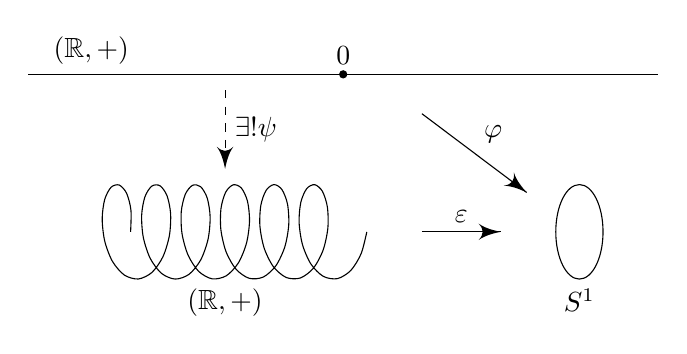
\begin{tikzpicture}
      \draw (-4, 0) -- (4, 0) node [pos=0.1, above] {$(\R, +)$};
      \node [circ] {};
      \node [above] {0};

      \draw [samples=80, domain=0:6] plot [smooth] ({-3 + 0.3 * cos (360 * \x) + \x / 2}, {-2 + 0.6 * sin (360 * \x)});
      \draw (3, -2) ellipse (0.3 and 0.6);

      \node [below] at (-1.5, -2.6) {$(\R, +)$};
      \node [below] at (3, -2.6) {$S^1$};

      \draw [->] (1, -2) -- +(1, 0) node [pos=0.5, above] {$\varepsilon$};
      \draw [->] (1, -0.5) -- (2.33, -1.5) node [pos=0.5, anchor = south west] {$\varphi$};
      \draw [->, dashed] (-1.5, -0.2) -- (-1.5, -1.2) node [pos=0.5, right] {$\exists ! \psi$};

    \end{tikzpicture}
  \end{center}
  The lifting is constructed by starting with $\psi(0) = 0$, and then extending a small interval at a time to get a continuous map $\R \to \R$. We will not go into the details. Alternatively, this follows from the lifting criterion from IID Algebraic Topology.

  We now claim that if in addition $\varphi$ is a homomorphism, then so is its continuous lifting $\psi$. If this is true, then we can conclude that $\psi(x) = cx$ for some $c\in \R$. Hence
  \[
    \varphi(x) = e^{icx}.
  \]
  To show that $\psi$ is indeed a homomorphism, we have to show that $\psi(x + y) = \psi(x) + \psi(y)$.

  By definition, we know
  \[
    \varphi(x + y) = \varphi(x) \varphi(y).
  \]
  By definition of $\psi$, this means
  \[
    \varepsilon(\psi(x + y) - \psi(x) - \psi(y)) = 1.
  \]
  We now look at our definition of $\varepsilon$ to get
  \[
    \psi(x + y) - \psi(x) - \psi(y) = 2 k \pi
  \]
  for some integer $k \in \Z$, depending \emph{continuously} on $x$ and $y$. But $k$ can only be an integer. So it must be constant. Now we pick our favorite $x$ and $y$, namely $x = y = 0$. Then we find $k = 0$. So we get
  \[
    \psi(x + y) = \psi(x) + \psi(y).
  \]
  So $\psi$ is a group homomorphism.
\end{proof}

With these two lemmas, we can prove our characterization of the (one-dimensional) representations of $S^1$.
\begin{thm}
  Every one-dimensional (continuous) representation $S^1$ is of the form
  \[
    \rho: z \mapsto z^n
  \]
  for some $n \in \Z$.
\end{thm}

\begin{proof}
  Let $\rho: S^1 \to \C^\times$ be a continuous representation. We now claim that $\rho$ actually maps $S^1$ to $S^1$. Since $C^1$ is compact, we know $\rho(S^1)$ has closed and bounded image. Also,
  \[
    \rho(z^n) = (\rho(z))^n
  \]
  for all $n \in \Z$. Thus for each $z \in S^1$, if $|\rho(z)| > 1$, then the image of $\rho(z^n)$ is unbounded. Similarly, if it is less than $1$, then $\rho(z^{-n})$ is unbounded. So we must have $\rho(S^1) \subseteq S^1$. So we get a continuous homomorphism
  \begin{align*}
    \R &\to S^1\\
    x &\mapsto \rho(e^{ix}).
  \end{align*}
  So we know there is some $c \in \R$ such that
  \[
    \rho(e^{ix}) = e^{icx},
  \]
  Now in particular,
  \[
    1 = \rho(e^{2 \pi i}) = e^{2\pi i c}.
  \]
  This forces $c \in \Z$. Putting $n = c$, we get
  \[
    \rho(z) = z^n.
  \]
\end{proof}
That has taken nearly an hour, and we've used two not-so-trivial facts from analysis. So we actually had to work quite hard to get this. But the result is good. We have a \emph{complete} list of representations, and we don't have to fiddle with things like characters.

Our next objective is to repeat this for $\SU(2)$, and this time we cannot just get away with doing some analysis. We have to do representation theory properly. So we study the general theory of representations of complex spaces.

In studying finite groups, we often took the ``average'' over the group via the operation $\frac{1}{|G|} \sum_{g \in G}\text{something}$. Of course, we can't do this now, since the group is infinite. As we all know, the continuous analogue of summing is called integration. Informally, we want to be able to write something like $\int_G \;\d g$.

This is actually a measure, called the ``Haar measure'', and always exists as long as you are compact and Hausdorff. However, we will not need or use this result, since we can construct it by hand for $S^1$ and $\SU(2)$.

\begin{defi}[Haar measure]
  Let $G$ be a topological group, and let
  \[
    \mathcal{C}(G) = \{f: G \to \C: f\text{ is continuous}, f(gxg^{-1})f(x)\text{ for all }g, x \in G\}.
  \]
  A non-trivial linear functional $\int_G: \mathcal{C}(G) \to C$, written as
  \[
    \int_G f = \int_G f(g) \;\d g
  \]
  is called a \emph{Haar measure} if
  \begin{enumerate}
    \item It satisfies the normalization condition
      \[
        \int_G 1 \;\d g = 1
      \]
      so that the ``total volume'' is $1$.
    \item It is left and right translation invariant, ie.
      \[
        \int_G f(xg)\;\d g = \int_G f(g)\;\d g = \int_G f(gx) \;\d g
      \]
      for all $x \in G$.
  \end{enumerate}
\end{defi}

\begin{eg}
  For a finite group $G$, we can define
  \[
    \int_G f(g)\;\d g = \frac{1}{|G|} \sum_{g \in G} f(g)\;\d g.
  \]
  The division by the group order is the thing we need to make the normalization hold.
\end{eg}

\begin{eg}
  Let $G = S^1$. Then we can have
  \[
    \int_G f(g)\;\d g = \frac{1}{2\pi} \int_0^{2\pi} f(e^{i\theta})\;\d \theta.
  \]
  Again, division by $2\pi$ is the normalization required.
\end{eg}

We have explicitly constructed them here, but there is a theorem that guarantees the existence of such a measure for sufficiently nice topological group.

\begin{thm}
  Let $G$ be a compact Hausdorff topological group. Then there exists a unique Haar measure on $G$.
\end{thm}
From now on, the word ``compact'' will mean ``compact and Hausdorff'', so that the conditions of the above theorem holds.

We will not prove theorem, and just assume it to be true. If you don't like this, whenever you see ``compact group'', replace it with ``compact group with Haar measure''. We will explicitly construct it for $\SU(2)$ later, which is all we really care about.

Once we know the existence of such a thing, most of the things we know for finite groups hold for compact groups, as long as we replace the sums with the appropriate integrals.

\begin{cor}[Weyl's unitary trick]
  Let $G$ be a compact group. Then every representation $(\rho, V)$ has a $G$-invariant Hermitian inner product.
\end{cor}

\begin{proof}
  As for the finite case, take any inner product $(\ph, \ph)$ on $V$, then define a new inner product by
  \[
    \bra \mathbf{v}, \mathbf{w}\ket = \int_G (\rho(g)\mathbf{v}, \rho(g)\mathbf{w})\;\d g.
  \]
  Then this is a $G$-invariant inner product.
\end{proof}

\begin{thm}[Maschke's theoerm]
  Let $G$ be compact group. Then every representation of $G$ is completely reducible.
\end{thm}

\begin{proof}
  Given a representation $(\rho, V)$. Choose a $G$-invariant inner product. If $V$ is not irreducible, let $W \leq V$ be a subrepresentation. Then $W^\perp$ is also $G$-invariant, and
  \[
    V = W \oplus W^\perp.
  \]
  Then the result follows by induction.
\end{proof}

We can use the Haar measure to endow $\mathcal{C}(G)$ with an inner product given by
\[
  \bra f, f'\ket = \int_G \overline{f(g)} f'(g) \;\d g.
\]
\begin{defi}[Character]
  If $\rho: G \to \GL(V)$ is a representation, then the \emph{character} $\chi_\rho = \tr \rho$ is a continuous class function, since each component $\rho(g)_{ij}$ is continuous.
\end{defi}

So characters make sense, and we can ask if all the things about finite groups hold here. For example, we can ask about orthogonality.

Schur's lemma also hold, with the same proof, since we didn't really need finiteness there. Using that, we can prove the following:

\begin{thm}[Orthogonality]
  Let $G$ be a compact group, and $V$ and $W$ be irreducible representations of $G$. Then
  \[
    \bra \chi_V, \chi_W\ket =
    \begin{cases}
      1 & V \cong W\\
      0 & V \not\cong W
    \end{cases}.
  \]
\end{thm}

Now do irreducible characters form a basis for $\mathcal{C}(G)$?
\begin{eg}
  We take the only (infinite) compact group we know about --- $G = S^1$. We have found that the one-dimensional representations are
  \[
    \rho_n: z \mapsto z^n
  \]
  for $n \in \Z$. As $S^1$ is abelian, these are all the (continuous) irreducible representations --- given \emph{any} representation $\rho$, we can find a simultaneous eigenvector for each $\rho(g)$.

  The ``character table of $S^1$'' has rows $\chi_n$ indexed by $\Z$, with $\chi_n(e^{i\theta}) = e^{in\theta}$.

  Now given any representation of $S^1$, say $V$, we can break $V$ as a direct sum of $1$-dimensional subrepresentations. So the character $\chi_V$ of $V$ is of the form
  \[
    \chi_V(z) = \sum_{n \in \Z} a_n z^n,
  \]
  where $a_n \in \Z_{\geq 0}$, and only finitely many $a_n$ are non-zero (since we are assuming finite-dimensionality).

  Actually, $a_n$ is the number of copies of $\rho_n$ in the decomposition of $V$. We can find out the value of $a_n$ by computing
  \[
    a_n = \bra \chi_n, \chi_V\ket = \frac{1}{2\pi} \int_0^{2\pi} e^{-in\theta}\chi_V(e^{i\theta})\;\d \theta.
  \]
  Hence we know
  \[
    \chi_V(e^{i\theta}) = \sum_{n \in \Z} \left(\frac{1}{2\pi} \int_0^{2\pi} \chi_V(e^{i\theta'}) e^{-in\theta'}\;\d \theta'\right) e^{in\theta}.
  \]
  This is really just a Fourier decomposition of $\chi_V$. This gives a decomposition of $\chi_V$ into irreducible characters, and the ``Fourier mode'' $a_n$ is the number of each irreducible character occurring in this decomposition.

  It is possible to show that $\chi_n$ form a complete orthonormal set in the Hilbert space $L^2(S^1)$, ie. square-integrable functions on $S^1$. This is the Peter-Weyl theorem, and is highly non-trivial.
\end{eg}

In the rest of the time, we would like to talk about $G = \SU(2)$.

Recall that
\[
  \SU(2) = \{A \in \GL_2(\C): A^\dagger A = I, \det A = I\}.
\]
Note that if
\[
  A =
  \begin{pmatrix}
    a & b\\
    c & d
  \end{pmatrix} \in \SU(2),
\]
then since $\det A = 1$, we have
\[
  A^{-1} =
  \begin{pmatrix}
    d & -b\\
    -c & a
  \end{pmatrix}.
\]
So we need $d = \bar{a}$ and $c = -\bar{b}$. Moreover, we have
\[
  a\bar{a} + b\bar{b} = 1.
\]
Hence we can write $\SU(2)$ explicitly as
\[
  G = \left\{
    \begin{pmatrix}
      a & b\\
      -\bar{b} & \bar{a}
    \end{pmatrix}: a, b \in \C, |a|^2 + |b|^2 = 1
  \right\}.
\]
Topologically, we know $G \cong S^3 \subseteq \C^2 \cong \R^4$.

Instead of thinking about $\C^2$ in the usual vector space way, we can think of it as a subgroup of $M_2(\C)$ via
\[
  \H = \left\{
    \begin{pmatrix}
      z & w\\
      -\bar{w} & \bar{z}
    \end{pmatrix}:
  w, z \in \C\right\} \leq M_2(\C).
\]
This is known as \emph{Hamilton's quaternion algebra}. Then $\H$ is a 4-dimensional Euclidean space (two components from $z$ and two components from $w$), with a norm on $H$ given by
\[
  \|A\|^2 = \det A.
\]
We now see that $\SU(2) \leq \H$ is exactly the unit sphere $\|A\|^2 = 1$ in $\H$. If $A \in \SU(2)$ and $x \in \H$, then $\|Ax\| = \|x\|$ since $\|A\| = 1$. So elements of $G$ acts as isometries on the space. Hence after normalization (by $\frac{1}{2\pi^2}$), the usual integration of functions on $S^3$ defines a Haar measure on $G$. It is an exercise on the last example sheet to write this out explicitly.

We now look at conjugacy in $G$. We let
\[
  T = \left\{
    \begin{pmatrix}
      a & 0\\
      0 & \bar{a}
    \end{pmatrix}: a \in \C, |a|^2 = 1
  \right\} \cong S^1.
\]
This is the \emph{maximal torus} in $G$, and it plays a fundamental role, since we happen to know about $S^1$. We also have a favorite element
\[
  s =
  \begin{pmatrix}
    0 & 1\\
    -1 & 0
  \end{pmatrix} \in \SU(2).
\]
We now prove some easy linear algebra results about $\SU(2)$.
\begin{lemma}[$\SU(2)$-conjugacyy classes]\leavevmode
  \begin{enumerate}
    \item Let $t \in T$. Then $sts^{-1} = t^{-1}$.
    \item $s^2 = -I \in \Z(\SU(2))$.
    \item The normalizer
      \[
        N_G(T) = T \cup sT =
        \left\{
          \begin{pmatrix}
            a & 0\\
            0 & \bar{a}
          \end{pmatrix},
          \begin{pmatrix}
            0 & a\\
            -\bar{a} & 0
          \end{pmatrix}: a\ in \C, |a| = 1\right\}.
      \]
    \item Every conjugacy class $\mathcal{C}$ of $\SU(2)$ contains an element of $T$, ie. $\mathcal{C} \cap T \not= \emptyset$.

    \item In fact,
      \[
        \mathcal{C} \cap T = \{t, t^{-1}\}
      \]
      for some $t \in T$, and $t = t^{-1}$ if and only if $t = \pm I$, in which case $\mathcal{C} = \{t\}$.
    \item There is a bijection
      \[
        \{\text{conjugacy classes in }\SU(2)\} \leftrightarrow [-1, 1],
      \]
      given by
      \[
        A \mapsto \frac{1}{2} \tr A.
      \]
      We can see that if
      \[
        A =
        \begin{pmatrix}
          \lambda & 0\\
          0 & \bar{\lambda}
        \end{pmatrix},
      \]
      then
      \[
        \frac{1}{2}\tr A = \frac{1}{2}(\lambda + \bar{\lambda}) = \Re(\lambda).
      \]
  \end{enumerate}
\end{lemma}
Note that what (iv) and (v) really say is that matrices in $\SU(2)$ are diagonalizable (over $\SU(2)$).

\begin{proof}\leavevmode
  \begin{enumerate}
    \item Write it out.
    \item Write it out.
    \item Direct verification.
    \item It is well-known from linear algebra that every unitary matrix $X$ has an orthonormal basis of eigenvectors, and hence is conjugate in $U(2)$ to one in $T$, say
      \[
        Q X Q^\dagger \in T.
      \]
      We now want to force $Q$ into $\SU(2)$, ie. make $Q$ have determinant $1$.

      We put $\delta = \det Q$. Since $Q$ is unitary, ie. $QQ^\dagger = I$, we know $|\delta| = 1$. So we let $\varepsilon$ be a square root of $\delta$, and define
      \[
        Q_1 = \varepsilon^{-1} Q.
      \]
      Then we have
      \[
        Q_1 X Q_1^{\dagger} \in T.
      \]
    \item We let $g \in G$, and suppose $g \in \mathcal{C}$. If $g = \pm I$, then $\mathcal{C} \cap T = \{g\}$. Otherwise, $g$ has two distinct eigenvalues $\lambda, \lambda^{-1}$. Note that the two eigenvlaues must be inverses of each other, since it is in $\SU(2)$. Then we know
      \[
        \mathcal{C} = \left\{h
          \begin{pmatrix}
            \lambda & 0\\
            0 & \lambda^{-1}
          \end{pmatrix}h^{-1} : h \in G
        \right\}.
      \]
      Thus we find
      \[
        \mathcal{C} \cap T = \left\{
          \begin{pmatrix}
            \lambda & 0\\
            0 & \lambda^{-1}
          \end{pmatrix},
          \begin{pmatrix}
            \lambda^{-1} & 0\\
            0 & \lambda
          \end{pmatrix}
        \right\}.
      \]
      This is true since eigenvalues are preserved by conjugation, so if any
      \[
        \begin{pmatrix}
          \mu & 0\\
          0 & \mu^{-1}
        \end{pmatrix},
      \]
      then $\{\mu, \mu^{-1}\} = \{\lambda, \lambda^{-1}\}$. Also, we can get the second matrix from the first by conjugating with $s$.
    \item Consider the map
      \[
        \frac{1}{2} \tr: \{\text{conjugacy classes}\} \to [-1, 1].
      \]
      By (v), matrices are conjugate in $G$ iff they have the same set of eigenvalues. Now
      \[
        \frac{1}{2}\tr
        \begin{pmatrix}
          \lambda & 0\\
          0 & \lambda^{-1}
        \end{pmatrix}
        = \frac{1}{2}(\lambda + \bar{\lambda}) = \Re(\lambda) = \cos \theta,
      \]
      where $\lambda = e^{i\theta}$. Hence the map is a surjection onto $[-1, 1]$.

      Now we have to show it is injective. This is also easy. If $g$ and $g'$ have the same image, ie.
      \[
        \frac{1}{2} \tr g = \frac{1}{2} \tr g',
      \]
      then $g$ and $g'$ have the same characteristic polynomial, namely
      \[
        x^2 - (\tr g)x + 1.
      \]
      Hence they have the same eigenvalues, and hence they are similar.
  \end{enumerate}
\end{proof}

We now write, for $t \in (-1, 1)$,
\[
  \mathcal{C}_t = \left\{g \in G: \frac{1}{2} \tr g = t\right\}.
\]
In particular, we have
\[
  \mathcal{C}_1 = \{I\}, \quad \mathcal{C}_{-1} = \{-I\}.
\]
\begin{prop}
  For $t \in (-1, 1)$, the class $\mathcal{C}_t \cong S^2$ as topological spaces.
\end{prop}
This is not really needed, but is a nice thing to know.
\begin{proof}
  Exercise! % exercise for the reader
\end{proof}

\subsection{Representations of \texorpdfstring{$\SU(2)$}{SU(2)}}
We now move on to classify the irreducible representations of $\SU(2)$.

We let $V_n$ be the complex space of all homogeneous polynomials of degree $n$ in variables $x, y$, ie.
\[
  V_n = \{r_0 x^n + r_1 x^{n - 1}y + \cdots + r_n y^n: r_0, \cdots, r_n \in \C\}.
\]
This is an $n + 1$-dimensional complex vector space with basis $x^n, x^{n - 1}y, \cdots, y^n$.

We want to get an action of $\SU(2)$ on $V_n$. It is easier to think about the action of $\GL_2(\C)$ in general, and then restrict to $\SU(2)$. We define the action of $\GL_2(\C)$ on $V_n$ by
\[
  \rho_n: \GL_2(\C) \to \GL(v)
\]
given by the rule
\[
  \rho_n\left(
  \begin{pmatrix}
    a & b\\
    c & d
  \end{pmatrix}\right) f(x, y) = f(ax + cy, bx + dy).
\]
In other words, we have
\[
  \rho_n\left(
  \begin{pmatrix}
    a & b\\
    c & d
  \end{pmatrix}\right) f\left(
  \begin{pmatrix}
    x & y
  \end{pmatrix}\right) = f\left(
  \begin{pmatrix}
    x & y
  \end{pmatrix}
  \begin{pmatrix}
    a & b\\
    c & d
  \end{pmatrix}\right),
\]
where the multiplication in $f$ is matrix multiplication.

\begin{eg}
  When $n = 0$, then $V_0 \cong \C$, and $\rho_0$ is the trivial representation.

  When $n = 1 $, then this is the natural two-dimensional representation, and
  \[
    \rho_1\left(
    \begin{pmatrix}
      a & b\\
      c & d
    \end{pmatrix}
    \right)
  \]
  has matrix
  \[
    \begin{pmatrix}
      a & b\\
      c & d
    \end{pmatrix}
  \]
  with respect to the standard basis $\{x, y\}$ of $V_1 = \C^2$.

  More interestingly, when $n = 2$, we know
  \[
    \rho_2\left(
    \begin{pmatrix}
      a & b\\
      c & d
    \end{pmatrix}
    \right)
  \]
  has matrix
  \[
    \begin{pmatrix}
      a^2 & ab & b^2\\
      2ac & ad + bc & 2bd\\
      c^2 & cd & d^2
    \end{pmatrix},
  \]
  with respect to the basis $x^2, xy, y^2$ of $V_2 = \C^3$. We obtain the matrix by computing, eg.
  \[
    \rho_2(g) (x^2) = (ax + cy)^2 = a^x x^2 + 2ac xy + c^2 y^2.
  \]
\end{eg}

Now we know $\SU(2) \leq \GL_2(\C)$. So we can view $V_n$ as a representation of $\SU(2)$ by restriction.

Now we've got some representations. The claim is that these are all the irreducibles. Before we prove that, we look at the character of these things.

\begin{lemma}
  A continuous class function $f: G \to \C$ is determined by its restriction to $T$, and $F|_T$ is even, ie.
  \[
    f\left(
    \begin{pmatrix}
      \lambda & 0\\
      0 & \lambda^{-1}
    \end{pmatrix}
    \right) =
    f\left(
    \begin{pmatrix}
      \lambda^{-1} & 0\\
      0 & \lambda
    \end{pmatrix}
    \right).
  \]
\end{lemma}

\begin{proof}
  Each conjugacy class in $\SU(2)$ meets $T$. So a class function is determined by its restriction to $T$. Evenness follows from the fact that the two elements are conjugate.
\end{proof}

In particular, a character of a representation $(\rho, V)$ is also an even function $\chi_\rho: S^1 \to \C$.

\begin{lemma}
  If $\chi$ is a character of a representation of $\SU(2)$, then its restriction $\chi|_T$ is a Laurent polynomial, ie. a finite $\N$-linear combination of functions
  \[
    \begin{pmatrix}
      \lambda & 0\\
      0 & \lambda^{-1}
    \end{pmatrix} \mapsto \lambda^n
  \]
  for $n \in \Z$.
\end{lemma}

\begin{proof}
  If $V$ is a representation of $\SU(2)$, then $\Res_T^{\SU(2)} V$ is a representation of $T$, and its character $\Res_T^{\SU(2)} \chi$ is the restriction of $\chi_V$ to $T$. But every representation of $T$ has its character of the given form. So done.
\end{proof}

\begin{notation}
  We write $\N[z, z^{-1}]$ for the set of all Laurent polynomials, ie.
  \[
    \N[z, z^{-1}] = \left\{\sum a_n z^n: a_n \in \N: \text{only finitely many $a_n$ non-zero}\right\}.
  \]
  We further write
  \[
    \N[z, z^{-1}]_{\mathrm{ev}} = \{f \in \N[z, z^{-1}]: f(z) = f(z^{-1})\}.
  \]
\end{notation}
Then by our lemma, for every continuous representation $V$ of $\SU(2)$, the character $\chi_V \in \N[z, z^{-1}]_{\mathrm{ev}}$ (by identifying it with its restriction to $T$).

We now actually calculate the character $\chi_n$ of $(\rho_n, V_n)$ as a representation of $\SU(2)$. We have
\[
  \chi_{V_n}(g) = \tr \rho_n (g),
\]
where
\[
  g \sim
  \begin{pmatrix}
    z & 0\\
    0 & z^{-1}
  \end{pmatrix} \in T.
\]
Then we have
\[
  \rho_n \left(
  \begin{pmatrix}
    z & 0\\
    0 & z^{-1}
  \end{pmatrix}\right)(x^i y^j) = (zx^i)(z^{-1}y^j) = z^{i - j} x^i y^j.
\]
So each $x^i y^j$ is an eigenvector of $\rho_n (g)$, with eigenvalue $z^{i - j}$. So we know $\rho_n (g)$ has a matrix
\[
  \begin{pmatrix}
    z^n\\
    & z^{n - 2}\\
    & & \ddots\\
    & & & z^{2 - n}\\
    & & & & z^{-n}
  \end{pmatrix},
\]
with respect to the standard basis. Hence the character is just
\[
  \chi_n\left(
  \begin{pmatrix}
    z & 0\\
    0 & z^{-1}
  \end{pmatrix}\right) = z^n + z^{n - 2} + \cdots + z^{-n} = \frac{z^{n + 1} - z^{-(n + 1)}}{z - z^{-1}},
\]
where the last expression is valid unless $z = \pm 1$.

We can now state the result we are aiming for:
\begin{thm}
  The representations $\rho: \SU(2) \to \GL(V_n)$ of dimension $n + 1$ are irreducible for $n \in \Z_{\geq 0}$.
\end{thm}
Again, we get a complete set. A complete list of all irreducible representations (proven later), given in a really nice form. This is spectacular.

\begin{proof}
  Let $0 \not= W \leq V_n$ be a $G$-invariant subspace, ie. a subrepresentation of $V_n$. We will show that $W = V_n$.

  All we know about $W$ is that it is non-zero. So we take some non-zero vector of $W$.
  \begin{claim}
    Let
    \[
      0 \not= w = \sum_{j = 0}^n r_j x^{n - j}y^j \in W.
    \]
    Since this is non-zero, there is some $i$ such that $r_i \not= 0$. The claim is that $x^{n - i}y^i \in W$.
  \end{claim}
  We argue by induction on the number of non-zero coefficients $r_j$. If there is only one non-zero coefficient, then we are already done, as $w$ is a non-zero scalar multiple of $x^{n - i}y^i$.

  So assume there is more than one, and choose one $i$ such that $r_i \not= 0$. We pick $z \in S^1$ with $z^n, z^{n - 2}, \cdots, z^{2 - n}, z^{-n}$ all distinct in $\C$. Now
  \[
    \rho_n\left(
    \begin{pmatrix}
      z\\&z^{-1}
    \end{pmatrix}\right)w = \sum r_j z^{n - 2j} x^{n - j}y^j \in W.
  \]
  Subtracting a copy of $w$, we find
  \[
    \rho_n\left(
    \begin{pmatrix}
      z\\&z^{-1}
    \end{pmatrix}\right)w - z^{n - 2i}w = \sum r_j (z^{n - 2j} - z^{n - 2i})x^{n - j}y^j \in W.
  \]
  We now look at the coefficient
  \[
    r_j (z^{n - 2j} - z^{n - 2i}).
  \]
  This is non-zero if and only if $r_j$ is non-zero and $j \not= i$.

  Thus the number of non-zero coefficients is exactly one less than our $w$. So by induction, we know
  \[
    x^{n - j}y^j \in W
  \]
  for all $j \not= i$ and $r_j \not= 0$. thus we know
  \[
    x^{n -i}y^i = \frac{1}{r_i} \left(w - \sum_{j \not= i} r_j x^{n - j}y^j\right) \in W,
  \]
  as claimed.

  This gives us one basis vector inside $W$, and we need to get the rest.

  \begin{claim}
    $W = V_n$.
  \end{claim}
  We now know that $x^{n - i}y^i \in W$ for some $i$. We consider
  \[
    \rho_n\left(\frac{1}{\sqrt{2}}
    \begin{pmatrix}
      1 & -1\\
      1 & 1
    \end{pmatrix}\right) x^{n - i}y^i = \frac{1}{\sqrt{2}} (x + y)^{n - i}(-x + y)^i \in W.
  \]
  It is clear that the coefficient of $x^n$ is non-zero. So we can use the claim to deduce $x^n \in W$.

  Finally, for general $a, b \not= 0$, we apply
  \[
    \rho_n\left(
    \begin{pmatrix}
      a & -\bar{b}\\
      b &\bar{a}
    \end{pmatrix}\right) x^n = (ax + by)^n \in W,
  \]
  and the coefficient of everything is non-zero. So basis vectors are in $W$. So $W = V_n$.
\end{proof}
This proof is surprisingly elementary. It does not use any technology at all.

Alternatively, to prove this, we can identify
\[
  \mathcal{C}_{\cos \theta} \left\{A \in G: \frac{1}{2}\tr A = \cos \theta \right\}
\]
with the $2$-sphere
\[
  \{ |\Im a|^2 + |b|^2 = \sin^2 \theta\}
\]
of radius $\sin \theta$. So if $f$ is a class function on $G$, since $f$ is constant on each class $\mathcal{C}_{\cos \theta}$, we know
\[
  \int_G f(g)\;\d g = \frac{1}{2\pi^2}\int_0^{2\pi} \frac{1}{2}f\left(
  \begin{pmatrix}
    e^{i\theta}\\
    &e^{-i\theta}
  \end{pmatrix}\right) 4\pi \sin^2 \theta\;\d \theta.
\]
This is the \emph{Weyl integration formula}, which is the Haar measure for $\SU(2)$. Then if $\chi_n$ is the character of $V_n$, we can show that $\bra \chi_n, \chi_n\ket = 1$. Hence $\chi_n$ is irreducible. We will not go into the details of this construction.

\begin{thm}
  Every finite-dimensional continuous irreducible representation of $G$ is one of the $\rho_n: G \to \GL(V_n)$ as defined above.
\end{thm}

\begin{proof}
  Assume $\rho_V: G \to \GL(V)$ is an irreducible representation affording a character $\chi_V \in \N[z, z^{-1}]_{\mathrm{ev}}$. We will show that $\chi_V = \chi_n$ for some $n$. Now we see
  \begin{align*}
    \chi_0 &= 1\\
    \chi_1 &= z + z^{-1}\\
    \chi_2 &= z^2 +1 + z^{-2}\\
    &\;\;\vdots
  \end{align*}
  form a basis of $\Q[z, z^{-1}]_{\mathrm{ev}}$, which is a non-finite dimensional vector space over $\Q$. Hence we can write
  \[
    \chi_V = \sum_n a_n \chi_n,
  \]
  a finite sum with finitely many $a_n\not= 0$. Note that it is possible that $a_n \in \Q$. So we clear denominators, and move the summands with negative coefficients to the left hand side. So we get
  \[
    m \chi_V + \sum_{i \in I} m_i \chi_i = \sum_{j \in J} n_j \chi_j,
  \]
  with $I, J$ disjoint finite subsets of $\N$, and $m, m_i, n_j \in \N$.

  We know the left and right-hand side are characters of representations of $G$. So we get
  \[
    m V \oplus \bigoplus_I m_i V_i = \bigoplus_J n_j V_j.
  \]
  Since $V$ is irreducible and factorization is unique, we must have $V \cong V_n$ for some $n \in J$.
\end{proof}

We've got a complete list of irreducible representations of $\SU(2)$. So we can look at what happens when we take products.

We know that for $V, W$ representations of $\SU(2)$, if
\[
  \Res_T^{\SU(2)}V \cong \Res_T^{\SU(2)}W,
\]
then in fact
\[
  V \cong W.
\]
This gives us the following result:
\begin{prop}
  Let $G = \SU(2)$ or $G = S^1$, and $V, W$ are representations of $G$. Then
  \[
    \chi_{V \otimes W} = \chi_V \chi_W.
  \]
\end{prop}

\begin{proof}
  By the previous remark, it is enough to consider the case $G = S^1$. Suppose $V$ and $W$ have eigenbases $\mathbf{e}_1, \cdots, \mathbf{e}_n$ and $\mathbf{f}_1, \cdots, \mathbf{f}_m$ respectively such that
  \[
    z \mathbf{e}_i = z^{n_i} \mathbf{e}_i,\quad z \mathbf{f}_j = z^{m_j} \mathbf{f}_j
  \]
  for each $i, j$ (note that multiplication on the left is the group action, and multiplication on the right is scalar multiplication). Then
  \[
    z(\mathbf{e}_i\otimes \mathbf{f}_j) = z^{n_i + m_j} \mathbf{e}_i \otimes \mathbf{f}_j.
  \]
  Thus the character is
  \[
    \chi_{V \otimes W}(z) = \sum_{i, j} z^{n_i + m_j} = \left(\sum_i z^{n_i}\right) \left(\sum_j z^{m_j}\right) = \chi_V(z) \chi_W(z).
  \]
\end{proof}

\begin{eg}
  We have
  \[
    \chi_{V_1 \otimes V_1}(z) = (z + z^{-1})^2 = z^2 + 2 + z^{-2} = \chi_{V_2} + \chi_{V_0}.
  \]
  So we have
  \[
    V_1 \otimes V_1 \cong V_2 \oplus V_0.
  \]
  Similarly, we can compute
  \[
    \chi_{V_1 \otimes V_2}(z) = (z^2 + 1 + z^{-2})(z + z^{-1}) = z^3 + 2z + 2z^{-1} + z^{-3} = \chi_{V_3} + \chi_{V_1}.
  \]
  So we get
  \[
    V_1 \otimes V_2 \cong V_3 \oplus V_1.
  \]
\end{eg}

\begin{prop}[Clebsch-Gordon rule]
  For $n, m \in \N$, we have
  \[
    V_n \otimes V_m \cong V_{n + m} \oplus V_{n + m - 2} \oplus \cdots \oplus V_{|n - m| + 2} \oplus V_{|n - m|}.
  \]
\end{prop}

\begin{proof}
  We just check this works for characters. Without loss of generality, we assume $n \geq m$. We can compute
  \begin{align*}
    (\chi_n \chi_m)(z) &= \frac{z^{n + 1} - z^{-n - 1}}{z - z^{-1}} (z^m + z^{m - 2} + \cdots + z^{-m})\\
    &= \sum_{j = 0}^m \frac{z^{n + m + 1 - 2j} - z^{2j - n - m - 1}}{z - z^{-1}}\\
    &= \sum_{j = 0}^m \chi_{n + m - 2j}(z).
  \end{align*}
  Note that the condition $n \geq m$ ensures there are no cancellations in the sum.
\end{proof}

\subsection{Representations of \texorpdfstring{$\SO(3)$}{SO(3)}}
We've now got a complete list of representations of $S^1$ and $\SU(2)$. We see if we can make some deductions about some related groups.

To begin with, we relate some other groups to the groups we already know about.
\begin{prop}
  There are isomorphisms of topological groups:
  \begin{enumerate}
    \item $\SO(3) \cong \SU(2)/ \{\pm I\} = \PSU(2)$
    \item $\SO(4) \cong \SU(2) \times \SU(2)/\{\pm (I, I)\}$
    \item $\U(2) \cong \U(1) \times \SU(2) / \{\pm (I, I)\}$
  \end{enumerate}
  All maps are group isomorphisms, but in fact also homeomorphisms. To show this, we can use the fact that a continuous bijection from a Hausdorff space to a compact space is automatically a homeomorphism.
\end{prop}
Assuming this is true, we obtain the following corollary;

\begin{cor}
  Every irreducible representation of $\SO(3)$ has the following form:
  \[
    \rho_{2m}: \SO(3) \to \GL(V_{2m}),
  \]
  for some $m \geq 0$.
\end{cor}

\begin{proof}
  Irreducible representations of $\SO(3)$ correspond to irreducible representations of $\SU(2)$ such that $-I$ acts trivially. But $-I$ acts on $V_n$ as $-1$ when $n$ is odd, and as $1$ when $n$ is even, since % why
  \[
    \rho(-I) =
    \begin{pmatrix}
      (-1)^n\\
      & (-1)^{n - 2}\\
      & & \ddots\\
      & & & (-1)^{-n}
    \end{pmatrix} = (-1)^n I.
  \]
\end{proof}

Finally, we provide a (sketch) proof of the isomorphism $\SO(3) \cong \SU(2) / \{\pm I\}$.

\begin{prop}
  $\SO(3) \cong \SU(2)/\{\pm I\}$.
\end{prop}

\begin{proof}[Proof sketch]
  Recall that $\SU(2)$ can be viewed as the sphere of unit norm quaternions $\H \cong \R^4$.

  Let
  \[
    \H^0 = \{A \in \H: \tr A = 0\}.
  \]
  These are the ``pure'' quaternions. This is a three-dimensional subspace of $\H$. It is not hard to see this is
  \[
    \H^0 = \R\left\bra
    \begin{pmatrix}
      i & 0\\
      0 & -i
    \end{pmatrix},
    \begin{pmatrix}
      0 & 1\\
      -1 & 0
    \end{pmatrix},
    \begin{pmatrix}
      0 & i\\
      i & 0
    \end{pmatrix}\right\ket = \R\left\bra \mathbf{i}, \mathbf{j}, \mathbf{k}\right\ket,
  \]
  where $\R\bra \cdots\ket$ is the $\R$-span of the things.

  This is equipped with the norm
  \[
    \|A\|^2 = \det A.
  \]
  This gives a nice $3$-dimensional Euclidean space, and $\SU(2)$ acts as isometries on $\H_0$ by conjugation, ie.
  \[
    X\cdot A = XAX^{-1},
  \]
  giving a group homomorphism
  \[
    \varphi: \SU(2) \to \Or(3),
  \]
  and the kernel of this map is $Z(\SU(2)) = \{\pm I\}$. We also know that $\SU(2)$ is compact, and $\Or(3)$ is Hausdorff. Hence the continuous group isomorphism
  \[
    \bar{\varphi}: \SU(2)/\{\pm I\} \to \im \varphi
  \]
  is a homeomorphism. It remains to show that $\im \varphi = \SO(3)$.

  But we know $\SU(2)$ is connected, and $\det (\varphi(X))$ is a continuous function that can only take values $1$ or $-1$. So $\det (\varphi(X))$ is either always $1$ or always $-1$. But $\det (\varphi(I)) = 1$. So we know $\det(\varphi(X)) = 1$ for all $X$. Hence $\im \varphi \leq \SO(3)$.

  To show that equality indeed holds, we have to show that all possible rotations in $\H^0$ are possible. We first show all rotations in the $\mathbf{i},\mathbf{j}$-plane are implemented by elements of the form $a + b\mathbf{k}$, and similarly for any permutation of $\mathbf{i}, \mathbf{j}, \mathbf{k}$. Since all such rotations generate $\SO(3)$, we are then done. Now consider
  \[
    \begin{pmatrix}
      e^{i\theta} & 0\\
      0 & e^{-i\theta}
    \end{pmatrix}
    \begin{pmatrix}
      ai & b\\
      -\bar{b} & -ai
    \end{pmatrix}
    \begin{pmatrix}
      e^{i\theta} & 0\\
      0 & e^{i\theta}
    \end{pmatrix}
    =
    \begin{pmatrix}
      ai & e^{2i\theta}b\\
      -\bar{b} e^{-2i\theta} & -ai
    \end{pmatrix}.
  \]
  So
  \[
    \begin{pmatrix}
      e^{i\theta} & 0\\
      0 & e^{-i\theta}
    \end{pmatrix}
  \]
  acts on $\R\bra \mathbf{i}, \mathbf{j}, \mathbf{k}\ket$ by a rotation in the $(\mathbf{j}, \mathbf{k})$-plane through an angle $2\theta$. We can check that
  \[
    \begin{pmatrix}
      \cos \theta & \sin \theta\\
      -\sin \theta & \cos \theta
    \end{pmatrix},\quad
    \begin{pmatrix}
      \cos \theta & i \sin \theta\\
      i\sin \theta & \cos \theta
    \end{pmatrix}
  \]
  act by rotation of $2\theta$ in the $(\mathbf{i}, \mathbf{k})$-plane and $(\mathbf{i}, \mathbf{j})$-plane respectively. So done.
\end{proof}

We can adapt this proof to prove the other isomorphisms. However, it is slightly more difficult to get the irreducible representations, since it involves taking some direct products. We need a result about products $G \times H$ of two compact groups. Similar to the finite case, we get the complete list of irreducible representations by taking the tensor products $V \otimes W$, where $V$ and $W$ range over the irreducibles of $G$ and $H$ independently.

\begin{prop}
  The complete list of irreducible representations of $\SO(4)$ is $\rho_m \times \rho_n$, where $m, n > 0$ and $m \equiv n \pmod 2$.
\end{prop}

\begin{prop}
  The complete list of irreducible representations of $\U(2)$ is
  \[
    \det{ }^{\otimes m} \otimes \rho_n,
  \]
  where $m, n \in \Z$ and $n \geq 0$.
\end{prop}
\end{document}
